% --------------------------------------------------------------------
% Anexos -------------------------------------------------------------

% Código para agregar el informe académico en formato PDF ------------
% 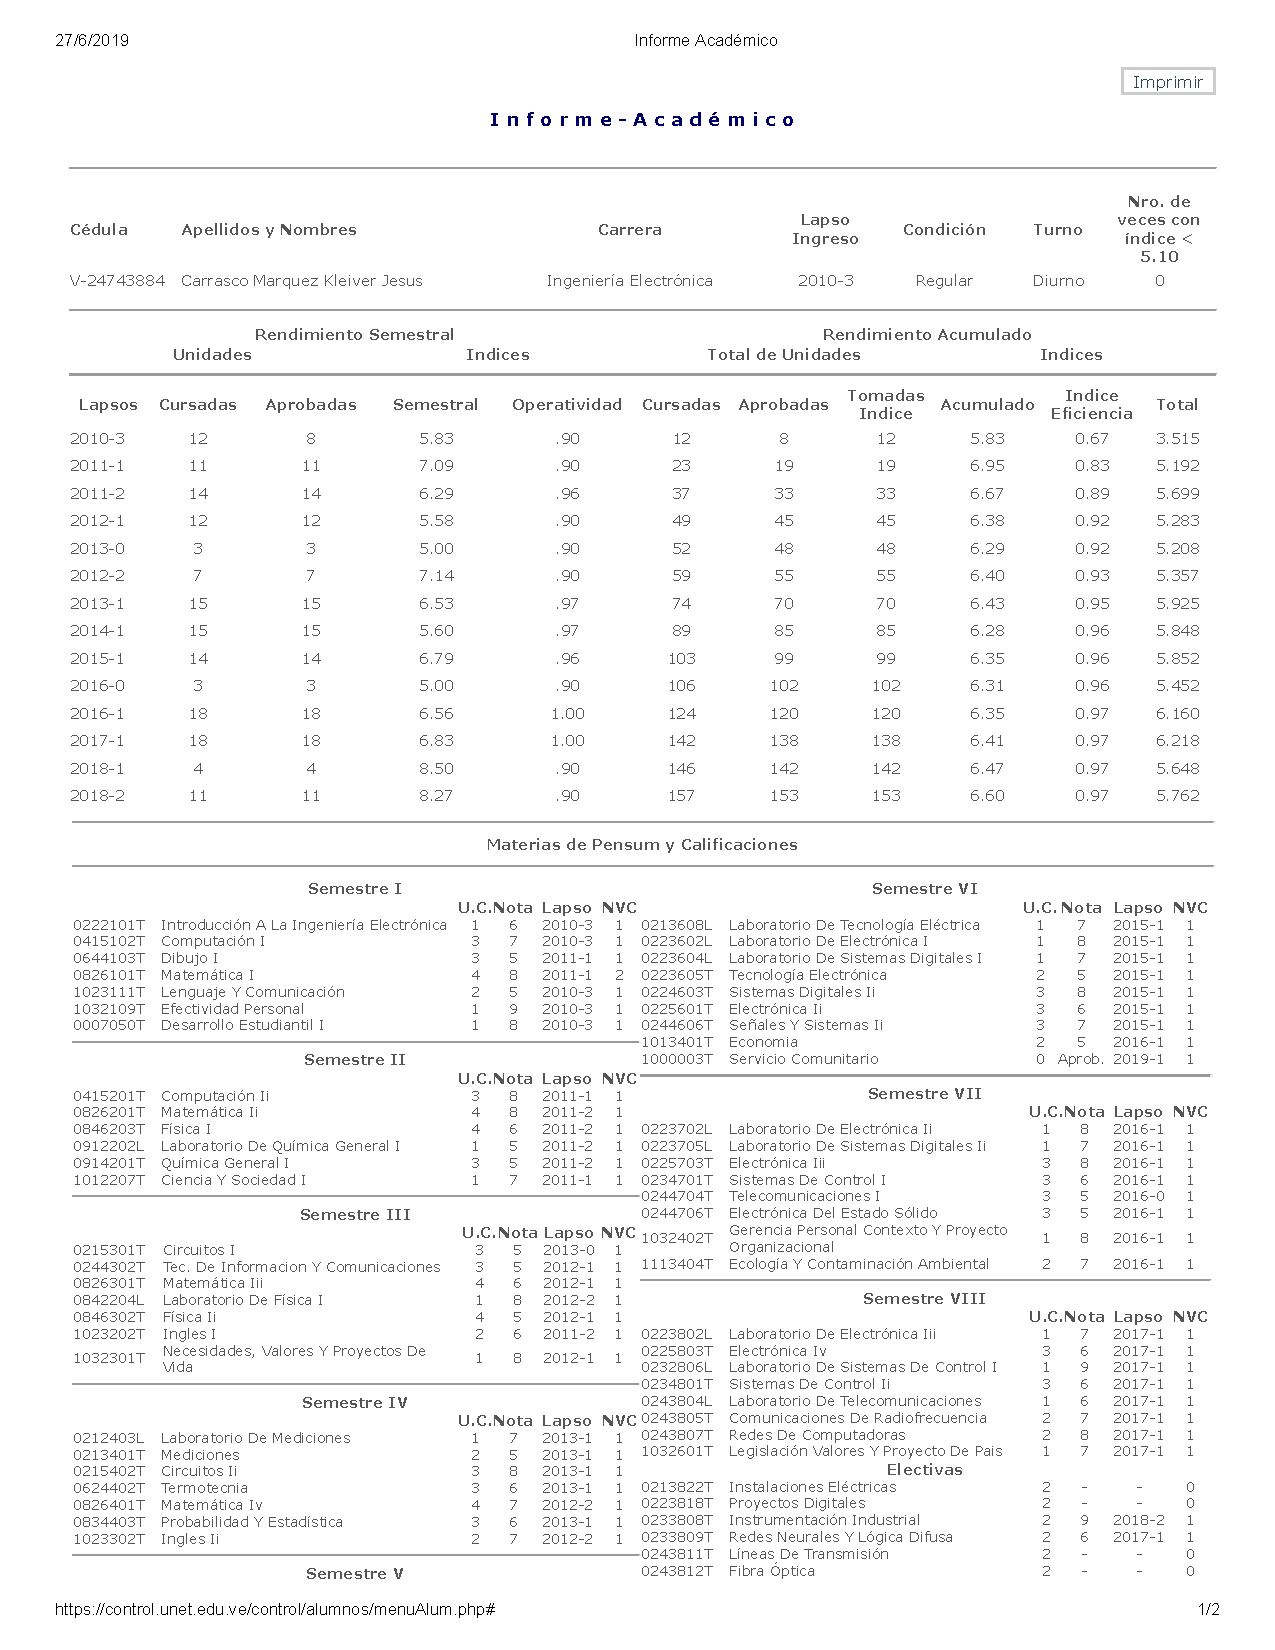
\includepdf[scale=0.7,pages=1,pagecommand={\AgregarAnexo{Informe académico}}, 
% addtotoc={1, chapter, 0,\bfseries\uppercase{Anexos}, pdf:informe}]{imagenes/informeAcademico}
% \includepdf[scale=0.7,pages=2, pagecommand={}]{imagenes/informeAcademico}
% --------------------------------------------------------------------
% Nota: Si se utiliza este código se deben comentar:
% \newpage
% \phantomsection
% \addcontentsline{toc}{chapter}{Anexos}
% --------------------------------------------------------------------
% Sintaxis para agregar un anexo:
%   \AgregarAnexo{Titulo del anexo}{anexo:label_del_anexo}
%   El anexo puede ser referenciado luego en el texto utilizando \ref{anexo:label_del_anexo}, si es el primer
%   anexo, se representara como [Anexo A] al utilizar \ref{}.

\newpage                                % Comentar si se incluye
\phantomsection                         % primero un pdf
\addcontentsline{toc}{chapter}{Anexos}  % Para evitar problemas TOC

% Para agregar anexos a la tesis
\AgregarAnexo{Interfaz gráfica de la función de análisis de sistemas de control}{anexo:interfazAnalisis}
    \begin{figure}[htb]
        \centering
        \begin{subfigure}[t]{\textwidth}
            \centering
            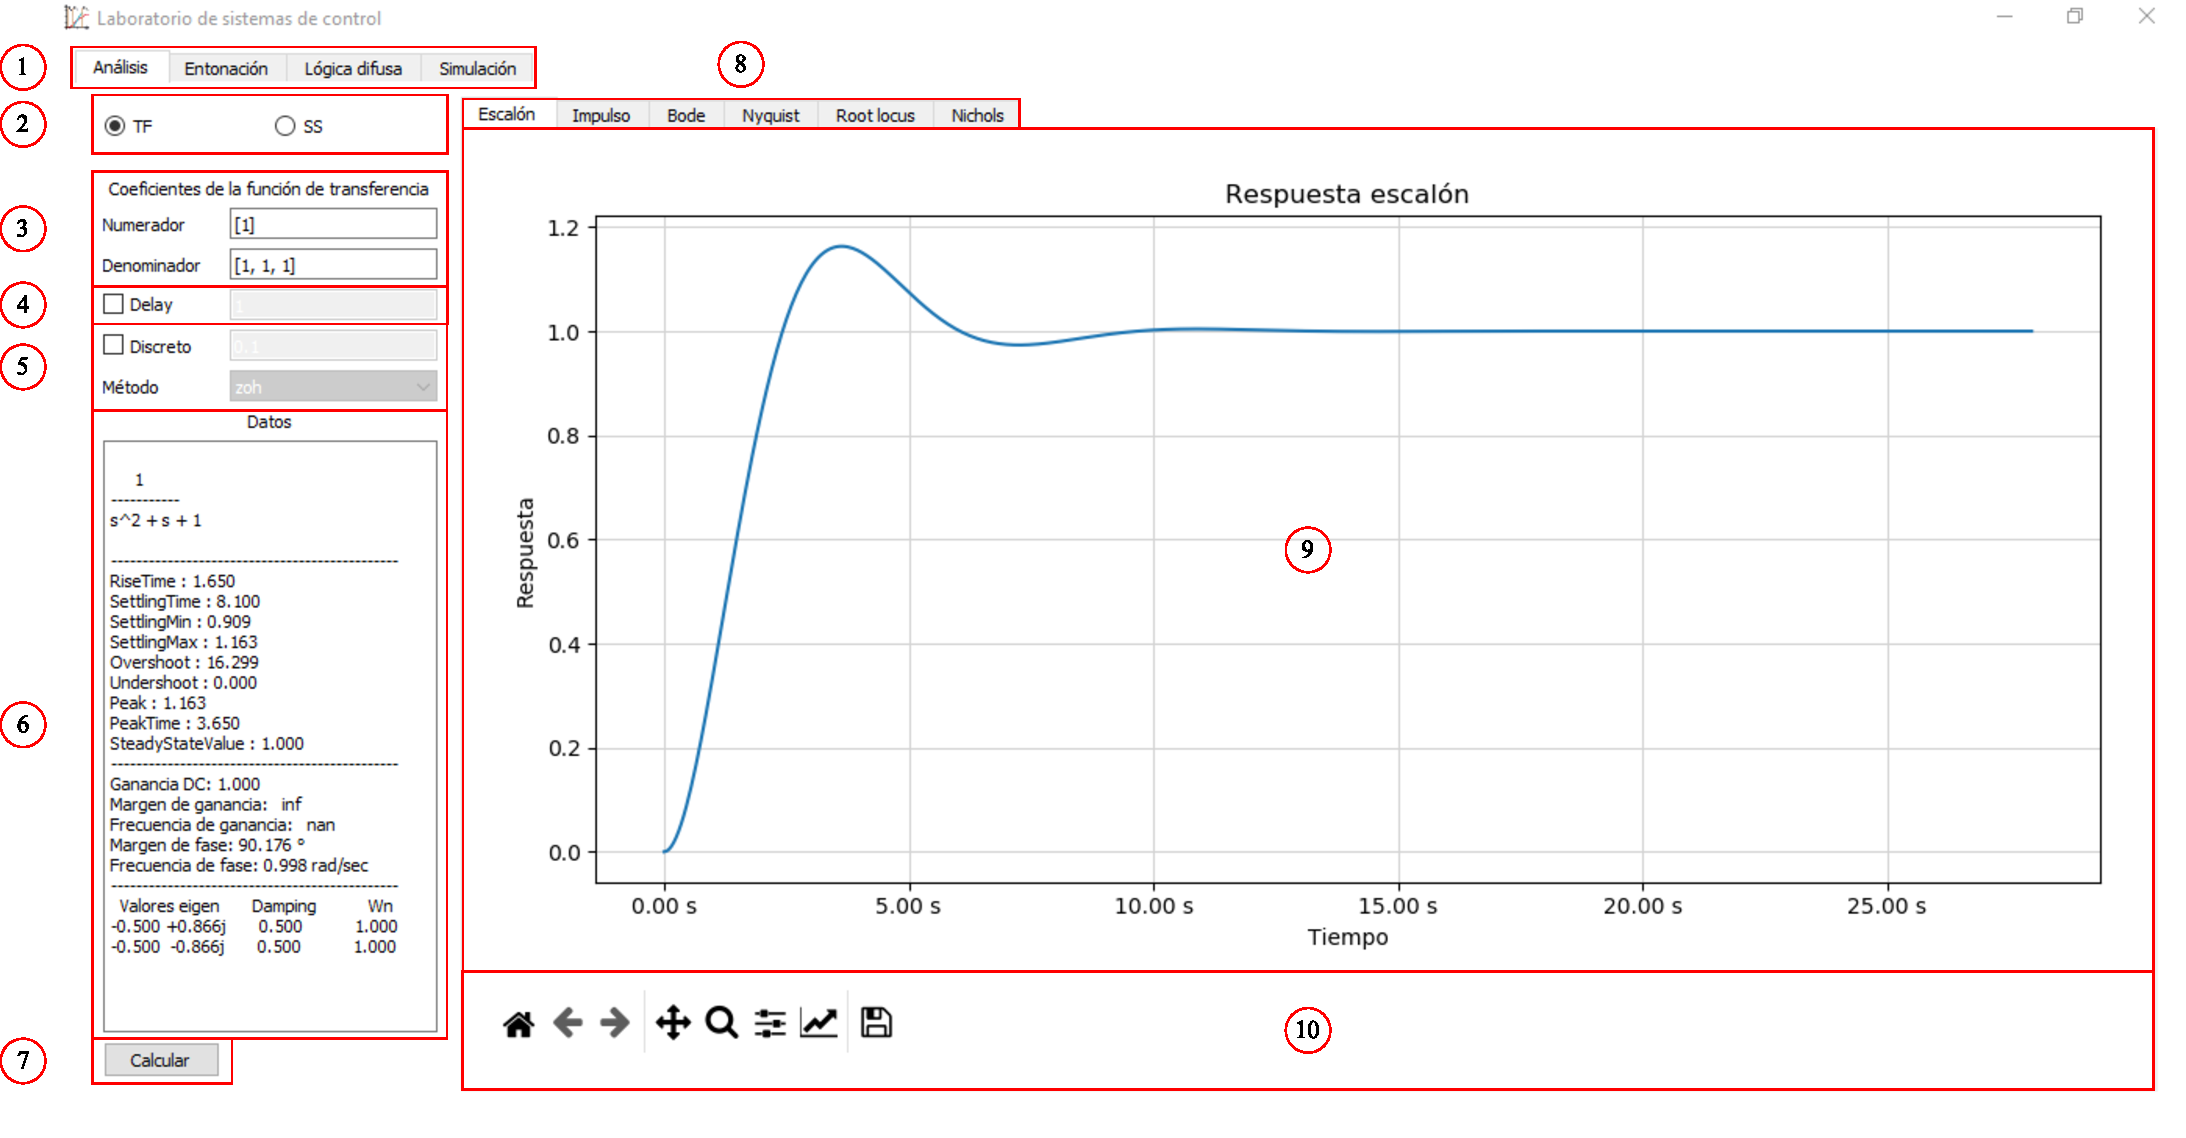
\includegraphics[width=\textwidth]{analisis.pdf}
            \caption{}
            \label{fig:interfazAnalisistf}
        \end{subfigure}
        \hfill
        \begin{subfigure}[t]{0.25\textwidth}
            \centering
            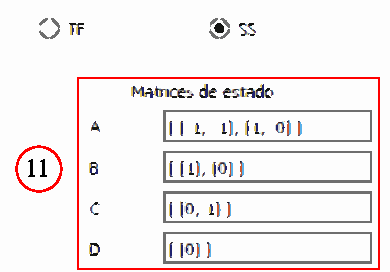
\includegraphics[width=\textwidth]{analisisSS.pdf}
            \caption{}
            \label{fig:interfazAnalisisSS}
        \end{subfigure}
        \caption[Interfaz gráfica para el análisis de sistemas de control]{\textbf{Interfaz gráfica para el análisis de sistemas de control}. (a) Interfaz gráfica general representando al sistema con función de transferencia, (b) Cambios presentes si utiliza la representación con ecuaciones de espacio de estados. Fuente: Elaboración propia. \label{fig:interfazAnalisis}}
    \end{figure}

    \begin{multicols}{2}
        \begin{enumerate}[leftmargin=20pt]
            \item Pestañas de funciones
            \item Selector de representación
            \item Coeficientes de la función de transferencia
            \item Agregado de Delay
            \item Discretización del proceso
            \item Datos del análisis
            \item Botón para realizar el análisis
            \item Pestañas de gráficas
            \item Gráfica con Matplotlib
            \item Barra de herramientas de la gráfica
            \item Matrices de estados
        \end{enumerate}
    \end{multicols}

\AgregarAnexo{Interfaz gráfica de la función de entonación de controladores PID}{anexo:interfazentonacion}
    \begin{figure}[h!]
        \centering
        \begin{subfigure}[t]{\textwidth}
            \centering
            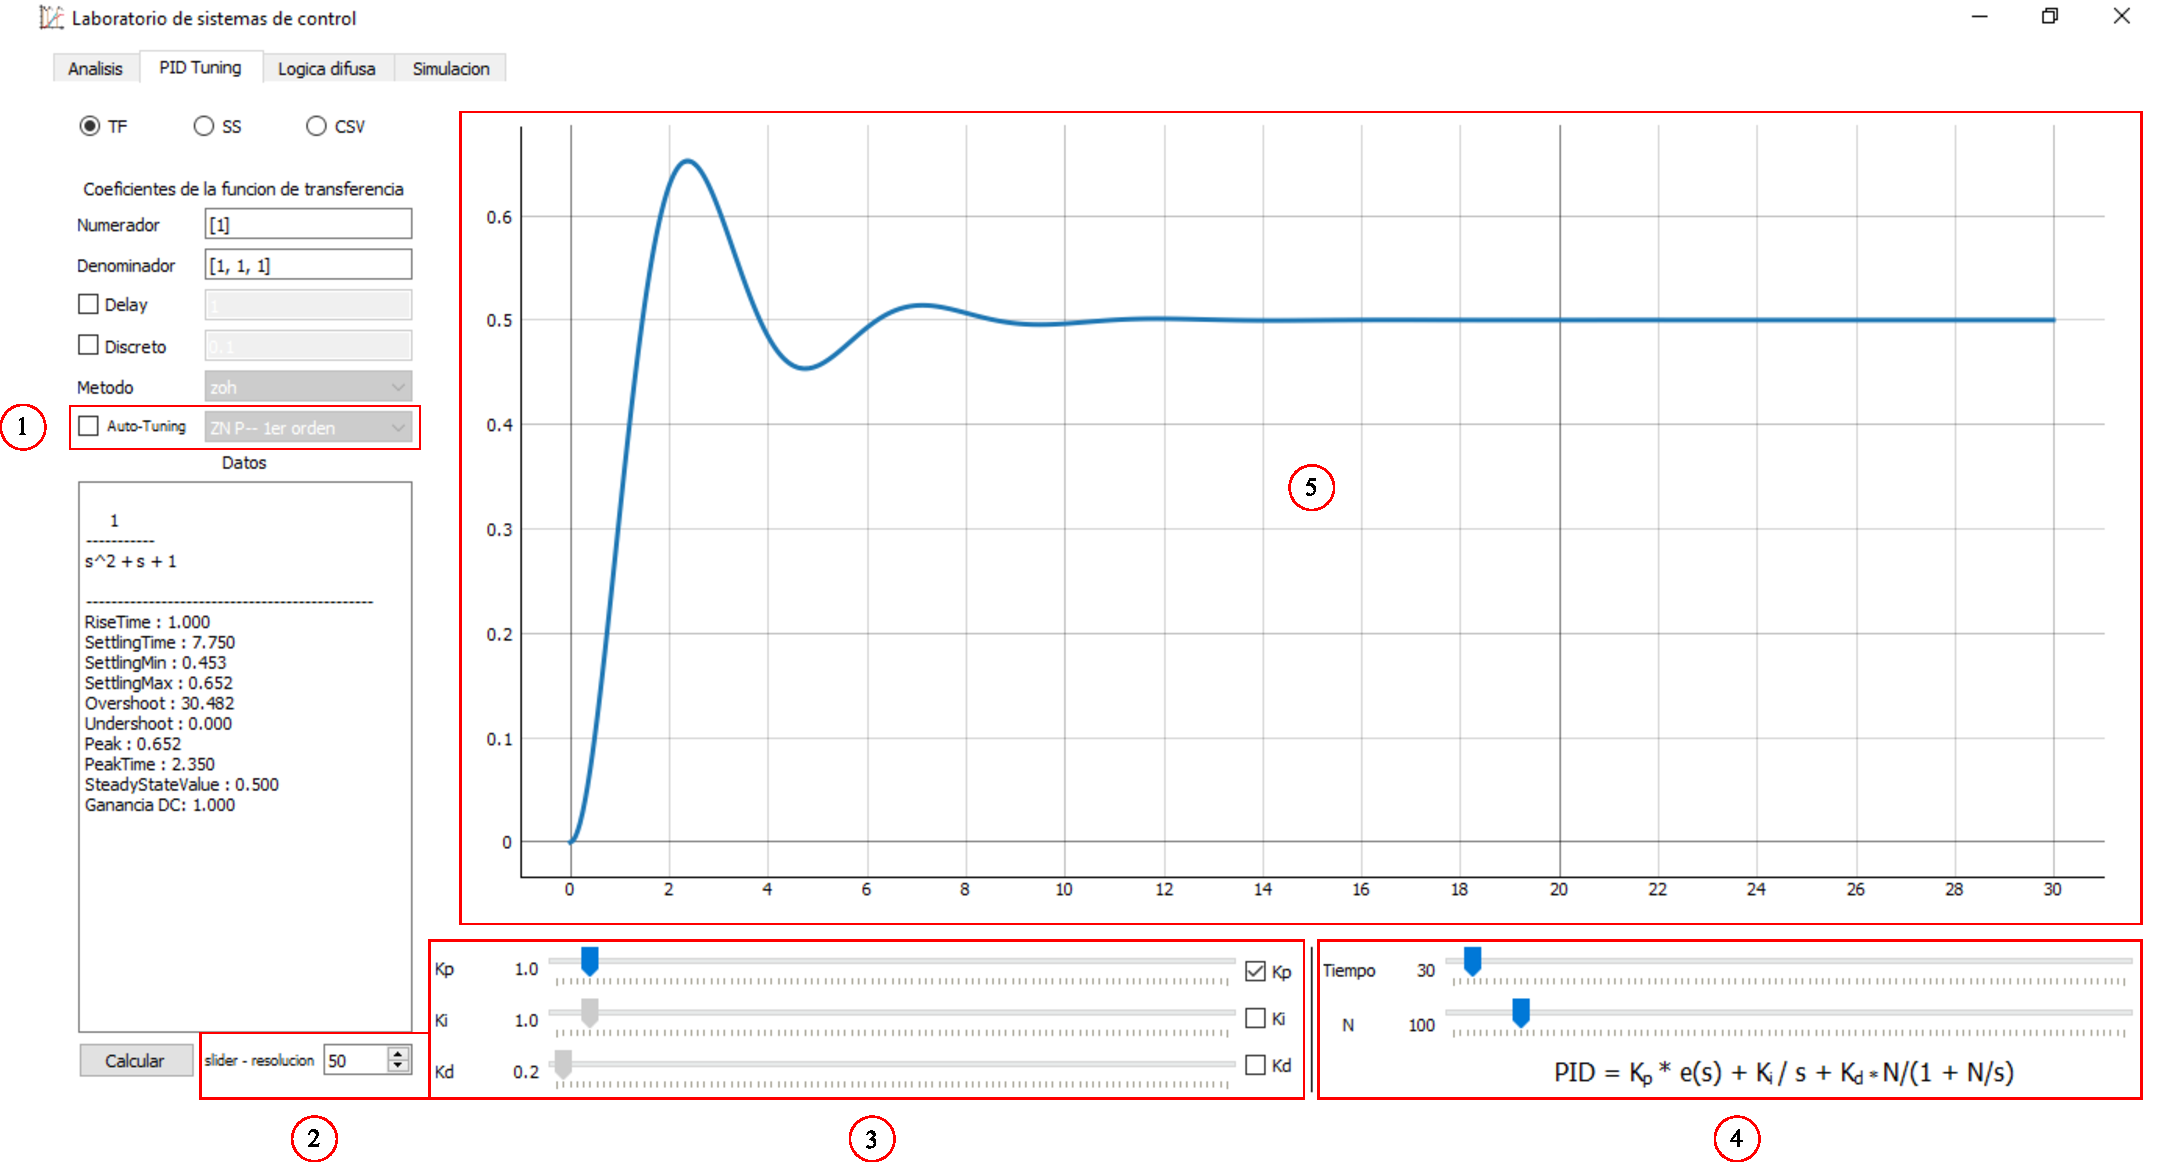
\includegraphics[width=\textwidth]{entonacionPID.pdf}
            \caption{}
            \label{fig:interfazentonacionPID}
        \end{subfigure}
        \hfill
        \begin{subfigure}[t]{\textwidth}
            \centering
            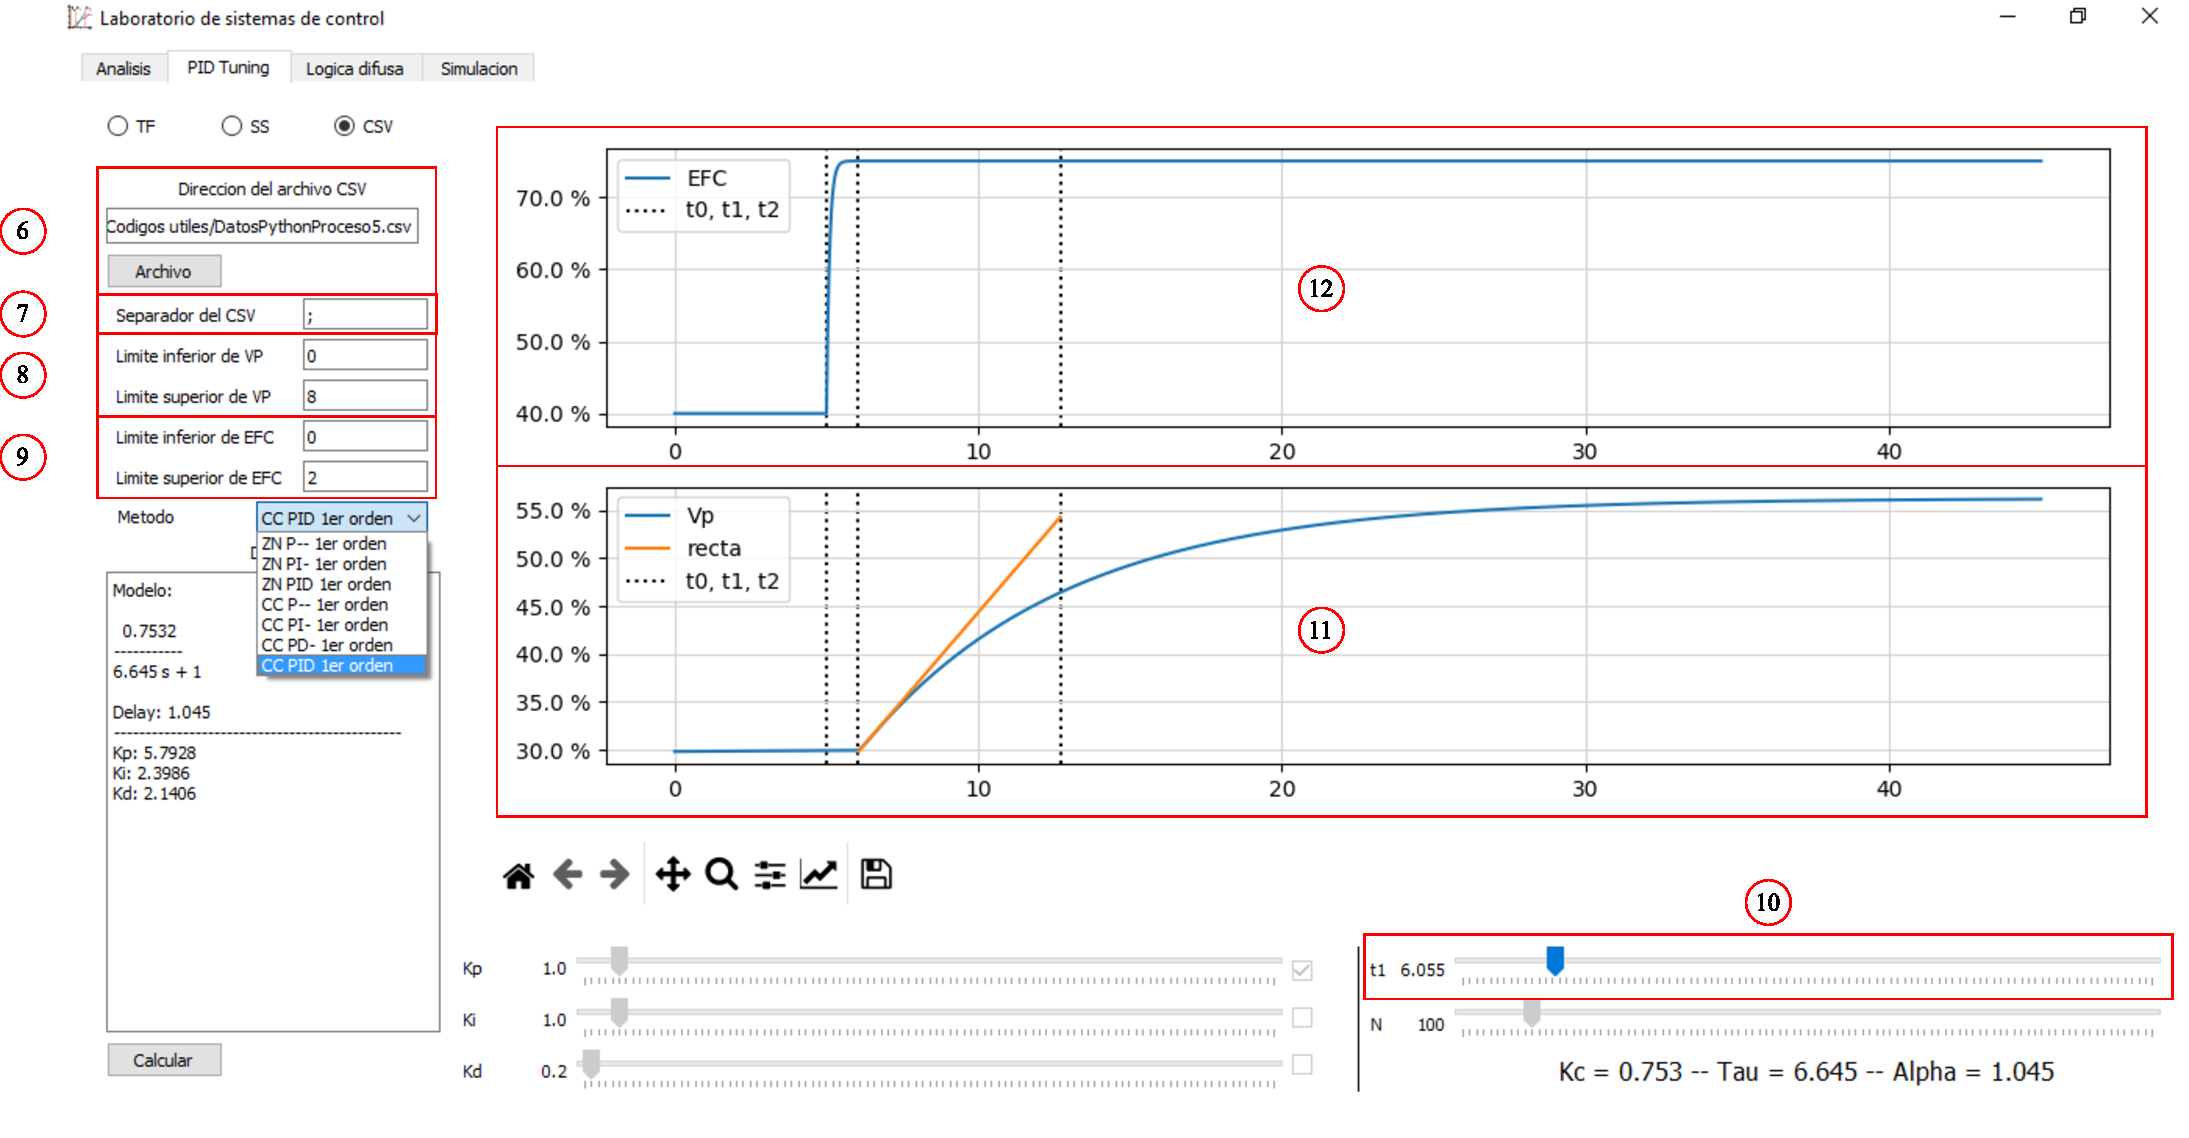
\includegraphics[width=\textwidth]{entonacionCSV.pdf}
            \caption{}
            \label{fig:interfazentonacionCSV}
        \end{subfigure}
        \caption[Interfaz gráfica para la entonación de controladores PID]{\textbf{Interfaz gráfica para la entonación de controladores PID}. (a) Interfaz gráfica general para la entonación de controladores PID, (b) Interfaz gráfica para la entonación utilizando un archivo CSV. Fuente: Elaboración propia. \label{fig:interfazentonacion}}
    \end{figure}

    \begin{multicols}{2}
        \begin{enumerate}[leftmargin=20pt]
            \item Función de entonación automática
            \item Resolución de los sliders
            \item Sliders de ganancias
            \item Sliders de tiempo y coeficiente N
            \item Gráfica con PyQtGraph
            \item Carga del archivo CSV
            \item Separador del archivo CSV
            \item SPAN de la variable del proceso
            \item SPAN de la entrada al proceso (EFC)
            \item Slider para ajustar $t_1$
            \item Gráfica de la variable del proceso
            \item Gráfica de la entrada al proceso (EFC)
        \end{enumerate}
    \end{multicols}

\AgregarAnexo{Interfaz gráfica de la función de diseño de controladores difusos}{anexo:interfazFuzzy}
    
    \vfill
    
    \begin{figure}[htb]
        \centering
        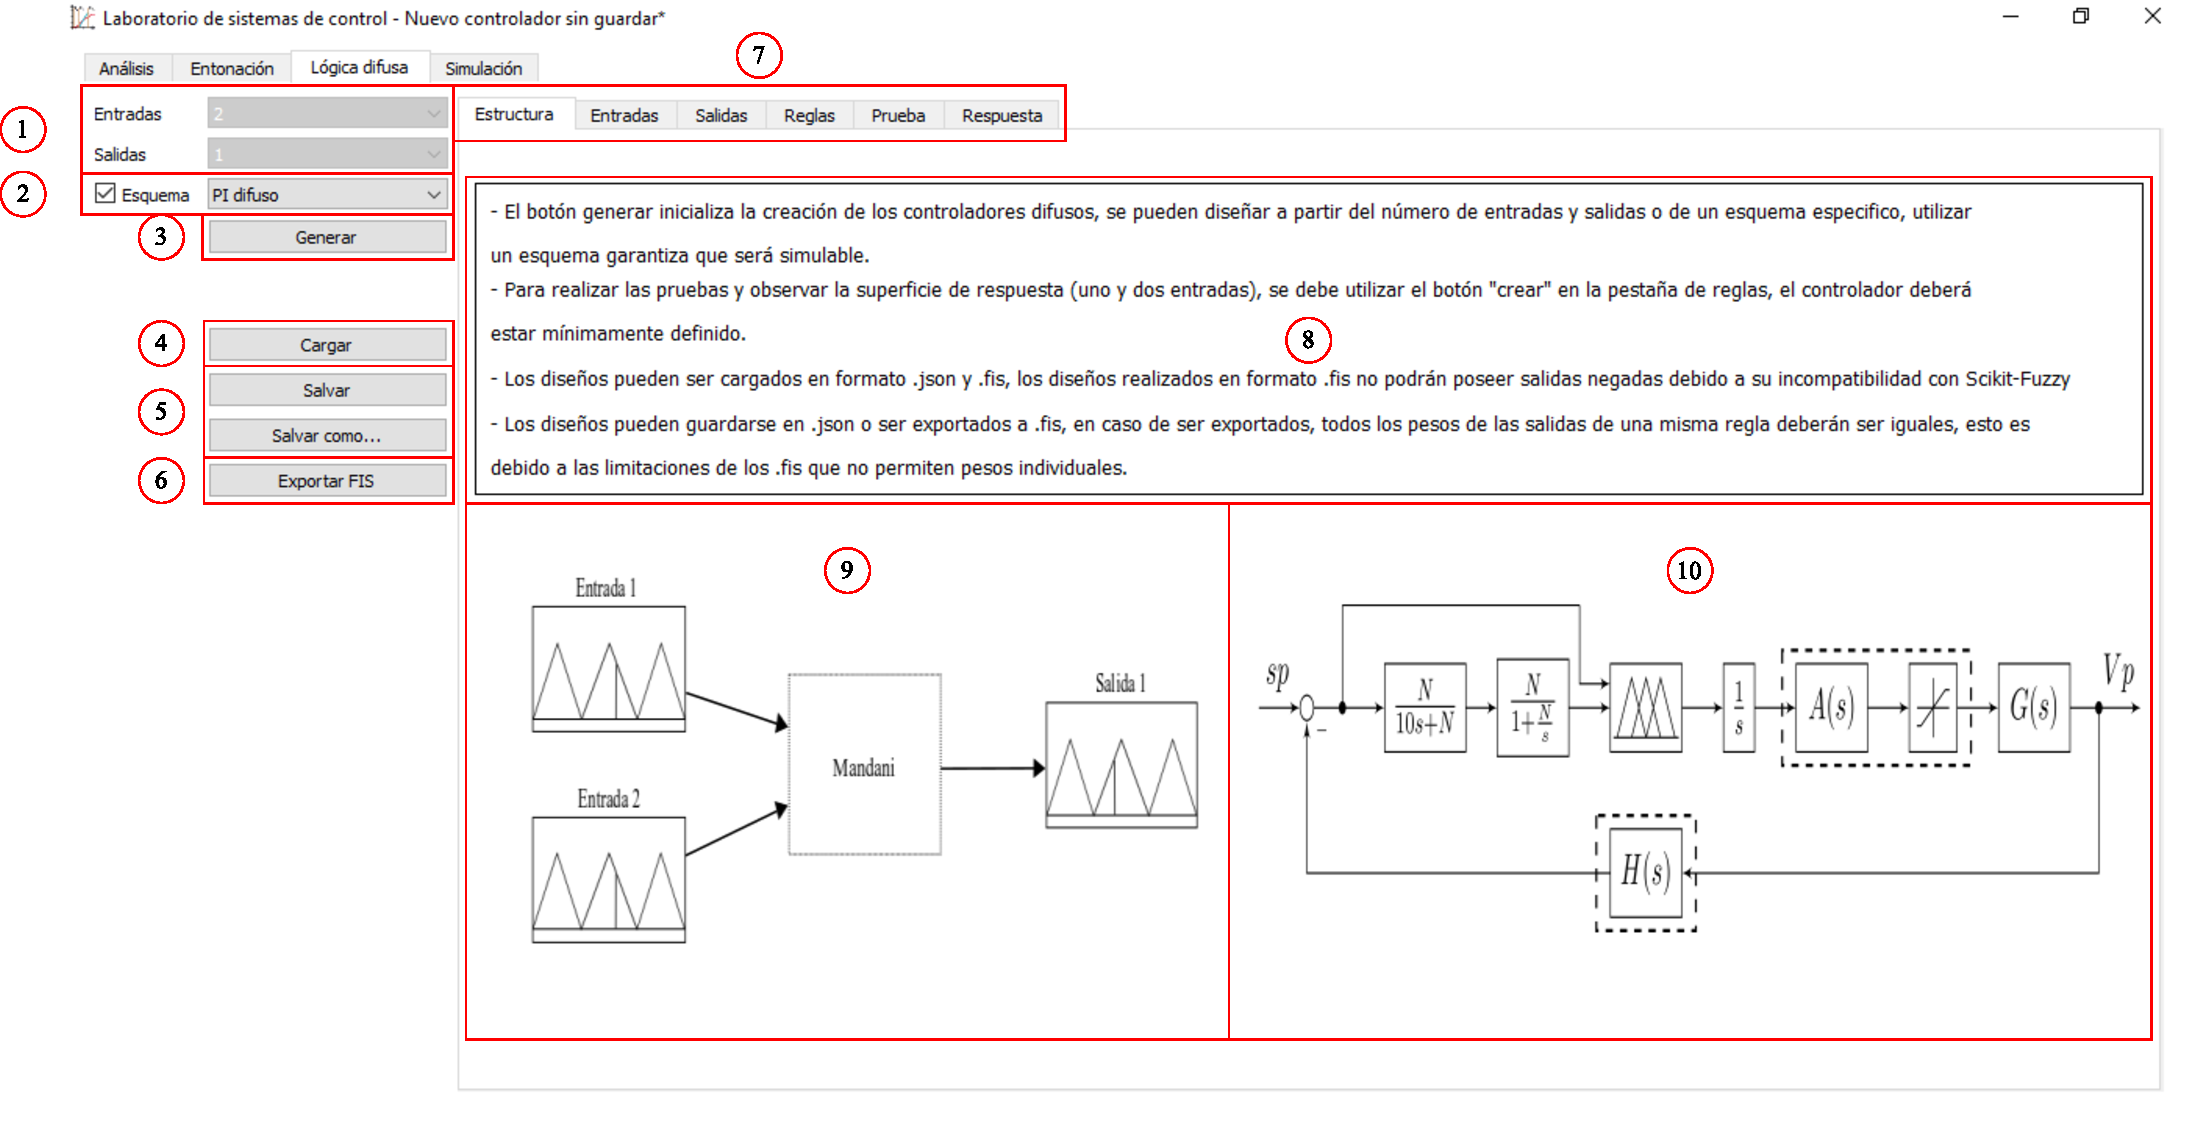
\includegraphics[width=\textwidth]{FuzzyFront.pdf}
        \caption[Interfaz gráfica - difusa - estructura]{\textbf{Interfaz gráfica - difusa}. Pestaña de estructura. Fuente: Elaboración propia.} 
        \label{fig:FuzzyFront}
    \end{figure}
    
    \vfill

    \begin{multicols}{2}
        \begin{enumerate}[leftmargin=20pt]
            \item Número de entradas y salidas
            \item Selección de esquema de control
            \item Botón para iniciar el diseño
            \item Botón para cargar un diseño
            \item Botones para salvar los diseños
            \item Botón para exportar el diseño a FIS
            \item Pestañas para el diseño
            \item Información general
            \item Estructura de entradas y salidas
            \item Esquema de control
        \end{enumerate}
    \end{multicols}

    \vfill

    \pagebreak
    
    \begin{figure}[htb]
        \centering
        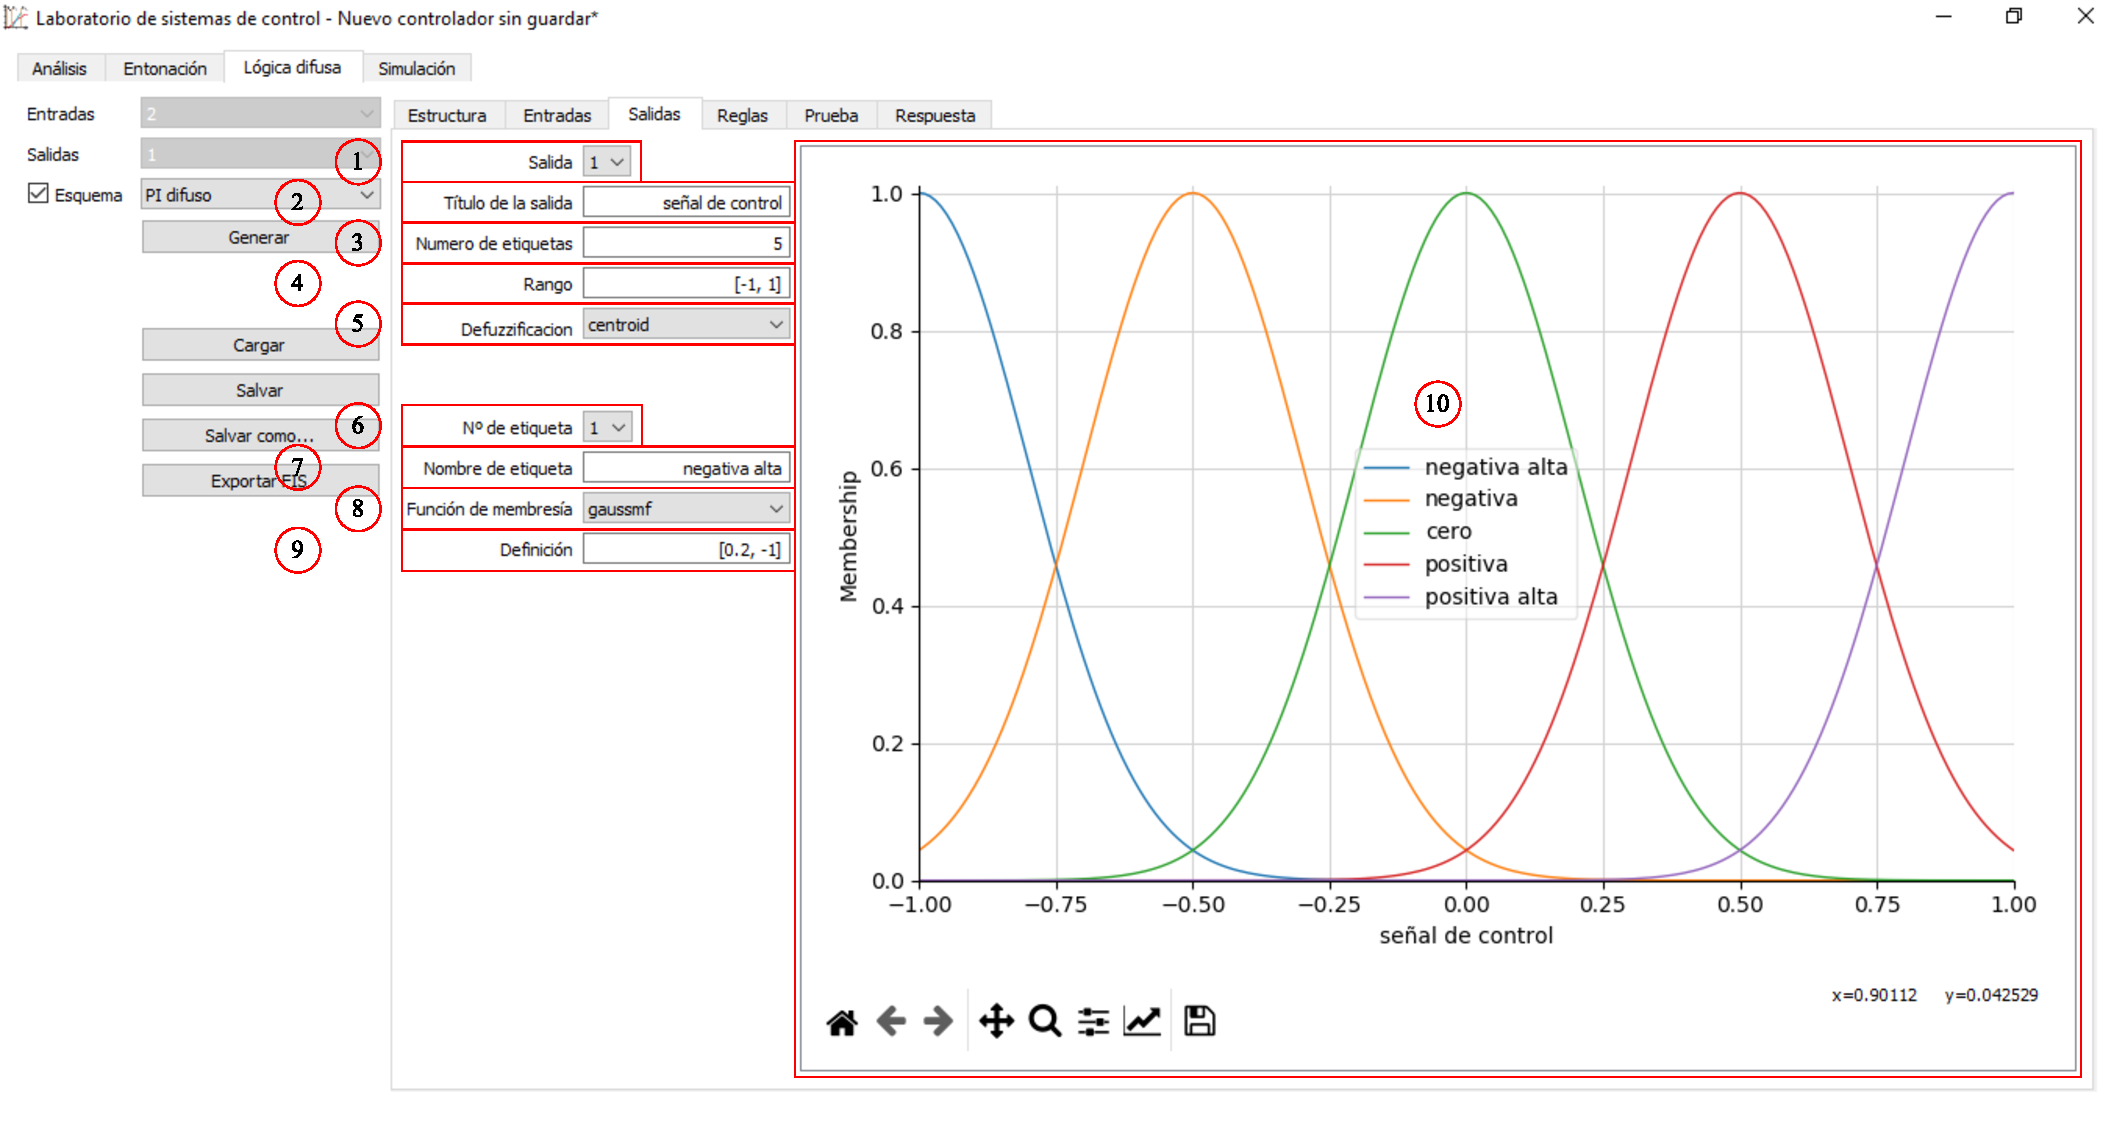
\includegraphics[width=0.9\textwidth]{FuzzyIO.pdf}
        \caption[Interfaz gráfica - difusa - entradas/salidas]{\textbf{Interfaz gráfica - difusa}. Pestaña de salidas, la única diferencia respecto a la pestaña de entradas es que esta segunda no posee método de defuzzificacion. Fuente: Elaboración propia.} 
        \label{fig:FuzzyIO}
    \end{figure}

    \begin{multicols}{2}
        \begin{enumerate}[leftmargin=20pt]
            \item Número de entrada/salida
            \item Nombre de la entrada/salida
            \item Número de etiquetas
            \item Rango de la entrada/salida
            \item Método de defuzzificacion
            \item Número de etiqueta
            \item Nombre de la etiqueta
            \item Tipo de función de membresía
            \item Definición de la función de membresía
            \item Gráfica de las funciones de membresía
        \end{enumerate}
    \end{multicols}

    \begin{figure}[!h]
        \centering
        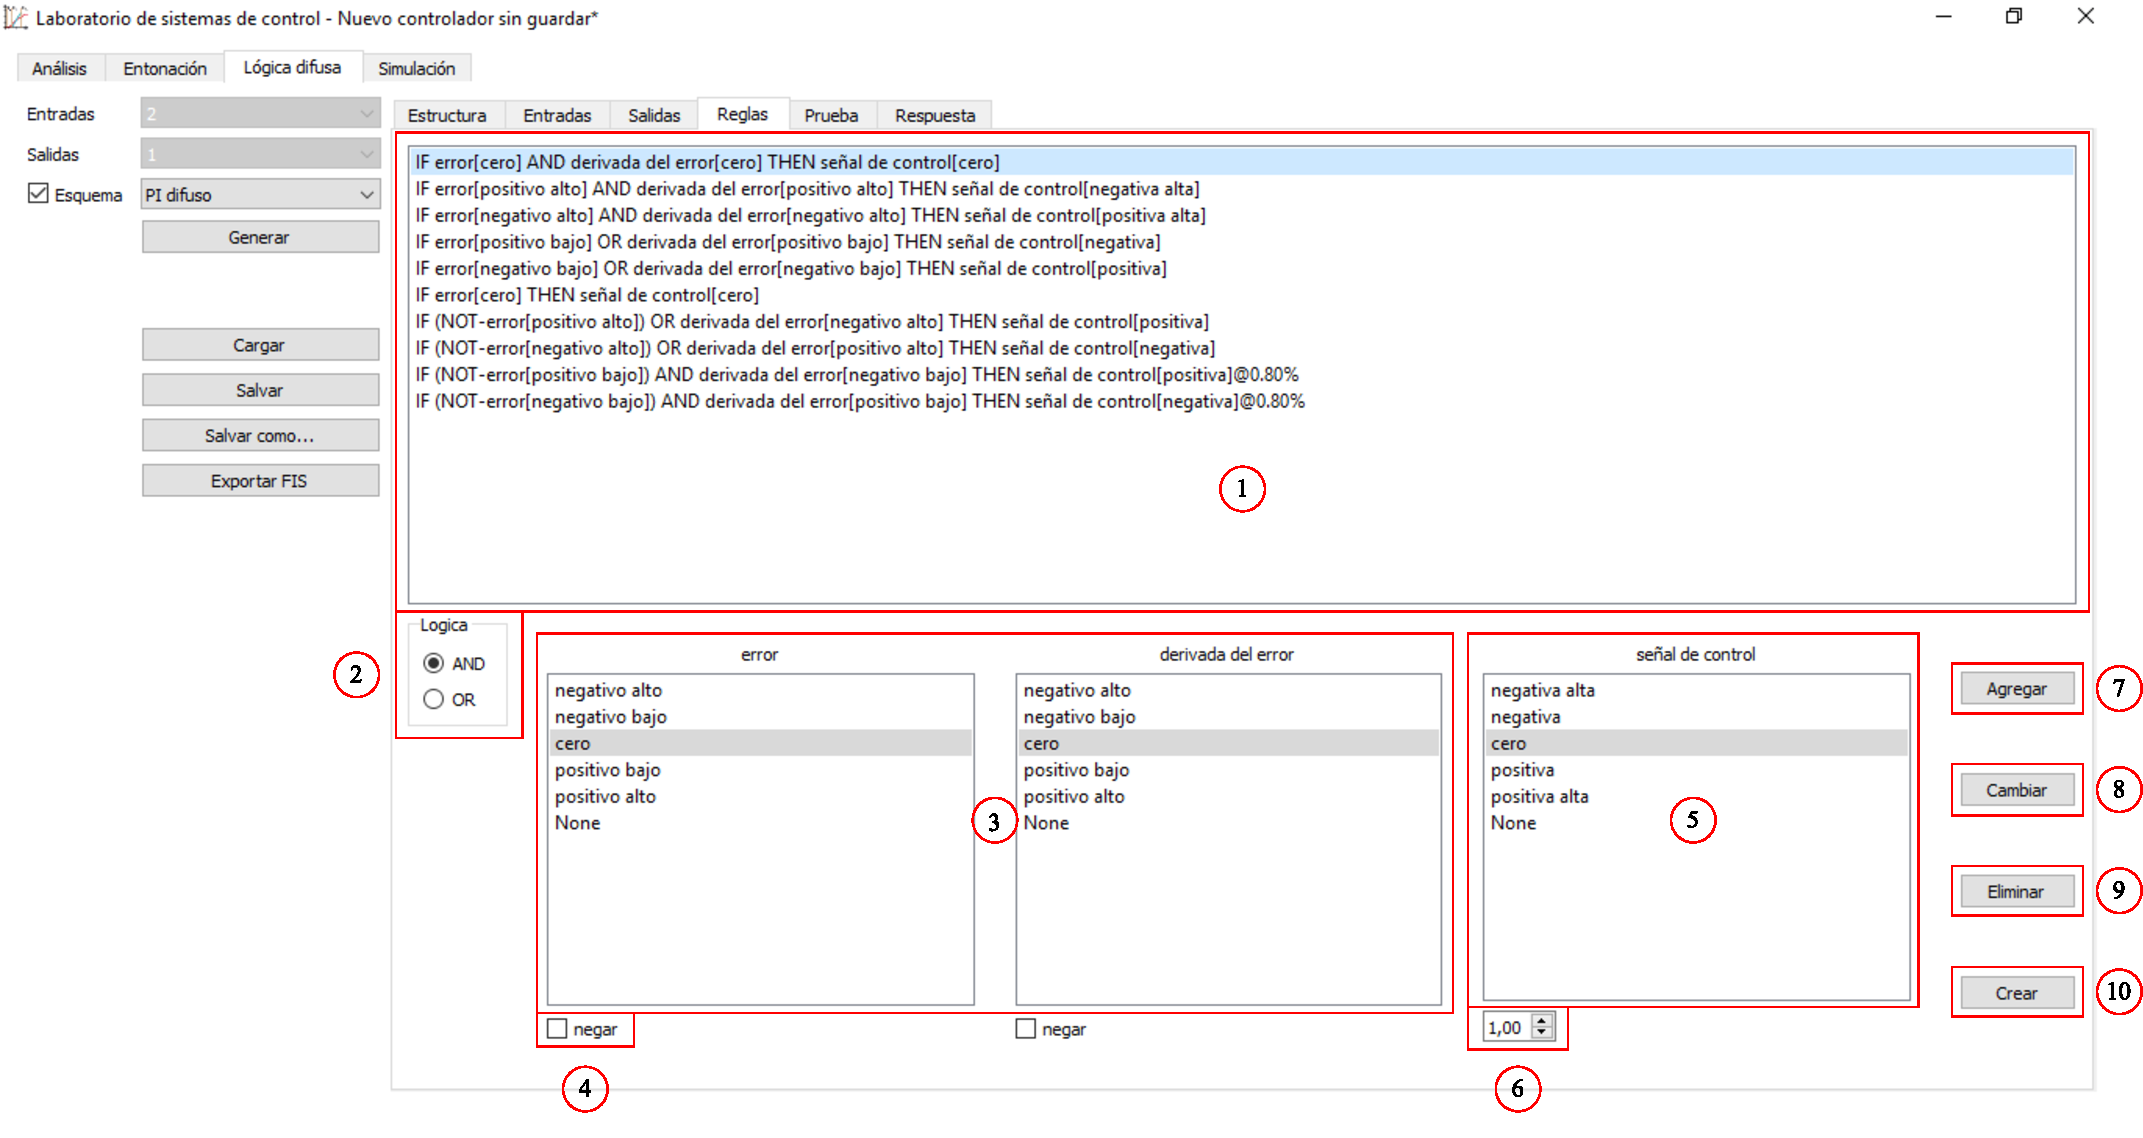
\includegraphics[width=0.9\textwidth]{FuzzyRules.pdf}
        \caption[Interfaz gráfica - difusa - reglas]{\textbf{Interfaz gráfica - difusa}. Pestaña de reglas. Fuente: Elaboración propia.} 
        \label{fig:FuzzyRules}
    \end{figure}

    \begin{multicols}{2}
        \begin{enumerate}[leftmargin=20pt]
            \item Lista de reglas
            \item Lógica de las premisas
            \item Etiquetas de las entradas
            \item Opción para negar la entrada
            \item Etiquetas de las salidas
            \item Peso de la salida
            \item Botón para agregar una regla
            \item Botón para cambiar una regla
            \item Botón para eliminar una regla
            \item Botón para crear el controlador y realizar pruebas
        \end{enumerate}
    \end{multicols}

    \begin{figure}[h!]
        \centering
        \begin{subfigure}[t]{\textwidth}
            \centering
            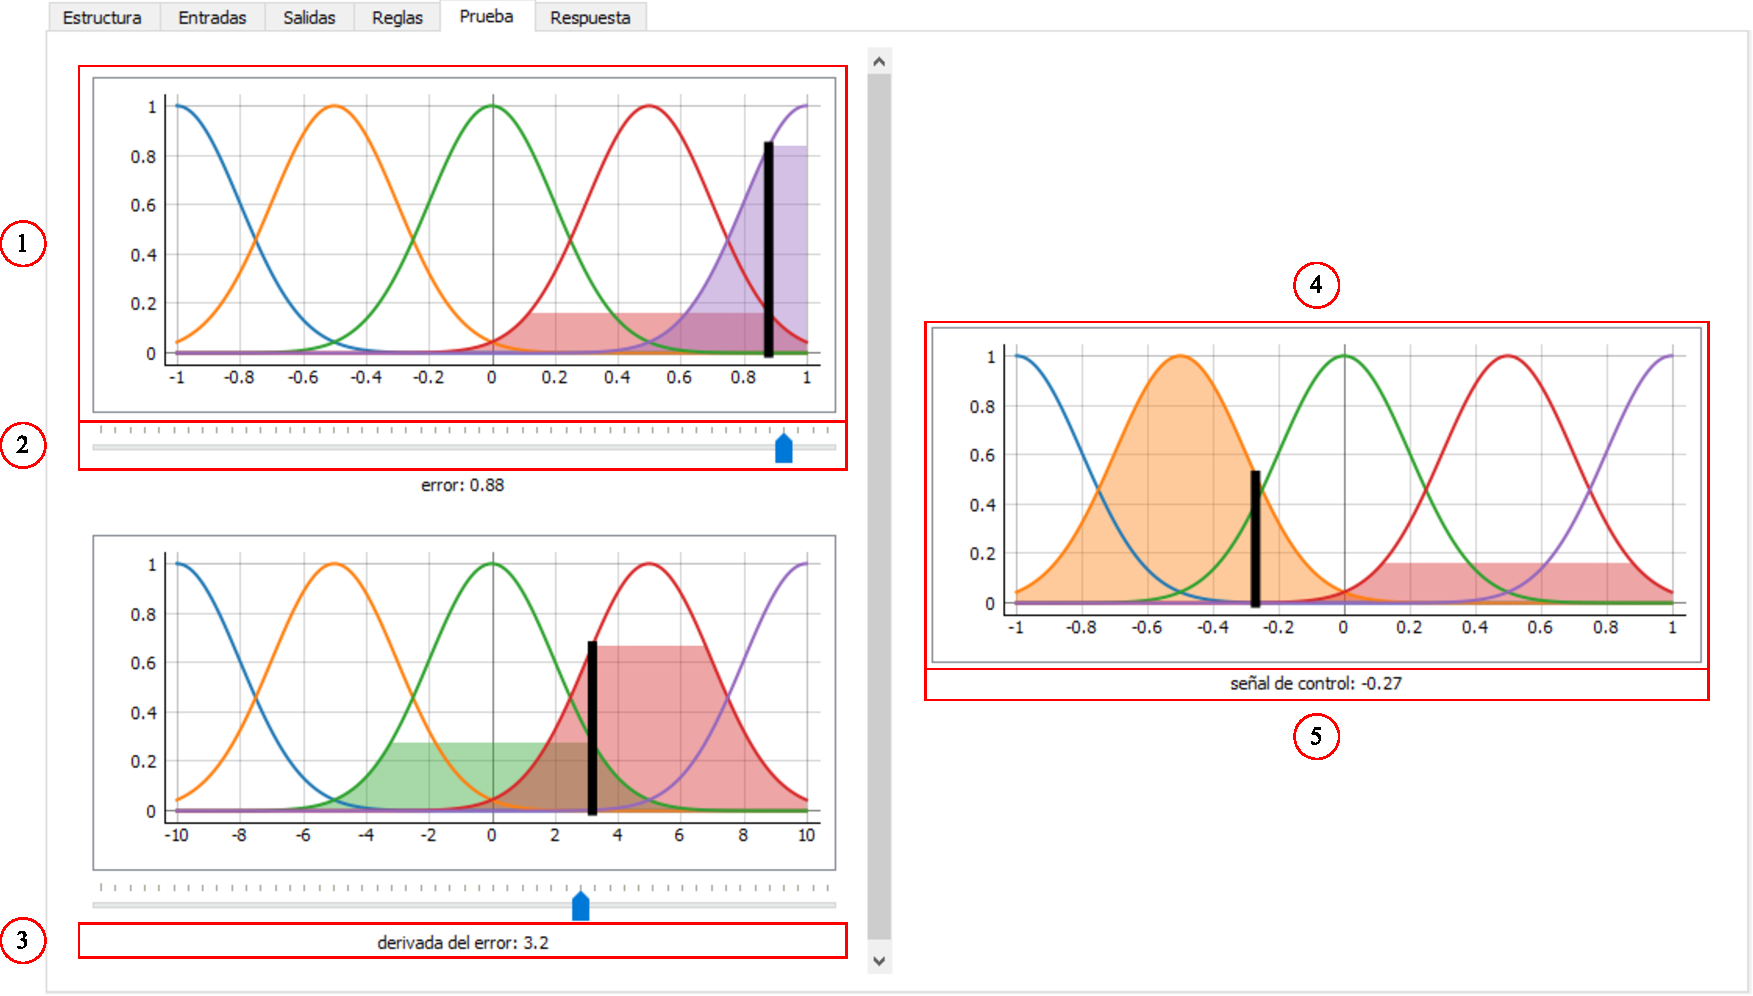
\includegraphics[width=0.75\textwidth]{FuzzyPrueba.pdf}
            \caption{}
            \label{fig:FuzzyPrueba}
        \end{subfigure}
        \hfill
        \begin{subfigure}[t]{\textwidth}
            \centering
            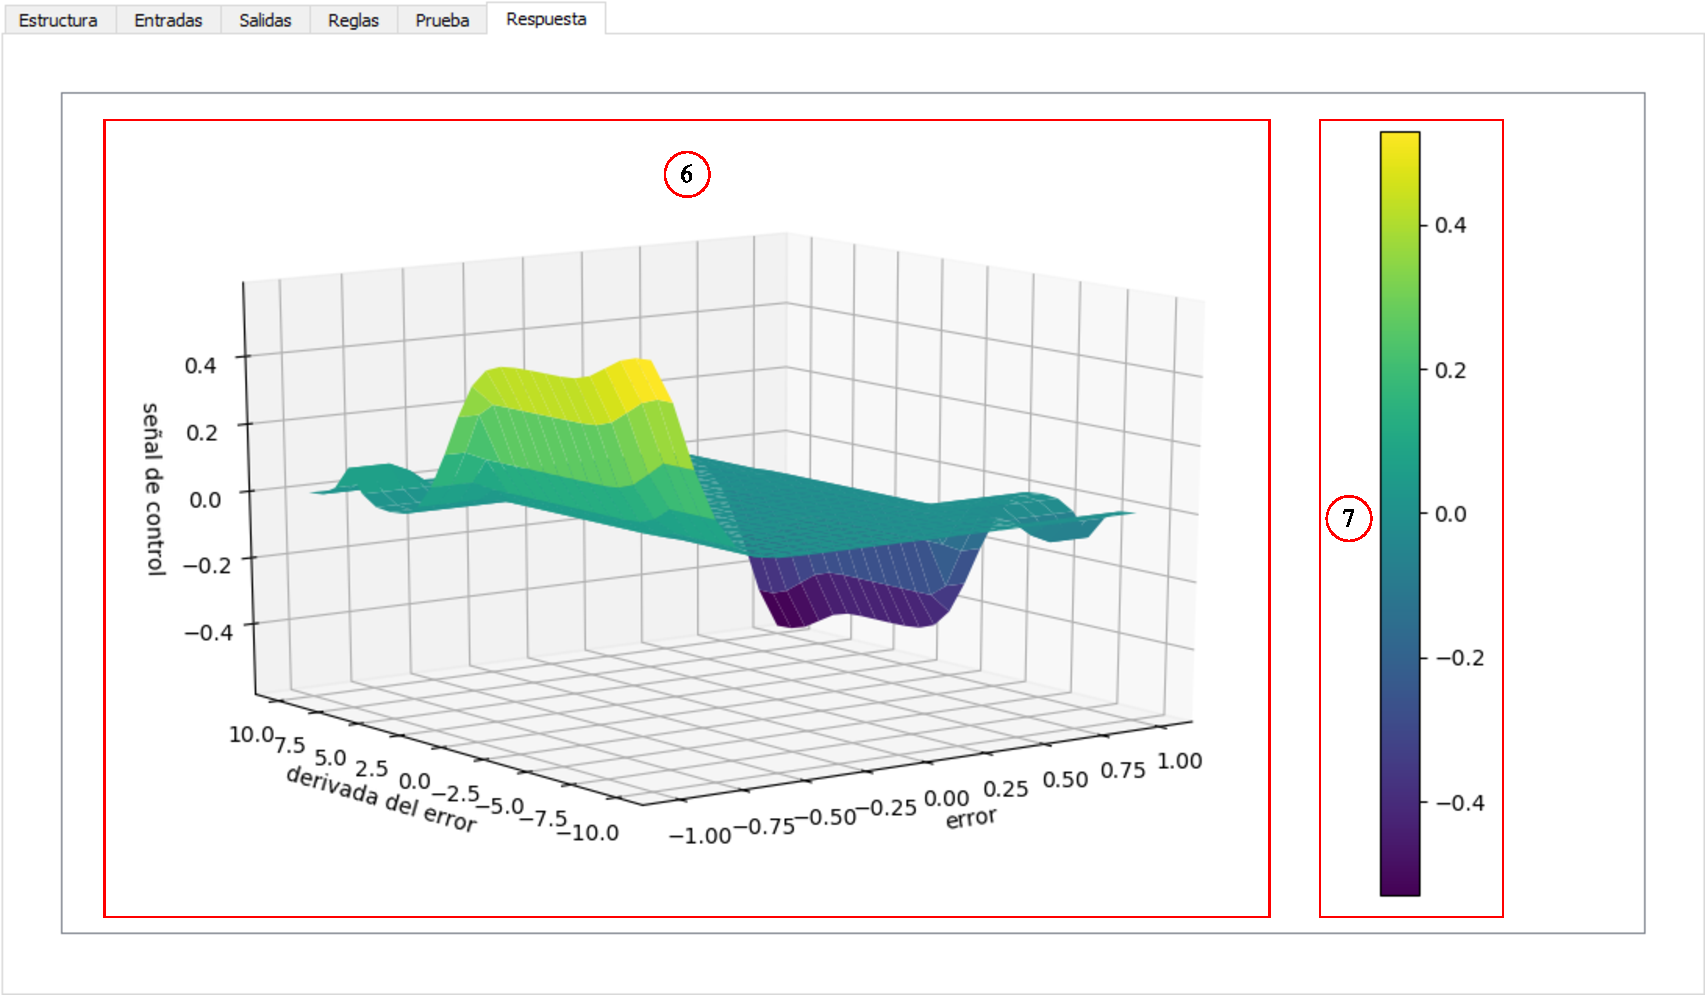
\includegraphics[width=0.75\textwidth]{FuzzyRespuesta.pdf}
            \caption{}
            \label{fig:FuzzyRespuesta}
        \end{subfigure}
        \caption[Interfaz gráfica - difusa - prueba y respuesta]{\textbf{Interfaz gráfica - difusa}. (a) Pestaña para pruebas del controlador, (b) Pestaña para observar la respuesta del controlador, solo visible para controladores con una o dos entradas. Fuente: Elaboración propia. \label{fig:interfazFuzzyCrear}}
    \end{figure}

    \begin{multicols}{2}
        \begin{enumerate}[leftmargin=20pt]
            \item Activación de reglas de forma gráfica para las entradas
            \item Slider para asignar entrada
            \item Valor de entrada
            \item Activación de reglas de forma gráfica para las salidas
            \item Valor de salida
            \item Respuesta del controlador
            \item Barra indicadora de altura (para dos entradas)
        \end{enumerate}
    \end{multicols}

\AgregarAnexo{Interfaz gráfica para la simulación de sistemas de control}{anexo:interfazSimulacion}

    \begin{figure}[h!]
        \centering
        \begin{subfigure}[t]{\textwidth}
            \centering
            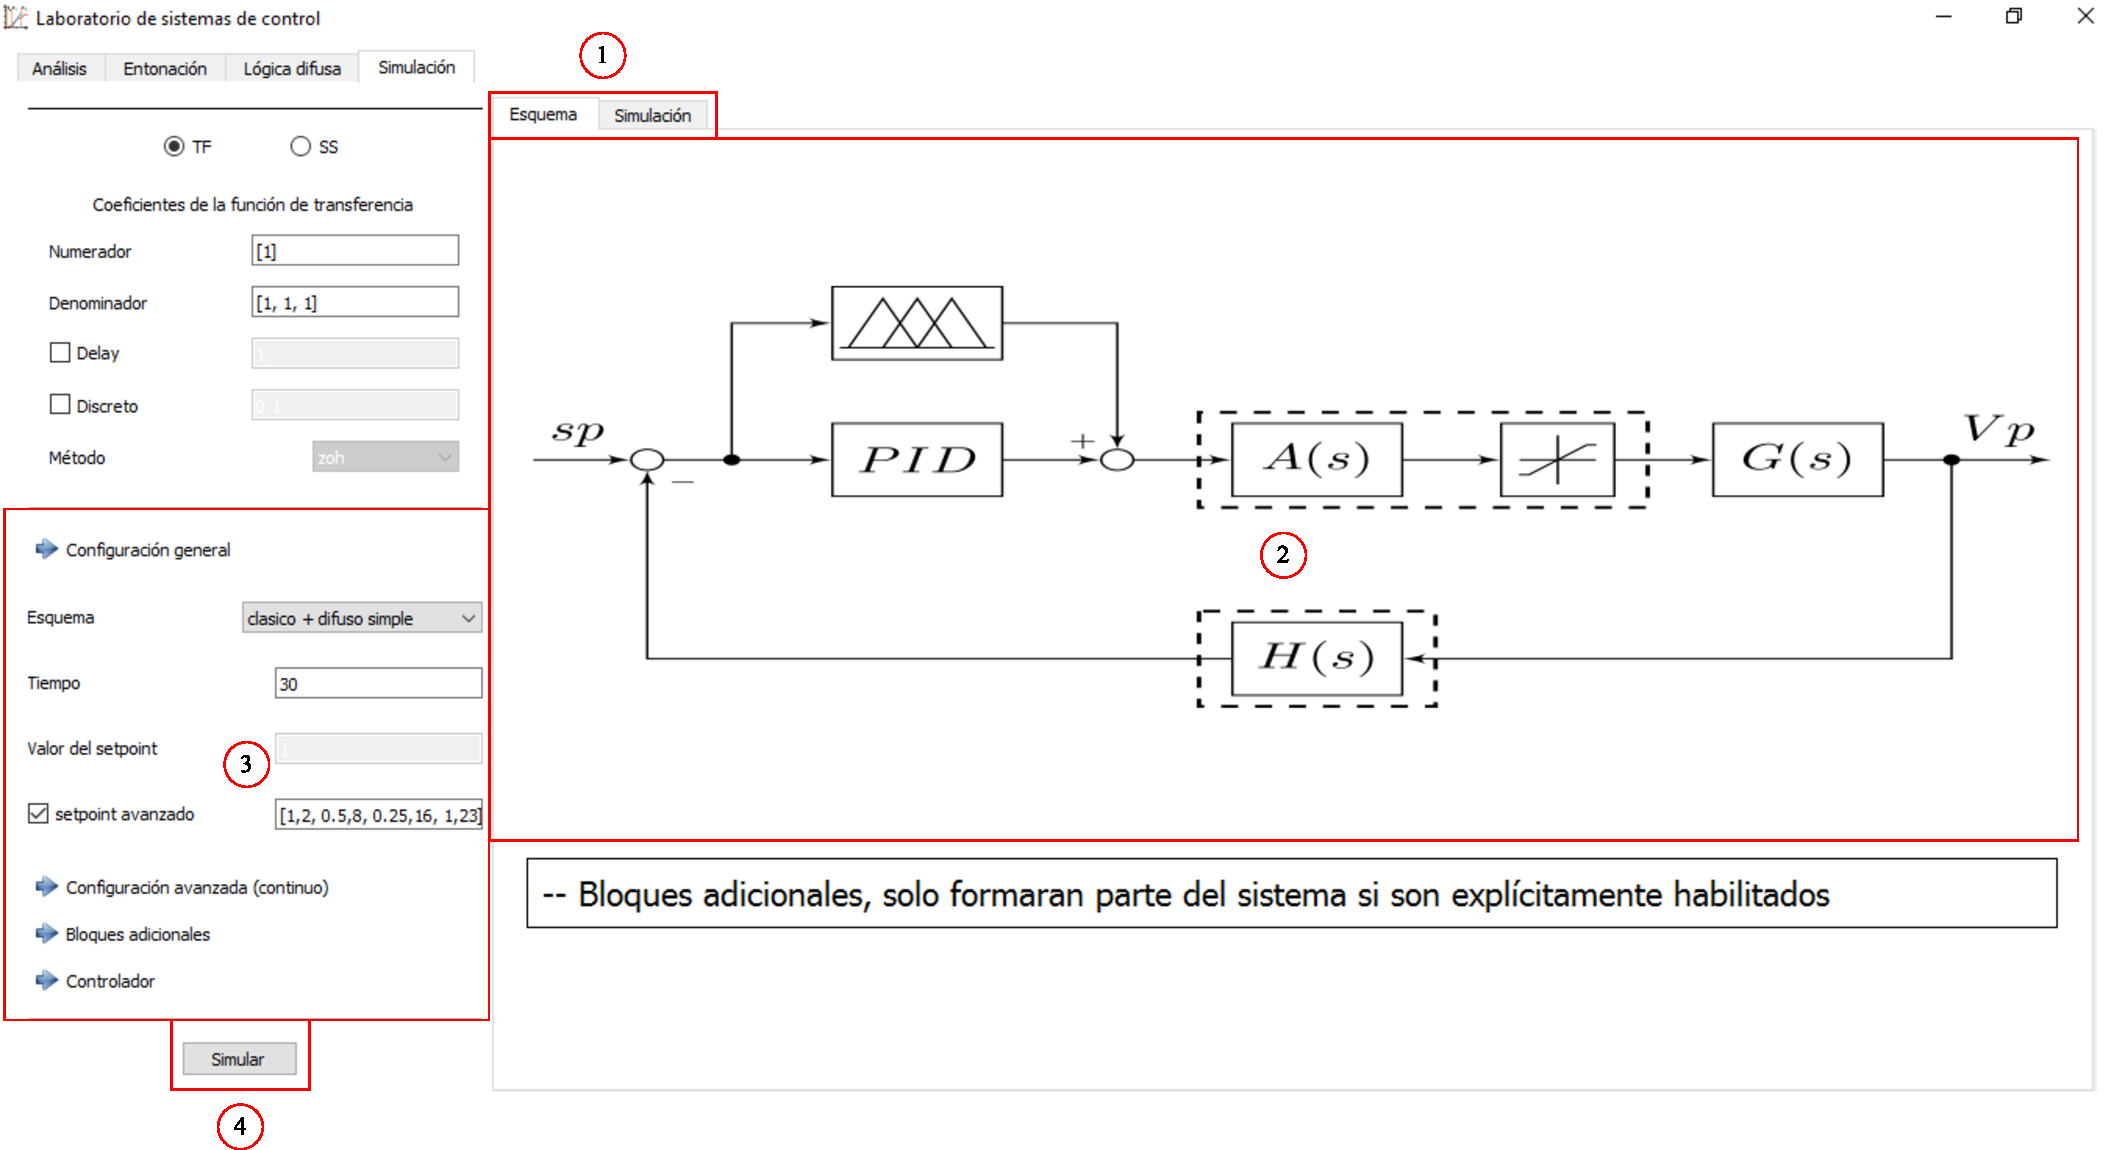
\includegraphics[width=0.8\textwidth]{SimulacionGeneral.pdf}
            \caption{}
            \label{fig:SimulacionGeneral}
        \end{subfigure}
        \hfill
        \begin{subfigure}[t]{\textwidth}
            \centering
            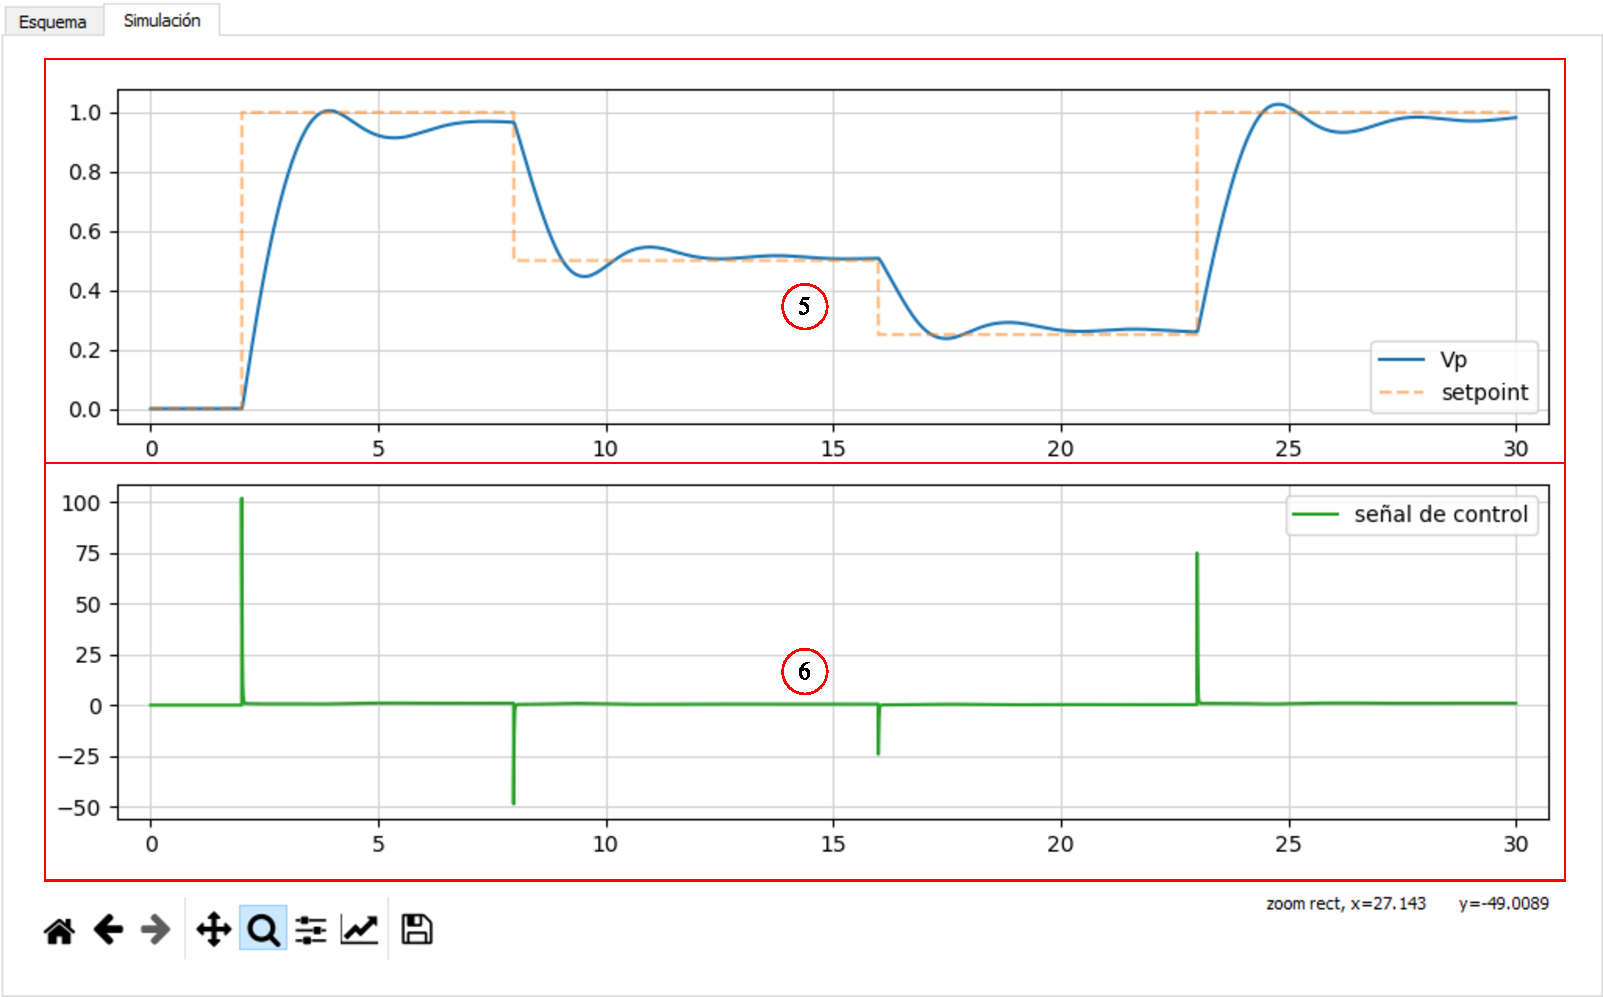
\includegraphics[width=0.8\textwidth]{SimulacionPlot.pdf}
            \caption{}
            \label{fig:SimulacionPlot}
        \end{subfigure}
        \caption[Interfaz gráfica para la simulación de sistemas de control]{\textbf{Interfaz gráfica para la simulación de sistemas de control}. (a) Interfaz gráfica general para la simulación, (b) Pestaña de gráficas de respuesta. Fuente: Elaboración propia. \label{fig:SimulacionFront}}
    \end{figure}

    \begin{multicols}{2}
        \begin{enumerate}[leftmargin=20pt]
            \item Pestañas de simulación
            \item Esquema de control
            \item Barras de configuración
            \item Botón para simular
            \item Gráfica de respuesta del sistema
            \item Gráfica de la señal de control
        \end{enumerate}
    \end{multicols}

    \begin{figure}[h]
        \centering
        \begin{subfigure}[b]{0.49\textwidth}
            \centering
            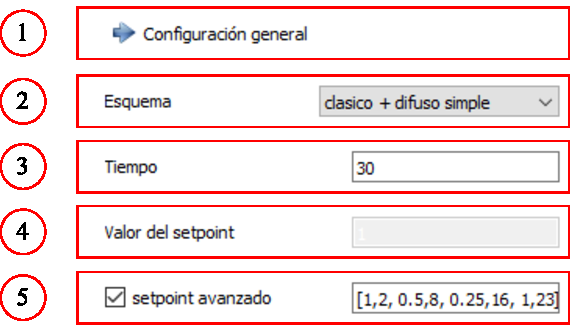
\includegraphics[width=\textwidth]{ConfGeneral.pdf}
            \caption{}
            \label{fig:ConfGeneral}
        \end{subfigure}
        \hfill
        \begin{subfigure}[b]{0.49\textwidth}
            \centering
            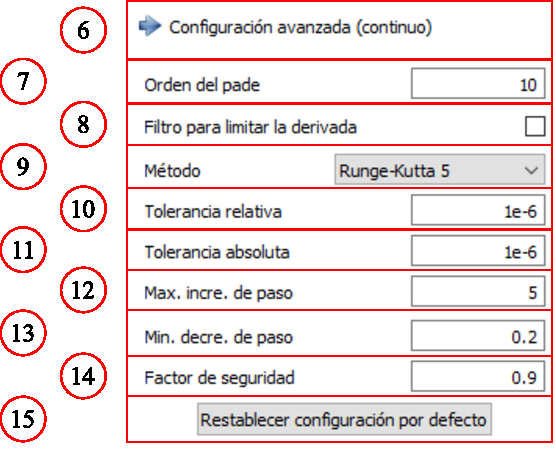
\includegraphics[width=\textwidth]{ConfAvz.pdf}
            \caption{}
            \label{fig:ConfAvz}
        \end{subfigure}
        \hfill
        \begin{subfigure}[b]{0.49\textwidth}
            \centering
            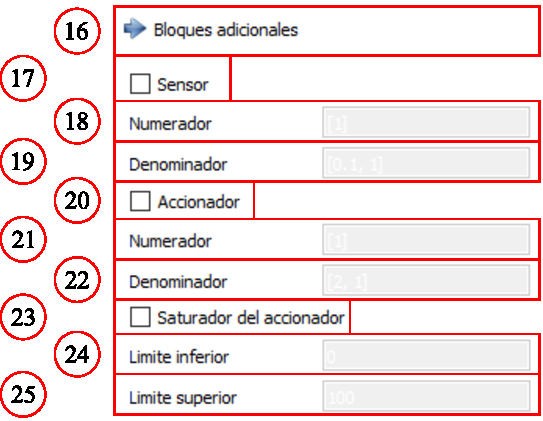
\includegraphics[width=\textwidth]{ConfBloques.pdf}
            \caption{}
            \label{fig:ConfBloques}
        \end{subfigure}
        \hfill
        \begin{subfigure}[b]{0.49\textwidth}
            \centering
            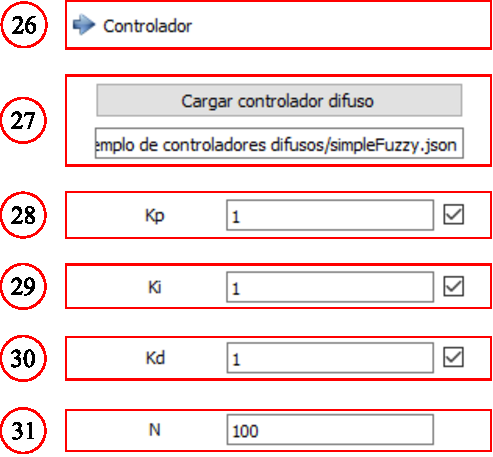
\includegraphics[width=\textwidth]{ConfControlador.pdf}
            \caption{}
            \label{fig:ConfControlador}
        \end{subfigure}
        \caption[Interfaz gráfica - simulación - Barras de configuración]{\textbf{Interfaz gráfica - simulación}. (a) Barra de configuración general, (b) Barra de configuración avanzada, (c) Barra de para agregar bloques adicionales, (d) Barra para configurar los controladores. Fuente: Elaboración propia. \label{fig:SimulacionBarras}}
    \end{figure}

    \begin{multicols}{2}
        \begin{enumerate}[leftmargin=20pt]
            \item Barra de configuración general
            \item Selección del esquema de control
            \item Tiempo de simulación
            \item Valor del setpoint
            \item Setpoint avanzado (variable)
            \item Barra de configuración avanzada
            \item Orden del atraso por PADE
            \item Activación del filtro para la derivada
            \item Selección del método de Runge-Kutta
            \item Tolerancia relativa para el paso variable
            \item Tolerancia absoluta para el paso variable
            \item Máximo incremento del tamaño de paso
            \item Mínimo decremento del tamaño de paso
            \item Factor de seguridad para el paso variable
            \item Botón para reiniciar la configuración
            \item Barra de bloques adicionales
            \item Activación del sensor
            \item Numerador del sensor
            \item Denominador del sensor
            \item Activación del accionador
            \item Numerador del accionador
            \item Denominador del accionador
            \item Activación del saturador
            \item Límite inferior del saturador
            \item Límite superior del saturador
            \item Barra de configuración del controlador
            \item Controlador difuso
            \item Ganancia proporcional del PID
            \item Ganancia integral del PID
            \item Ganancia derivativa del PID
            \item Coeficiente N
        \end{enumerate}
    \end{multicols}

\AgregarAnexo{Código de los márgenes de ganancia y fase}{anexo:margenes}

    \begin{longlisting}
        \caption[Calculo de los margenes de ganancia y fase]{Función para el cálculo de los margenes de ganancia y fase.}
        \label{code:anexoA}				
        \begin{minted}[escapeinside=||,
            mathescape=true,
            autogobble=true,
            fontsize=\scriptsize,
            obeytabs=true,
            tabsize=4,
            baselinestretch=1,
			breaklines]{python}
            def margenes_ganancias(self, system, mag, phase, omega):
                """
                [Función para obtener el margen de ganancia y el margen de fase]
                
                :param system: [Representación del sistema]
                :type system: [LTI]
                :param mag: [Magnitud de la respuesta en frecuencia]
                :type mag: [numpyArray]
                :param phase: [Fase de la respuesta en frecuencia]
                :type phase: [numpyArray]
                :param omega: [Frecuencias utilizadas para la respuesta en frecuencia]
                :type omega: [numpyArray]
                """

                gainDb = 20 * np.log10(mag)
                degPhase = phase * 180.0 / np.pi

                # Transformado la fase a : -360 < phase < 360, para +/- 360  phase -> 0
                comp_phase = np.copy(degPhase)
                degPhase = degPhase - (degPhase/360).astype(int) * 360

                # Para evitar la detección de cruces al llevar las fases al rango -360 < phase < 360
                crossHack1 = np.diff(1 * (degPhase > -183) != 0)
                crossHack2 = np.diff(1 * (degPhase > -177) != 0)
                crossHack = ~crossHack1 * ~crossHack2

                # Detección de cruce
                indPhase = np.diff(1 * (gainDb > 0) != 0)
                indGain = np.diff(1 * (degPhase > -180) != 0)
                indGain = indGain * crossHack

                # Calculo de la respuesta en frecuencia para omega = 0 rad/s y pi en caso de ser discreto
                if ctrl.isdtime(system, strict=True):
                    zero_freq_response = ctrl.evalfr(system, 1)
                    
                    nyquist_freq_response = ctrl.evalfr(system, np.exp(np.pi*1j))
                    nyquistMag = np.abs(nyquist_freq_response)
                    nyquistPhase = np.angle(nyquist_freq_response)
                    
                    if nyquistPhase * 180.0 / np.pi >= 180:
                        nyquistPhase = nyquistPhase - 2 * np.pi
                    
                    omega = np.insert(omega, len(omega), np.pi/self.dt)
                    gainDb = np.insert(gainDb, len(gainDb), 20 * np.log10(nyquistMag))
                    degPhase = np.insert(degPhase, len(degPhase), nyquistPhase * 180.0 / np.pi)
                    
                    # Verificando "cruce" por -180 grados para la frecuencia de Nyquist
                    if np.isclose(nyquistPhase * 180.0 / np.pi, -180):
                        indGain = np.insert(indGain, len(indGain), True)
                    else:
                        indGain = np.insert(indGain, len(indGain), False)
                    
                    # Verificando "cruce" por 0 dB para la frecuencia de Nyquist
                    if np.isclose(20 * np.log10(nyquistMag), 0):
                        indPhase = np.insert(indPhase, len(indPhase), True)
                    else:
                        indPhase = np.insert(indPhase, len(indPhase), False)
                else:
                    zero_freq_response = ctrl.evalfr(system, 0j)
                
                omega = np.insert(omega, 0, 0)
                zeroPhase = np.angle(zero_freq_response)
                zeroMag = np.abs(zero_freq_response)
                if zeroPhase * 180.0 / np.pi >= 180:
                    zeroPhase = zeroPhase - 2 * np.pi
                gainDb = np.insert(gainDb, 0, 20 * np.log10(zeroMag))
                degPhase = np.insert(degPhase, 0, zeroPhase * 180.0 / np.pi)

                # Verificando "cruce" por -180 grados para omega = 0 rad/s
                if np.isclose(zeroPhase * 180.0 / np.pi, -180):
                    indGain = np.insert(indGain, 0, True)
                else:
                    indGain = np.insert(indGain, 0, False)

                # Verificando "cruce" por 0 dB para omega = 0 rad/s
                if np.isclose(20 * np.log10(zeroMag), 0):
                    indPhase = np.insert(indPhase, 0, True)
                else:
                    indPhase = np.insert(indPhase, 0, False)

                # Margen de ganancia
                if len(omega[:-1][indGain]) > 0:
                    newGainIndex = np.argmin(np.abs(gainDb[:-1][indGain]))
                    omegaGain = omega[:-1][indGain][newGainIndex]
                    GainMargin = -gainDb[:-1][indGain][newGainIndex]
                else:
                    omegaGain = np.nan
                    GainMargin = np.infty

                # Margen de Fase
                if len(omega[:-1][indPhase]) > 0:
                    newPhaIndex = min(range(len(degPhase[:-1][indPhase])),
                                    key=lambda i: abs(np.abs(degPhase[:-1][indPhase][i]) - 180))
                    omegaPhase = omega[:-1][indPhase][newPhaIndex]
                    PhaseMargin = 180 + degPhase[:-1][indPhase][newPhaIndex]
                else:
                    omegaPhase = np.nan
                    PhaseMargin = np.infty

                return GainMargin, PhaseMargin, omegaGain, omegaPhase
        \end{minted}
    \end{longlisting}

\AgregarAnexo{Ejemplo de un archivo CSV válido para la entonación}{anexo:csv}
    \begin{longlisting}				
        \begin{minted}[escapeinside=||,
            mathescape=true,
            autogobble=true,
            fontsize=\footnotesize,
            obeytabs=true,
            tabsize=4,
            baselinestretch=1,
            breaklines]{text}
            $Date;$Time;VP2;EFC2;SP2
            02/22/12;01:21:00.000;0.6312256;5.233645;1.009346
            02/22/12;01:21:00.070;0.6312256;5.233645;1.009346
            02/22/12;01:21:00.140;0.6312256;5.233645;1.009346
            02/22/12;01:21:00.210;0.6312256;5.233645;1.009346
            02/22/12;01:21:00.280;0.6312256;5.233645;1.009346
            02/22/12;01:21:00.350;0.6312256;5.233645;1.009346
            02/22/12;01:21:00.420;0.6312256;5.233645;1.009346
            02/22/12;01:21:00.490;0.6312256;5.233645;1.009346
            02/22/12;01:21:00.560;0.6312256;5.233645;1.009346
            02/22/12;01:21:00.630;0.6312256;5.233645;1.009346
            02/22/12;01:21:00.700;0.6312256;5.233645;1.009346
            02/22/12;01:21:00.770;0.6312256;5.233645;1.009346
            02/22/12;01:21:00.840;0.6313477;5.233645;1.009346
            02/22/12;01:21:00.910;0.6313477;5.233645;1.009346
            02/22/12;01:21:00.980;0.6313477;5.233645;1.009346
            02/22/12;01:21:01.050;0.6313477;5.233645;1.009346
            02/22/12;01:21:01.120;0.6313477;5.233645;1.009346
            02/22/12;01:21:01.190;0.6313477;5.233645;1.009346
            02/22/12;01:21:01.260;0.6313477;5.233645;1.009346
            02/22/12;01:21:01.330;0.6313477;5.233645;1.009346
            02/22/12;01:21:01.400;0.6313477;5.233645;1.009346
            02/22/12;01:21:01.470;0.6313477;5.233645;1.009346
            |$\qquad\vdots\qquad\qquad\qquad\vdots\quad\qquad\qquad\vdots\qquad\qquad\quad\vdots\qquad\qquad\vdots$|
            02/22/12;01:21:34.300;1.676147;6.654205;1.009346
            02/22/12;01:21:34.370;1.676147;6.654205;1.009346
            02/22/12;01:21:34.440;1.676147;6.654205;1.009346
            02/22/12;01:21:34.510;1.676147;6.654205;1.009346
            02/22/12;01:21:34.580;1.676147;6.654205;1.009346
            02/22/12;01:21:34.650;1.676147;6.654205;1.009346
            02/22/12;01:21:34.720;1.676147;6.654205;1.009346
            02/22/12;01:21:34.790;1.675903;6.654205;1.009346
            02/22/12;01:21:34.860;1.675903;6.654205;1.009346
            02/22/12;01:21:34.930;1.675903;6.654205;1.009346
            02/22/12;01:21:35.000;1.675903;6.654205;1.009346
        \end{minted}
    \end{longlisting}

    Esta data es válida porque posee tres o más columnas, de las cuales, tres poseen un encabezado con las palabras claves necesarias (VP, EFC y TIME), se está utilizando un separador válido (;), el formato de tiempo es correcto (hh:mm:ss) y la respuesta de la variable del proceso es ascendente.

 \AgregarAnexo{Código de transformación equivalente entre funciones de membresía}{anexo:mfequivalencia}
    \begin{longlisting}
        \caption[Transformación equivalente entre funciones de membresía]{Función para la transformación equivalente entre funciones de membresía.}
        \label{code:anexoC}				
        \begin{minted}[escapeinside=||,
            mathescape=true,
            autogobble=true,
            fontsize=\scriptsize,
            obeytabs=true,
            tabsize=4,
            baselinestretch=1,
			breaklines]{python}
            def update_definicionmf(self, old_mf, definicion, new_mf):
                """
                [Función para la transformación equivalente entre funciones de membresía]
                
                :param old_mf: [Nombre de la antigua función de membresía]
                :type old_mf: [str]
                :param definicion: [Lista con los valores correspondiente a la definición de la antigua función de membresía]
                :type definicion: [list]
                :param new_mf: [Nombre de la nueva función de membresía]
                :type new_mf: [str]
                """
                
                if old_mf == 'trimf':
                    a, b, c = definicion

                    if new_mf == 'trimf':
                        na, nb, nc = a, b, c
                        return [na, nb, nc], '[a, b, c] con: a <= b <= c'

                    if new_mf == 'trapmf':
                        na, nd = a, c
                        nb = (a+b) / 2
                        nc = (b+c) / 2
                        return [na, nb, nc, nd], '[a, b, c, d] con: a <= b <= c <= d'

                    if new_mf == 'gaussmf':
                        mean = b
                        sigma = (abs(c) + abs(a)) / 8
                        return [sigma, mean], '[sigma, media]'

                    if new_mf == 'gauss2mf':
                        mean1 = (a+b) / 2
                        sigma1 = (abs(c) + abs(a)) / 16
                        mean2 = (b+c) / 2
                        sigma2 = (abs(c) + abs(a)) / 16
                        return [sigma1, mean1, sigma2, mean2], '[sigma1, media1, sigma2, media2] con: media1 <= media2'

                    if new_mf == 'smf' or new_mf == 'zmf':
                        na = (a+b) / 2
                        nb = (b+c) / 2
                        return [na, nb], '[a, b] siendo a el inicio del cambio \ny b el final del cambio'

                    if new_mf == 'sigmf':
                        nb = b
                        nc = 10 / (abs(c) + abs(a))
                        return [nc, nb], '[a, b] con:\n a como el ancho del sigmoide, puede ser negativo\n b el centro del sigmoide'

                    if new_mf == 'dsigmf':
                        nb1 = (a+b) / 2
                        nc1 = 20 / (abs(c) + abs(a))
                        nb2 = (b+c) / 2
                        nc2 = -20 / (abs(c) + abs(a))
                        return [nc1, nb1, nc2, nb2], '[a1, b1, a2, b2] con:\n b1, b2 como los centros de los sigmoides\n a1, a2 los anchos de los sigmoides, pueden ser negativos'

                    if new_mf == 'psigmf':
                        nb1 = (a+b) / 2
                        nc1 = 20 / (abs(c) + abs(a))
                        nb2 = (b+c) / 2
                        nc2 = -20 / (abs(c) + abs(a))
                        return [nc1, nb1, nc2, nb2], '[a1, b1, a2, b2] con:\n b1, b2 como los centros de los sigmoides\n a1, a2 los anchos de los sigmoides, pueden ser negativos'

                    if new_mf == 'pimf':
                        na, nd = a, c
                        nb = (a+b) / 2
                        nc = (b+c) / 2
                        return [na, nb, nc, nd], '[a, b, c, d] con:\na inicio de la subida y b su final por el lado izquierdo \nc inicio de la bajada y d su final por el lado derecho'

                    if new_mf == 'gbellmf':
                        na = abs(c) - abs(a)
                        nb = 1 / (a-b)
                        nc = b
                        return [na, nb, nc], '[a, b, c] con:\na como el ancho de la campana\nb pendiente de la campana, puede ser negativa\nc centro de la campana'

                if old_mf == 'trapmf':
                    a, b, c, d = definicion
                    na, nc = a, d
                    nb = (c+b) / 2
                    return [na, nb, nc], '[a, b, c] con: a <= b <= c'

                if old_mf == 'gaussmf':
                    b, a = definicion
                    na = a - b*4
                    nc = a + b*4
                    nb = a
                    return [na, nb, nc], '[a, b, c] con: a <= b <= c'

                if old_mf == 'gauss2mf':
                    b, a, d, c = definicion
                    na = a - b*4
                    nc = c + d*4
                    nb = (a+c) / 2
                    return [na, nb, nc], '[a, b, c] con: a <= b <= c'

                if old_mf == 'smf' or old_mf == 'zmf':
                    a, c = definicion
                    na = a - (abs(a) + abs(c)) / 4
                    nc = c + (abs(a) + abs(c)) / 4
                    nb = (a+c) / 2
                    return [na, nb, nc], '[a, b, c] con: a <= b <= c'

                if old_mf == 'sigmf':
                    c, b = definicion
                    na = b - abs(c) * 5
                    nb = b
                    nc = b + abs(c) * 5
                    return [na, nb, nc], '[a, b, c] con: a <= b <= c'

                if old_mf == 'dsigmf':
                    b, a, d, c = definicion
                    na = a - b*1.25
                    nb = (a+c) / 2
                    nc = c - d*1.25
                    return [na, nb, nc], '[a, b, c] con: a <= b <= c'

                if old_mf == 'psigmf':
                    b, a, d, c = definicion
                    na = a - b*1.25
                    nb = (a+c) / 2
                    nc = c - d*1.25
                    return [na, nb, nc], '[a, b, c] con: a <= b <= c'

                if old_mf == 'pimf':
                    a, b, c, d = definicion
                    na, nc = a, d
                    nb = (c+b) / 2
                    return [na, nb, nc], '[a, b, c] con: a <= b <= c'

                if old_mf == 'gbellmf':
                    a, b, c = definicion
                    na = c - abs(a / c)
                    nb = c
                    nc = c + abs(a / c)
                    return [na, nb, nc], '[a, b, c] con: a <= b <= c'
        \end{minted}
    \end{longlisting}

\AgregarAnexo{Esquemas de control difuso}{anexo:esquemas}
    
    \vfill

    \begin{figure}[htb]
        \centering
        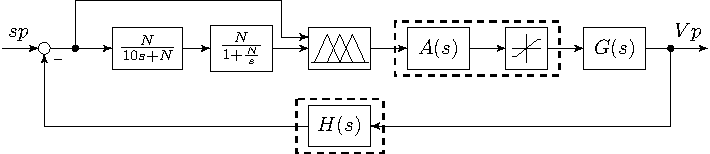
\includegraphics[width=\textwidth]{pdDifuso.pdf}
        \caption[Esquema de control implementado: PD difuso]{\textbf{Esquema de control implementado: PD difuso}. Fuente: Elaboración propia.} 
        \label{fig:pdDifuso}
    \end{figure}
    
    \vfill

    \begin{figure}[htb]
        \centering
        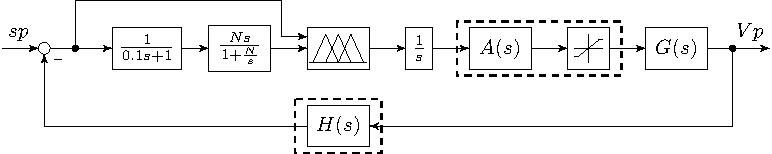
\includegraphics[width=\textwidth]{piDifuso.pdf}
        \caption[Esquema de control implementado: PI difuso]{\textbf{Esquema de control implementado: PI difuso}. Fuente: Elaboración propia.} 
        \label{fig:piDifuso}
    \end{figure}

    \vfill

    \begin{figure}[htb]
        \centering
        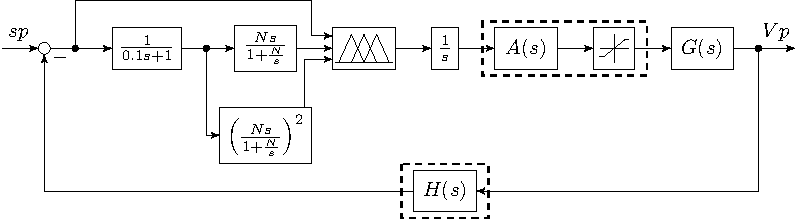
\includegraphics[width=\textwidth]{pidDifuso.pdf}
        \caption[Esquema de control implementado: PID difuso]{\textbf{Esquema de control implementado: PID difuso}. Fuente: Elaboración propia.} 
        \label{fig:pidDifuso}
    \end{figure}
    
    \vfill

    \pagebreak
    
    \vfill

    \begin{figure}[htb]
        \centering
        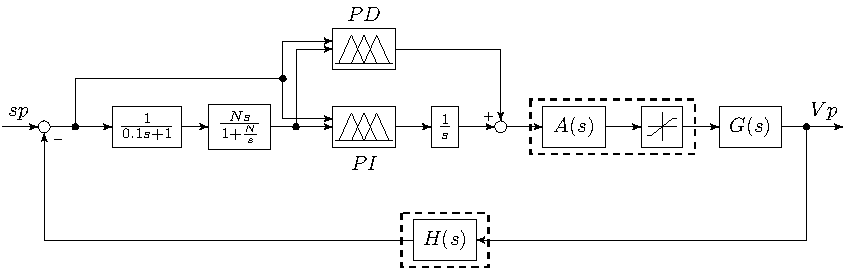
\includegraphics[width=\textwidth]{pipdDifuso.pdf}
        \caption[Esquema de control implementado: PD difuso mas PI difuso]{\textbf{Esquema de control implementado: PD difuso mas PI difuso}. Fuente: Elaboración propia.} 
        \label{fig:pipdDifuso}
    \end{figure}
    
    \vfill

    \begin{figure}[htb]
        \centering
        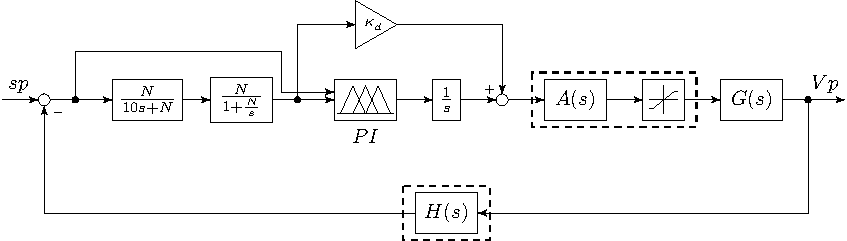
\includegraphics[width=\textwidth]{piplusDDifuso.pdf}
        \caption[Esquema de control implementado: PI difuso más derivada]{\textbf{Esquema de control implementado: PI difuso más derivada}. Fuente: Elaboración propia.} 
        \label{fig:piplusDDifuso}
    \end{figure}
    
    \vfill

    \begin{figure}[htb]
        \centering
        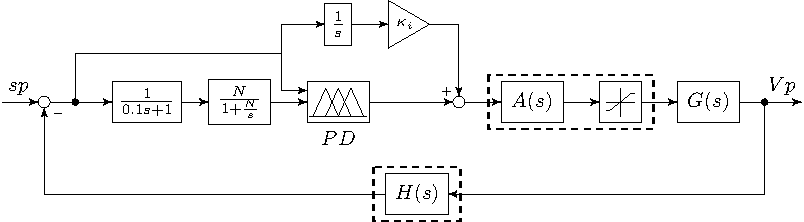
\includegraphics[width=\textwidth]{pdplusIDifuso.pdf}
        \caption[Esquema de control implementado: PD difuso más integrador]{\textbf{Esquema de control implementado: PD difuso más integrador}. Fuente: Elaboración propia.} 
        \label{fig:pdplusIDifuso}
    \end{figure}
    
    \vfill

    \pagebreak
    
    \vfill

    \begin{figure}[htb]
        \centering
        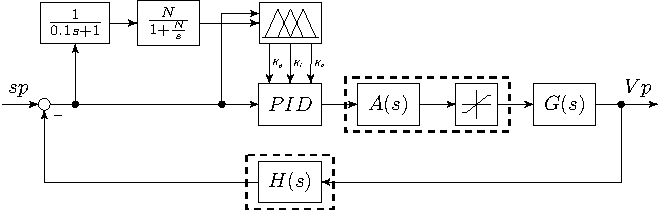
\includegraphics[width=\textwidth]{GainScheduler.pdf}
        \caption[Esquema de control implementado: Programador de ganancias]{\textbf{Esquema de control implementado: Programador de ganancias}. Fuente: Elaboración propia.} 
        \label{fig:GainScheduler}
    \end{figure}
    
    \vfill

    \begin{figure}[htb]
        \centering
        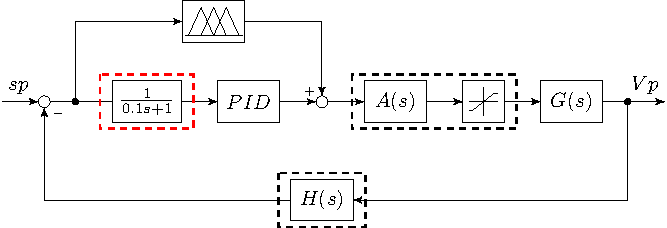
\includegraphics[width=\textwidth]{pidplusDifuso.pdf}
        \caption[Esquema de control implementado: PID clásico más P difuso]{\textbf{Esquema de control implementado: PID clásico mas P difuso}. Fuente: Elaboración propia.} 
        \label{fig:pidplusDifuso}
    \end{figure}
    
    \vfill

\AgregarAnexo{Formato interno para guardar controlador por medio de un archivo .JSON}{anexo:json}
    
    \begin{longlisting}
        \caption[Formato para guardar controlador]{Formato para un controlador con una entrada, una salida y tres reglas. Las reglas son: una simple, una regla con premisa negada y una regla con salida ponderada en 0.25.}
        \label{code:anexoE}				
        \begin{minted}[escapeinside=||,
            mathescape=true,
            autogobble=true,
            fontsize=\scriptsize,
            obeytabs=true,
            tabsize=4,
            baselinestretch=1,
			breaklines]{python}
            [
                [
                    {
                        "nombre": "entrada1",
                        "numeroE": 3,
                        "etiquetas": [
                            {
                                "nombre": "etiqueta1",
                                "mf": "trimf",
                                "definicion": [
                                    -20.0,
                                    -10.0,
                                    0.0
                                ]
                            },
                            {
                                "nombre": "etiqueta2",
                                "mf": "trapmf",
                                "definicion": [
                                    -10.0,
                                    -5.0,
                                    5.0,
                                    10.0
                                ]
                            },
                            {
                                "nombre": "etiqueta3",
                                "mf": "gaussmf",
                                "definicion": [
                                    2.5,
                                    10.0
                                ]
                            }
                        ],
                        "rango": [
                            -10,
                            10
                        ]
                    }
                ],
                [
                    {
                        "nombre": "salida1",
                        "numeroE": 3,
                        "etiquetas": [
                            {
                                "nombre": "etiqueta1",
                                "mf": "gauss2mf",
                                "definicion": [
                                    1.25,
                                    -15.0,
                                    1.25,
                                    -5.0
                                ]
                            },
                            {
                                "nombre": "etiqueta2",
                                "mf": "dsigmf",
                                "definicion": [
                                    1.0,
                                    -5.0,
                                    1.0,
                                    5.0
                                ]
                            },
                            {
                                "nombre": "etiqueta3",
                                "mf": "pimf",
                                "definicion": [
                                    0.0,
                                    5.0,
                                    15.0,
                                    20.0
                                ]
                            }
                        ],
                        "rango": [
                            -10,
                            10
                        ],
                        "metodo": "centroid"
                    }
                ],
                [
                    [
                        [
                            [
                                "etiqueta1",
                                0,
                                false
                            ]
                        ],
                        [
                            [
                                "etiqueta1",
                                0,
                                1.0
                            ]
                        ],
                        true
                    ],
                    [
                        [
                            [
                                "etiqueta2",
                                0,
                                true
                            ]
                        ],
                        [
                            [
                                "etiqueta2",
                                0,
                                1.0
                            ]
                        ],
                        false
                    ],
                    [
                        [
                            [
                                "etiqueta3",
                                0,
                                false
                            ]
                        ],
                        [
                            [
                                "etiqueta3",
                                0,
                                0.24999999999999933
                            ]
                        ],
                        false
                    ]
                ]
            ]
        \end{minted}
    \end{longlisting}

\AgregarAnexo{Códigos para el manejo de archivos FIS}{anexo:codefis}
    
    \begin{longlisting}
        \caption[Extracción de datos del archivo FIS - YAPFLM]{Extracción de datos del archivo FIS - YAPFLM.}
        \label{code:anexoF1}				
        \begin{minted}[escapeinside=||,
            mathescape=true,
            autogobble=true,
            fontsize=\scriptsize,
            obeytabs=true,
            tabsize=4,
            baselinestretch=1,
			breaklines]{python}
            class FISParser:
                """
                [Clase para cargar y exportar archivos .fis, para cargar los archivos FIS las funciones get_system, get_vars,
                get_var y get_rules fueron tomadas de yapflm: 
                
                Yet Another Python Fuzzy Logic Module: https://github.com/sputnick1124/yapflm 
                
                para obtener los datos necesarias del .fis, de allí, se aplica la función fis_to_json para completar el 
                parsin.
                
                En el caso de la exportación, se realiza utilizando la función json_to_fis]
                """

                def __init__(self, file, InputList=None, OutputList=None, RuleEtiquetas=None):
                    """
                    [Constructor de la clase, inicializa las variables a utilizar y selecciona entre cargar el fis o
                    exportarlo dependiendo de las variables con las que se cree el objeto]
                    
                    :param file: [Dirección del archivo a cargar o exportar]
                    :type file: [str]
                    :param inputlist: [Lista de variables de entrada], defaults to None
                    :type inputlist: [list], optional
                    :param OutputList: [Lista de variables de entrada], defaults to None
                    :type OutputList: [list], optional
                    :param RuleEtiquetas: [Lista con la información necesaria para crear las reglas], defaults to None
                    :type RuleEtiquetas: [list], optional
                    """

                    # Cargar archivo .fis
                    if InputList is None and OutputList is None and RuleEtiquetas is None:
                        with open(file, 'r') as infis:
                            self.rawlines = infis.readlines()
                        self.systemList = 0
                        self.InputList = []
                        self.OutputList = []
                        self.RuleList = []
                        self.get_system()
                        self.get_vars()
                        self.get_rules()
                    else:
                        # Exportar archivo .fis
                        self.file = file
                        self.InputList = InputList
                        self.OutputList = OutputList
                        self.RuleEtiquetas = RuleEtiquetas
                        self.json_to_fis()

                def get_system(self):
                    """ [Funcion tomada de yapflm (Yet Another Python Fuzzy Logic Module)] """

                    end_sysblock = self.rawlines.index('\n')
                    systemblock = self.rawlines[1:end_sysblock]
                    fisargs = map(lambda x: parse('{arg}={val}', x), systemblock)
                    fissys = {f['arg'].lower(): f['val'].strip("'") for f in fisargs}
                    self.numinputs = int(fissys['numinputs'])
                    self.numoutputs = int(fissys['numoutputs'])
                    self.numrules = int(fissys['numrules'])
                    self.start_varblocks = end_sysblock + 1
                    self.systemList = fissys

                def get_var(self, vartype, varnum, start_line, end_line):
                    """ [Funcion tomada de yapflm (Yet Another Python Fuzzy Logic Module)] """

                    varblock = self.rawlines[start_line:end_line]
                    fisargs = map(lambda x: parse('{arg}={val}', x), varblock)
                    fisvar = {f['arg'].lower(): f['val'].strip("'") for f in fisargs}

                    if 'input' in vartype:
                        self.InputList.append(fisvar)
                    elif 'output' in vartype:
                        self.OutputList.append(fisvar)

                def get_vars(self):
                    """ [Función tomada de yapflm (Yet Another Python Fuzzy Logic Module)] """

                    start_ruleblock = self.rawlines.index('[Rules]\n')
                    var_lines = []
                    var_types = []
                    flag = 0
                    for i, line in enumerate(self.rawlines[self.start_varblocks - 1:start_ruleblock]):
                        if flag:
                            flag = 0
                            vt = parse('[{type}{num:d}]', line)
                            var_types.append((vt['type'].lower(), vt['num']))
                        if line == '\n':
                            var_lines.append(i + self.start_varblocks - 1)
                            flag = 1
                    for i, l in enumerate(var_lines[:-1]):
                        if 'input' in var_types[i][0]:
                            self.get_var('input', var_types[i][1] - 1, l + 2, var_lines[i + 1])
                        elif 'output' in var_types[i][0]:
                            self.get_var('output', var_types[i][1] - 1, l + 2, var_lines[i + 1])

                def get_rules(self):
                    """ [Función tomada de yapflm (Yet Another Python Fuzzy Logic Module)] """

                    start_ruleblock = self.rawlines.index('[Rules]\n')
                    ruleblock = self.rawlines[start_ruleblock + 1:]
                    antecedents = (('{a%d:d} ' * self.numinputs) %
                                tuple(range(self.numinputs))).strip()
                    consequents = ('{c%d:d} ' * self.numoutputs) % tuple(range(self.numoutputs))
                    p = antecedents + ', ' + consequents + '({w:d}) : {c:d}'
                    for rule in ruleblock:
                        try:
                            p = antecedents + ', ' + consequents + '({w:d}) : {c:d}'
                            rp = parse(p, rule)
                            r = []
                            for inp in range(self.numinputs):
                                rpar = rp['a%d' % inp]
                                rval = rpar if rpar != 0 else None
                                r.append(rval)
                            for outp in range(self.numoutputs):
                                rpar = rp['c%d' % outp]
                                rval = rpar if rpar != 0 else None
                                r.append(rval)
                            r += [rp['w'], rp['c'] - 1]
                            self.RuleList.append(r)
                        except:
                            p = antecedents + ', ' + consequents + '({w:f}) : {c:d}'
                            rp = parse(p, rule)
                            r = []
                            for inp in range(self.numinputs):
                                rpar = rp['a%d' % inp]
                                rval = rpar if rpar != 0 else None
                                r.append(rval)
                            for outp in range(self.numoutputs):
                                rpar = rp['c%d' % outp]
                                rval = rpar if rpar != 0 else None
                                r.append(rval)
                            r += [rp['w'], rp['c'] - 1]
                            self.RuleList.append(r)
        \end{minted}
    \end{longlisting}

    \begin{longlisting}
        \caption[Procesado de los datos del FIS]{Procesado de los datos del FIS, esta función pertenece a la clase FISParser.}
        \label{code:anexoF2}				
        \begin{minted}[escapeinside=||,
            mathescape=true,
            autogobble=true,
            fontsize=\scriptsize,
            obeytabs=true,
            tabsize=4,
            baselinestretch=1,
            breaklines]{python}
            def fis_to_json(self):
                """ [Función para completar la creación del controlador a partir de un archivo .fis] """

                # Datos del controlador
                ni = int(self.systemList['numinputs'])
                no = int(self.systemList['numoutputs'])
                nr = int(self.systemList['numrules'])

                InputList = [0] * ni
                OutputList = [0] * no
                RuleEtiquetas = []

                # Creación de las variables de entrada
                for i in range(ni):
                    InputList[i] = {
                        "nombre":
                            self.InputList[i]['name'],
                        "numeroE":
                            int(self.InputList[i]['nummfs']),
                        "etiquetas": [0] * int(self.InputList[i]['nummfs']),
                        "rango":
                            ast.literal_eval(
                                re.sub("\s+", ",", self.InputList[i]['range'].strip()))
                    }

                    for ne in range(int(self.InputList[i]['nummfs'])):
                        temp_etiqueta = self.InputList[0]['mf' + str(ne + 1)].replace(
                            "'", '').split(':')
                        temp2 = temp_etiqueta[1].split(',')
                        InputList[i]['etiquetas'][ne] = {
                            "nombre": temp_etiqueta[0],
                            "mf": temp2[0],
                            "definicion": ast.literal_eval(re.sub("\s+", ",", temp2[1].strip()))
                        }

                # Creación de las variables de salida
                for i in range(no):
                    OutputList[i] = {
                        "nombre":
                            self.OutputList[i]['name'],
                        "numeroE":
                            int(self.OutputList[i]['nummfs']),
                        "etiquetas": [0] * int(self.OutputList[i]['nummfs']),
                        "rango":
                            ast.literal_eval(
                                re.sub("\s+", ",", self.OutputList[i]['range'].strip())),
                        "metodo":
                            self.systemList['defuzzmethod']
                    }

                    for ne in range(int(self.OutputList[i]['nummfs'])):
                        temp_etiqueta = self.OutputList[i]['mf' + str(ne + 1)].replace(
                            "'", '').split(':')
                        temp2 = temp_etiqueta[1].split(',')
                        OutputList[i]['etiquetas'][ne] = {
                            "nombre": temp_etiqueta[0],
                            "mf": temp2[0],
                            "definicion": ast.literal_eval(re.sub("\s+", ",", temp2[1].strip()))
                        }

                # Creación de las reglas
                for numeror, i in enumerate(self.RuleList):
                    ril = []
                    rol = []

                    for j in range(ni):
                        if i[j] is not None:
                            nombre = InputList[j]['etiquetas'][abs(i[j]) - 1]['nombre']
                            numero = j
                            negacion = False if i[j] > 0 else True
                            ril.append([nombre, numero, negacion])

                    for j in range(ni, no + ni):
                        if i[j] is not None:
                            if i[j] < 0:
                                raise TypeError('No se permiten salidas negadas')
                            nombre = OutputList[j - ni]['etiquetas'][abs(i[j]) - 1]['nombre']
                            numero = j - ni
                            peso = float(i[no + ni])
                            rol.append([nombre, numero, peso])

                    and_condition = True if i[ni + no + 1] == 0 else False
                    RuleEtiquetas.append(copy.deepcopy([ril, rol, and_condition]))

                return copy.deepcopy(InputList), copy.deepcopy(OutputList), copy.deepcopy(RuleEtiquetas)
        \end{minted}
    \end{longlisting}

    \pagebreak

    \begin{longlisting}
        \caption[Exportar archivos FIS]{Exportar archivos FIS, esta función pertenece a la clase FISParser.}
        \label{code:anexoF3}				
        \begin{minted}[escapeinside=||,
            mathescape=true,
            autogobble=true,
            fontsize=\scriptsize,
            obeytabs=true,
            tabsize=4,
            baselinestretch=1,
            breaklines=true,
            breakbytokenanywhere=true]{python}
            def json_to_fis(self):
                """ [Función para exportar el controlador en formato .fis] """

                # Datos del controlador
                ni = len(self.InputList)
                no = len(self.OutputList)
                nr = len(self.RuleEtiquetas)

                with open(self.file, 'w') as f:

                    # Información general del controlador
                    f.write(f"[System]\n")
                    f.write(f"Name='{self.file.split('/')[-1].split('.')[0]}'\n")
                    f.write(f"Type='mamdani'\n")
                    f.write(f"Version=2.0\n")
                    f.write(f"NumInputs={ni}\n")
                    f.write(f"NumOutputs={no}\n")
                    f.write(f"NumRules={nr}\n")
                    f.write(f"AndMethod='min'\n")
                    f.write(f"OrMethod='max'\n")
                    f.write(f"ImpMethod='min'\n")
                    f.write(f"AggMethod='max'\n")
                    f.write(f"DefuzzMethod='{self.OutputList[0]['metodo']}'\n")
                    f.write(f"\n")

                    # Parsin de las entradas del controlador
                    for i in range(ni):
                        f.write(f"[Input" + str(i + 1) + "]\n")
                        f.write(f"Name='{self.InputList[i]['nombre']}'\n")
                        string_temp = re.sub('\s+', '',
                                            str(self.InputList[i]['rango'])).replace(',', ' ')
                        f.write(f"Range={string_temp}\n")
                        f.write(f"NumMFs={self.InputList[i]['numeroE']}\n")

                        for ne in range(self.InputList[i]['numeroE']):
                            string_temp = re.sub(
                                '\s+', '',
                                str(self.InputList[i]['etiquetas'][ne]['definicion'])).replace(
                                    ',', ' ')
                            f.write(
                                f"MF{ne+1}='{self.InputList[i]['etiquetas'][ne]['nombre']}"
                                f"':'{self.InputList[i]['etiquetas'][ne]['mf']}',{string_temp}\n"
                            )

                        f.write(f"\n")

                    # Parsin de las salidas del controlador
                    for i in range(no):
                        f.write(f"[Output" + str(i + 1) + "]\n")
                        f.write(f"Name='{self.OutputList[i]['nombre']}'\n")
                        string_temp = re.sub('\s+', '',
                                            str(self.OutputList[i]['rango'])).replace(',', ' ')
                        f.write(f"Range={string_temp}\n")
                        f.write(f"NumMFs={self.OutputList[i]['numeroE']}\n")

                        for ne in range(self.OutputList[i]['numeroE']):
                            string_temp = re.sub(
                                '\s+', '',
                                str(self.OutputList[i]['etiquetas'][ne]['definicion'])).replace(
                                    ',', ' ')
                            f.write(
                                f"MF{ne+1}='{self.OutputList[i]['etiquetas'][ne]['nombre']}"
                                f"':'{self.OutputList[i]['etiquetas'][ne]['mf']}',{string_temp}\n"
                            )

                        f.write(f"\n")

                    # Parsin de las reglas del controlador
                    rules_no_format = []
                    for i, rule in enumerate(self.RuleEtiquetas):

                        inner_rules = []

                        # set de entradas
                        for nir in range(ni):
                            for inputrule in rule[0]:
                                if nir == inputrule[1]:
                                    if not inputrule[2]:
                                        for ner, etiqueta in enumerate(self.InputList[nir]['etiquetas']):
                                            if etiqueta['nombre'] == inputrule[0]:
                                                inner_rules.append(ner + 1)
                                                break
                                    else:
                                        for ner, etiqueta in enumerate(self.InputList[nir]['etiquetas']):
                                            if etiqueta['nombre'] == inputrule[0]:
                                                inner_rules.append(-ner - 1)
                                                break

                                    break
                                else:
                                    continue
                            else:
                                inner_rules.append(0)
                                break

                        # set de salidas
                        for nor in range(no):
                            for outputtrule in rule[1]:
                                if nor == outputtrule[1]:
                                    for ner, etiqueta in enumerate(self.OutputList[nor]['etiquetas']):
                                        if etiqueta['nombre'] == outputtrule[0]:
                                            inner_rules.append(ner + 1)
                                            break
                                    break
                                else:
                                    continue
                            else:
                                inner_rules.append(0)

                        inner_rules.append(rule[1][0][2])

                        if rule[2]:
                            inner_rules.append(1)
                        else:
                            inner_rules.append(2)

                        rules_no_format.append(copy.deepcopy(inner_rules))

                    f.write(f"[Rules]\n")

                    # Escribiendo las reglas en el archivo
                    for i in range(nr):
                        rule_str = ""
                        for j in range(ni):
                            if not j == ni - 1:
                                rule_str += str(rules_no_format[i][j]) + " "
                            else:
                                rule_str += str(rules_no_format[i][j])
                        rule_str += ", "
                        for j in range(ni, ni + no):
                            rule_str += str(rules_no_format[i][j]) + " "
                        rule_str += f"({str(rules_no_format[i][ni+no])})" + " "
                        rule_str += f": {str(rules_no_format[i][ni+no+1])}\n"
                        f.write(rule_str)
                return
        \end{minted}
    \end{longlisting}

\AgregarAnexo{Tablas de Butcher para los métodos de Runge-Kutta}{anexo:butcher}

    \vspace{-10pt}

    \section*{Métodos explícitos} 

    \vspace{-20pt}

    \noindent\begin{minipage}[t]{.5\linewidth}
        \subsection{Runge-Kutta de orden 2}
            \begin{equation}\label{eq:rk2}
                \renewcommand\arraystretch{1.2}
                \begin{array}{c|cc}
                0\\
                1/2 & 1/2\\
                \hline
                & 0 & 1
                \end{array}
            \end{equation}
    \end{minipage}%
    \begin{minipage}[t]{.5\linewidth}
        \subsection{Runge-Kutta de orden 3}
            \begin{equation}\label{eq:rk3}
                \renewcommand\arraystretch{1.2}
                \begin{array}{c|ccc}
                0\\
                1/2 & 1/2\\
                1 & -1 & 2\\
                \hline
                & 1/6& 2/3 & 1/6
                \end{array}
            \end{equation}
    \end{minipage}
    
    \vfill
    
    \noindent\begin{minipage}[t]{.5\linewidth}
        \subsection{Heun de orden 3}
            \begin{equation}\label{eq:heun3}
                \renewcommand\arraystretch{1.2}
                \begin{array}{c|ccc}
                0\\
                1/3 & 1/3\\
                2/3 & 0 & 2/3\\
                \hline
                & 1/4 & 0 & 3/4
                \end{array}
            \end{equation}
    \end{minipage}%
    \begin{minipage}[t]{.5\linewidth}
        \subsection{Ralston de orden 3}
            \begin{equation}\label{eq:ralston3}
                \renewcommand\arraystretch{1.2}
                \begin{array}{c|ccc}
                0\\
                1/2 & 1/2\\
                3/4 & 0 & 3/4\\
                \hline
                & 2/9 & 1/3 & 4/9
                \end{array}
            \end{equation}
    \end{minipage}

    \vfill

    \noindent\begin{minipage}[t]{.5\linewidth}
        \subsection{SSPRK de orden 3}
            \begin{equation}\label{eq:ssprk3}
                \renewcommand\arraystretch{1.2}
                \begin{array}{c|ccc}
                0\\
                1 & 1\\
                1/2 & 1/4 & 1/4\\
                \hline
                & 1/6 & 1/6 & 2/3
                \end{array}
            \end{equation}
    \end{minipage}%
    \begin{minipage}[t]{.5\linewidth}
        \subsection{Runge-Kutta de orden 4}
            \begin{equation}\label{eq:rk4}
                \renewcommand\arraystretch{1.2}
                \begin{array}{c|cccc}
                0\\
                1/2 & 1/2\\
                1/2 & 0 & 1/2\\
                1 & 0 & 0& 1\\
                \hline
                & 1/6 & 1/3 & 1/3 & 1/6
                \end{array}
            \end{equation}
    \end{minipage}
    
    \vfill
    
    \pagebreak

    \subsection{Runge-Kutta 3/8 de orden 4}
    \vspace{-10pt}
        \begin{equation}\label{eq:rk38}
            \renewcommand\arraystretch{1.2}
            \begin{array}{c|cccc}
            0\\
            1/3 & 1/3\\
            2/3 & -1/3 & 1\\
            1 & 1 & -1& 1\\
            \hline
            & 1/8 & 3/8 & 3/8 & 1/8
            \end{array}
        \end{equation}
    
    \subsection{Ralston con mínimo error de truncamiento de orden 4}
    \vspace{-10pt}
        \begin{equation}\label{eq:ralston4}
            \renewcommand\arraystretch{1.2}
            \begin{array}{c|cccc}
            0\\
            0.4 & 0.4\\
            0.45573725 & 0.29697761 & 0.15875964\\
            1 & 0.21810040 & -3.05096516 & 3.83286476\\
            \hline
            & 0.17476028 & -0.55148066 & 1.20553560 & 0.17118478
            \end{array}
        \end{equation}

    \subsection{Runge-Kutta de orden 5}
    \vspace{-10pt}
        \begin{equation}\label{eq:rk5}
            \renewcommand\arraystretch{1.2}
            \begin{array}{c|cccccc}
            0\\
            1/4 & 1/4\\
            1/4 & 1/8 & 1/8\\
            1/2 & 0 & -1/2 & 1\\
            3/4 & 3/16 & 0 & 0 & 9/16 \\
            1 & -3/7 & 2/7 & 12/7 & -12/7 & 8/7 \\
            \hline
            & 7/90 & 0 & 32/90 & 12/90 & 32/90 & 7/90
            \end{array}
        \end{equation}
    
    \vspace{-10pt}

    \section*{Métodos embebidos}
    
    \vfill
    
    \subsection{Bogacki-Shampine de orden 3(2)}
    \vspace{-10pt}
        \begin{equation}\label{eq:bogasham23}
            \renewcommand\arraystretch{1.2}
            \begin{array}{c|cccc}
            0\\
            1/2 & 1/2\\
            3/4 & 0 & 3/4\\
            1 & 2/9 & 1/3 & 4/9\\
            \hline
            & 2/9 & 1/3 & 4/9 & 0 \\
            \hline
            & 7/24 & 1/4 & 1/3 & 1/8
            \end{array}
        \end{equation}
    
    \vfill
    
    \subsection{Fehlberg  de orden 4(5)}
        \vspace{-10pt}
            \begin{equation}\label{eq:fehlberg45}
                \renewcommand\arraystretch{1.2}
                \begin{array}{c|cccccc}
                0\\
                1/4 & 1/4\\
                3/8 & 3/32 & 9/32\\
                12/13 & 1932/2197 & -7200/2197 & 7296/2197\\
                1 & 439/216 & -8 & 3680/513 & -845/4104\\
                1/2 & -8/27 & 2 & -3544/2565 & 1859/4104 & -11/40\\
                \hline
                & 25/216 & 0 & 1408/2565 & 2197/4104 & -1/5 & 0\\
                \hline
                & 16/135 & 0 & 6656/12825 & 28561/56430 & -9/50 & 2/55
                \end{array}
            \end{equation}
    
    \vfill
    
    \pagebreak

    \subsection{Cash-Karp de orden 4(5)}
    \vspace{-10pt}
        \begin{equation}\label{eq:cashkarp45}
            \arraycolsep=2.2pt
            \renewcommand\arraystretch{1.2}
            \begin{array}{c|cccccc}
            0\\
            1/5 & 1/5\\
            3/10 & 3/40 & 9/40\\
            3/5 & 3/10 & -9/10 & 6/5\\
            1 & -11/54 & 5/2 & -70/27 & 35/27\\
            7/8 & 1631/55296 & 175/512 & 575/13824 & 44275/110592 & 253/4096\\
            \hline
            & 2825/27648 & 0 & 18575/48384 & 13525/55296 & 277/14336 & 1/4\\
            \hline
            & 37/378 & 0 & 250/621 & 125/594 & 0 & 512/1771
            \end{array}
        \end{equation}
    
    
    \vfill

    \subsection{Dormand-Prince de orden 5(4)}
    \vspace{-10pt}
        \begin{equation}\label{eq:dopri54}
            \small
            \arraycolsep=1.65pt
            \renewcommand\arraystretch{1.2}
            \begin{array}{c|ccccccc}
            0\\
            1/5 & 1/5\\
            3/10 & 3/40 & 9/40\\
            4/5 & 44/45 & -56/15 & 32/9\\
            8/9 & 19372/6561 & -25360/2187 & 64448/6561 & -212/729\\
            1 & 9017/3168 & -355/33 & 46732/5247 & 49/176 & -5103/18656\\
            1 & 35/384 & 0 & 500/1113 & 125/192 & -2187/6784 & 11/84\\
            \hline
            & 35/384 & 0 & 500/1113 & 125/192 & -2187/6784 & 11/84\\
            \hline
            & 5179/57600 & 0 & 7571/16695 & 393/640 & -92097/339200 & 187/2100 & 1/40
            \end{array}
        \raisetag{3cm}
        \end{equation}

\AgregarAnexo{Códigos para el tamaño de paso variable}{anexo:stepsize}
    
    \begin{longlisting}
        \caption[Tamaño de paso variable para Runke-Kutta explícitos]{Tamaño de paso variable para Runke-Kutta explícitos.}
        \label{code:explicitos}				
        \begin{minted}[escapeinside=||,
            mathescape=true,
            autogobble=true,
            fontsize=\scriptsize,
            obeytabs=true,
            tabsize=4,
            baselinestretch=1,
            breaklines=true,
            breakanywhere=true]{python}
            def rk_doble_paso_adaptativo(systema,
                                         h_ant,
                                         tiempo,
                                         tbound,
                                         xVectB,
                                         entrada,
                                         metodo,
                                         ordenq,
                                         rtol,
                                         atol,
                                         max_step_increase,
                                         min_step_decrease,
                                         safety_factor):
                
                while True:
                    # Para asegurar el tiempo máximo
                    if tiempo + h_ant >= tbound:
                        h_ant = tbound - tiempo
                        yS, xVectSn = metodo(*systema, xVectB, h_ant, entrada)
                        h_est = h_ant
                    else:
                        # Paso de tamaño regular
                        yB, xVectBn = metodo(*systema, xVectB, h_ant, entrada)

                        # Dos pasos de tamaño medio
                        yS, xVectSn = metodo(*systema, xVectB, h_ant / 2, entrada)
                        yS, xVectSn = metodo(*systema, xVectSn, h_ant / 2, entrada)

                        # Ajuste del tamaño de paso
                        scale = atol + rtol * (np.abs(xVectBn) + np.abs(xVectSn)) / 2
                        delta1 = np.abs(xVectBn - xVectSn)
                        error_norm = norm(delta1 / scale)

                        if error_norm == 0:
                            # Incremento máximo dado el bajo error
                            h_est = h_ant * max_step_increase
                        elif error_norm <= 1:
                            # Incremento normal
                            h_est = h_ant * min(max_step_increase,
                                                max(1, safety_factor * error_norm**(-1 / (ordenq+1))))
                        else:
                            # Decremento normal y se vuelve a calcular la salida
                            h_ant = h_ant * min(
                                1,
                                max(min_step_decrease, safety_factor * error_norm**(-1 / (ordenq+1))))
                            continue
                    break
                return h_ant, h_est, yS, xVectSn
        \end{minted}
    \end{longlisting}

    \pagebreak

    \begin{longlisting}
        \caption[Tamaño de paso variable para Runke-Kutta embebidos]{Tamaño de paso variable para Runke-Kutta embebidos.}
        \label{code:embebidos}				
        \begin{minted}[escapeinside=||,
            mathescape=true,
            autogobble=true,
            fontsize=\scriptsize,
            obeytabs=true,
            tabsize=4,
            baselinestretch=1,
            breaklines=true,
            breakanywhere=true]{python}
            def rk_embebido_adaptativo(systema,
                                       h_ant,
                                       tiempo,
                                       tbound,
                                       xVectr,
                                       entrada,
                                       metodo,
                                       ordenq,
                                       rtol,
                                       atol,
                                       max_step_increase,
                                       min_step_decrease,
                                       safety_factor):
                
                while True:
                    # Para asegurar el tiempo máximo
                    if tiempo + h_ant >= tbound:
                        h_ant = tbound - tiempo
                        yr, xr, xtemp = metodo(*systema, xVectr, h_ant, entrada)
                        h_est = h_ant
                    else:
                        # Método embebido, la integración se continua con yr y xr
                        yr, xr, xtemp = metodo(*systema, xVectr, h_ant, entrada)

                        # Ajuste del tamaño de paso
                        scale = atol + np.maximum(np.abs(xVectr), np.abs(xr)) * rtol
                        delta1 = np.abs(xr - xtemp)
                        error_norm = norm(delta1 / scale)

                        if error_norm == 0:
                            # Incremento máximo dado el bajo error
                            h_est = h_ant * max_step_increase
                        elif error_norm <= 1:
                            # Incremento normal
                            h_est = h_ant * min(max_step_increase,
                                                max(1, safety_factor * error_norm**(-1 / (ordenq+1))))
                        else:
                            # Decremento normal y se vuelve a calcular la salida
                            h_ant = h_ant * min(
                                1,
                                max(min_step_decrease, safety_factor * error_norm**(-1 / (ordenq+1))))
                            continue
                    break
                return h_ant, h_est, yr, xr
        \end{minted}
    \end{longlisting}

    \begin{longlisting}
        \caption[Función para calcular la norma RMS]{Función para calcular la norma RMS, se realizó un pre compilado con numba para aumentar la velocidad de ejecucion.}
        \label{code:normarms}				
        \begin{minted}[escapeinside=||,
            mathescape=true,
            autogobble=true,
            fontsize=\scriptsize,
            obeytabs=true,
            tabsize=4,
            baselinestretch=1,
            breaklines=true,
            breakanywhere=true]{python}
            @cc.export('norm', 'f8(f8[:,::1])')
            def norm(x):
                """ [Función para calcular la norma RMS de un vector. Función tomada de SciPy] """
                return np.linalg.norm(x) / x.size**0.5
        \end{minted}
    \end{longlisting}

\AgregarAnexo{Comparación gráfica para el análisis de sistemas de control}{anexo:CAnalisis}
        
    \begin{figure}[!h]
        \centering
        \begin{subfigure}[t]{0.99\textwidth}
            \centering
            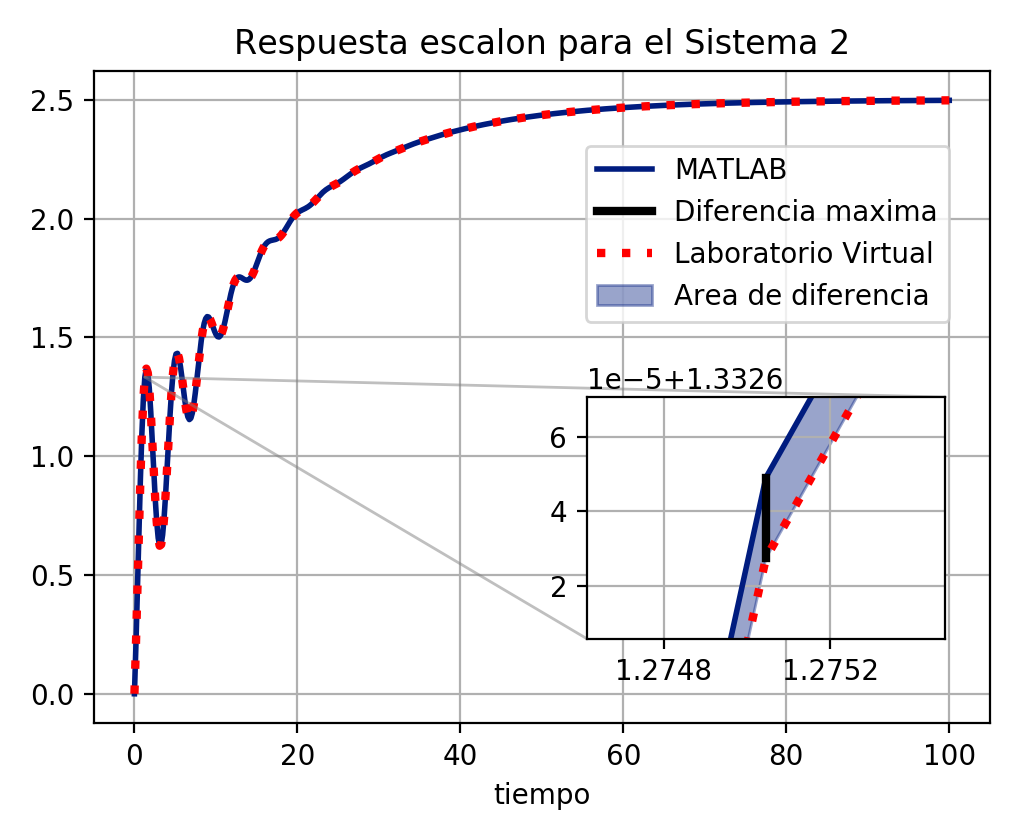
\includegraphics[width=0.43\textwidth,valign=c]{MATLAB/Set2Step.png}
            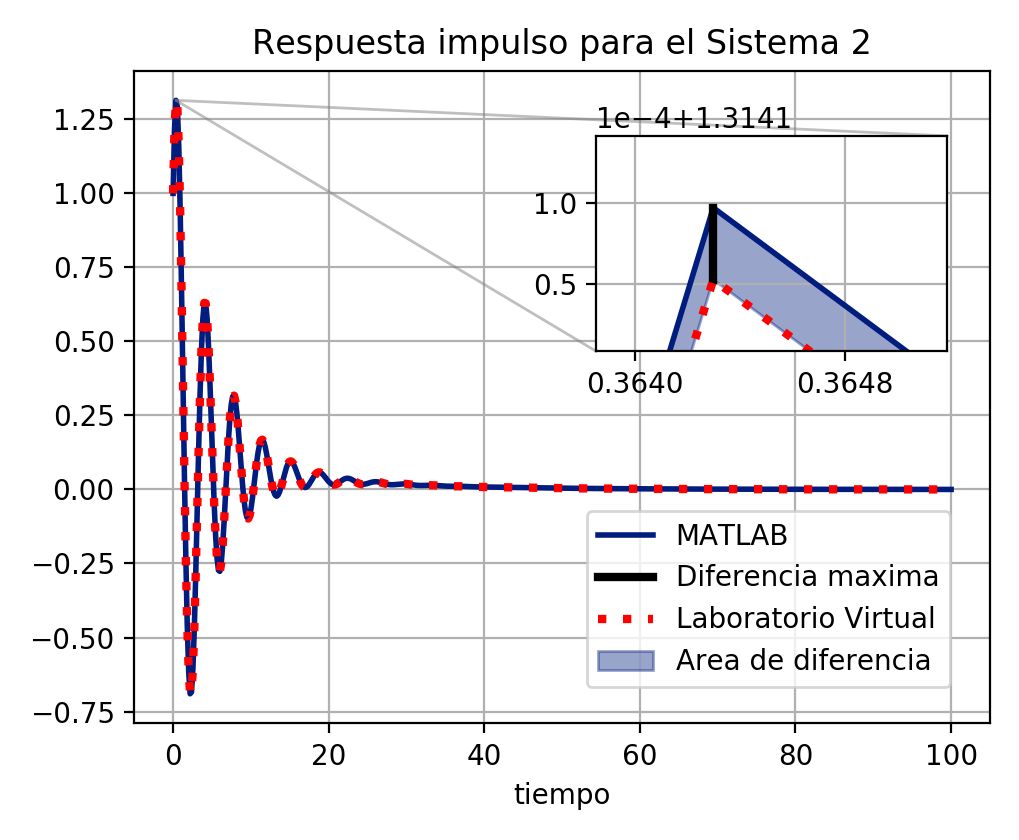
\includegraphics[width=0.43\textwidth,valign=c]{MATLAB/Set2Imp.png}
            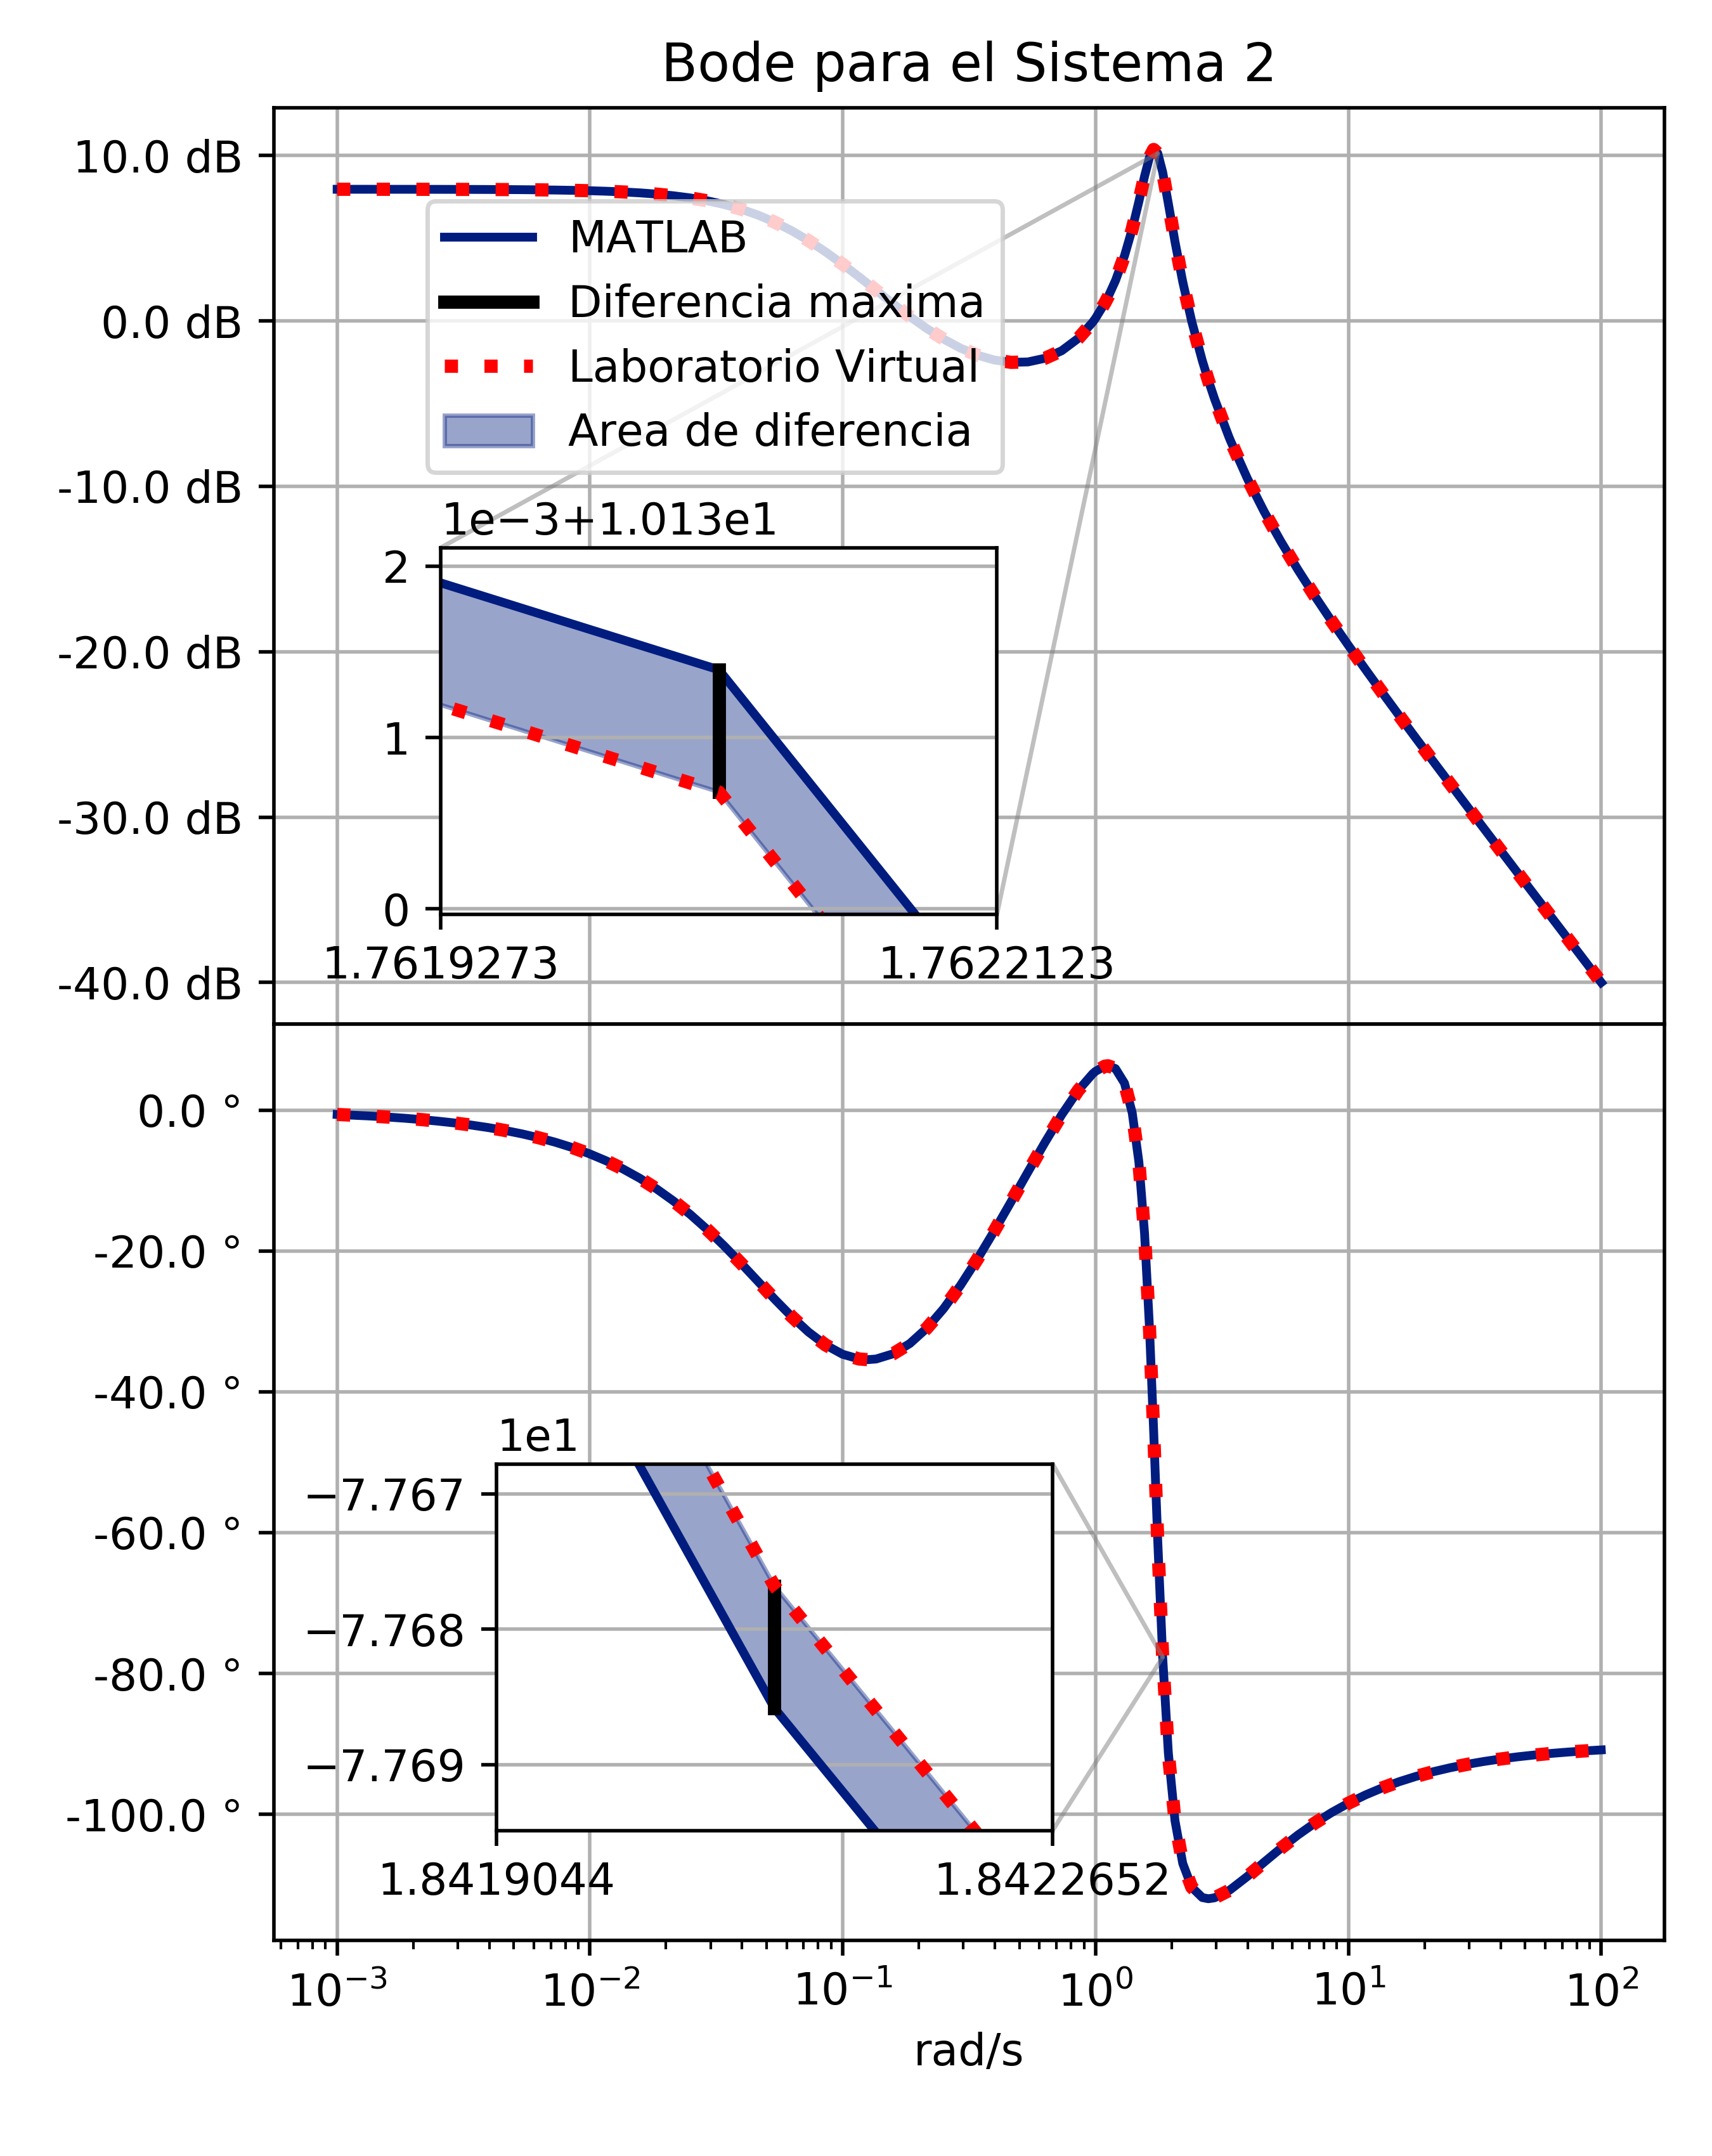
\includegraphics[width=0.43\textwidth,valign=c]{MATLAB/Set2Bode.png}
            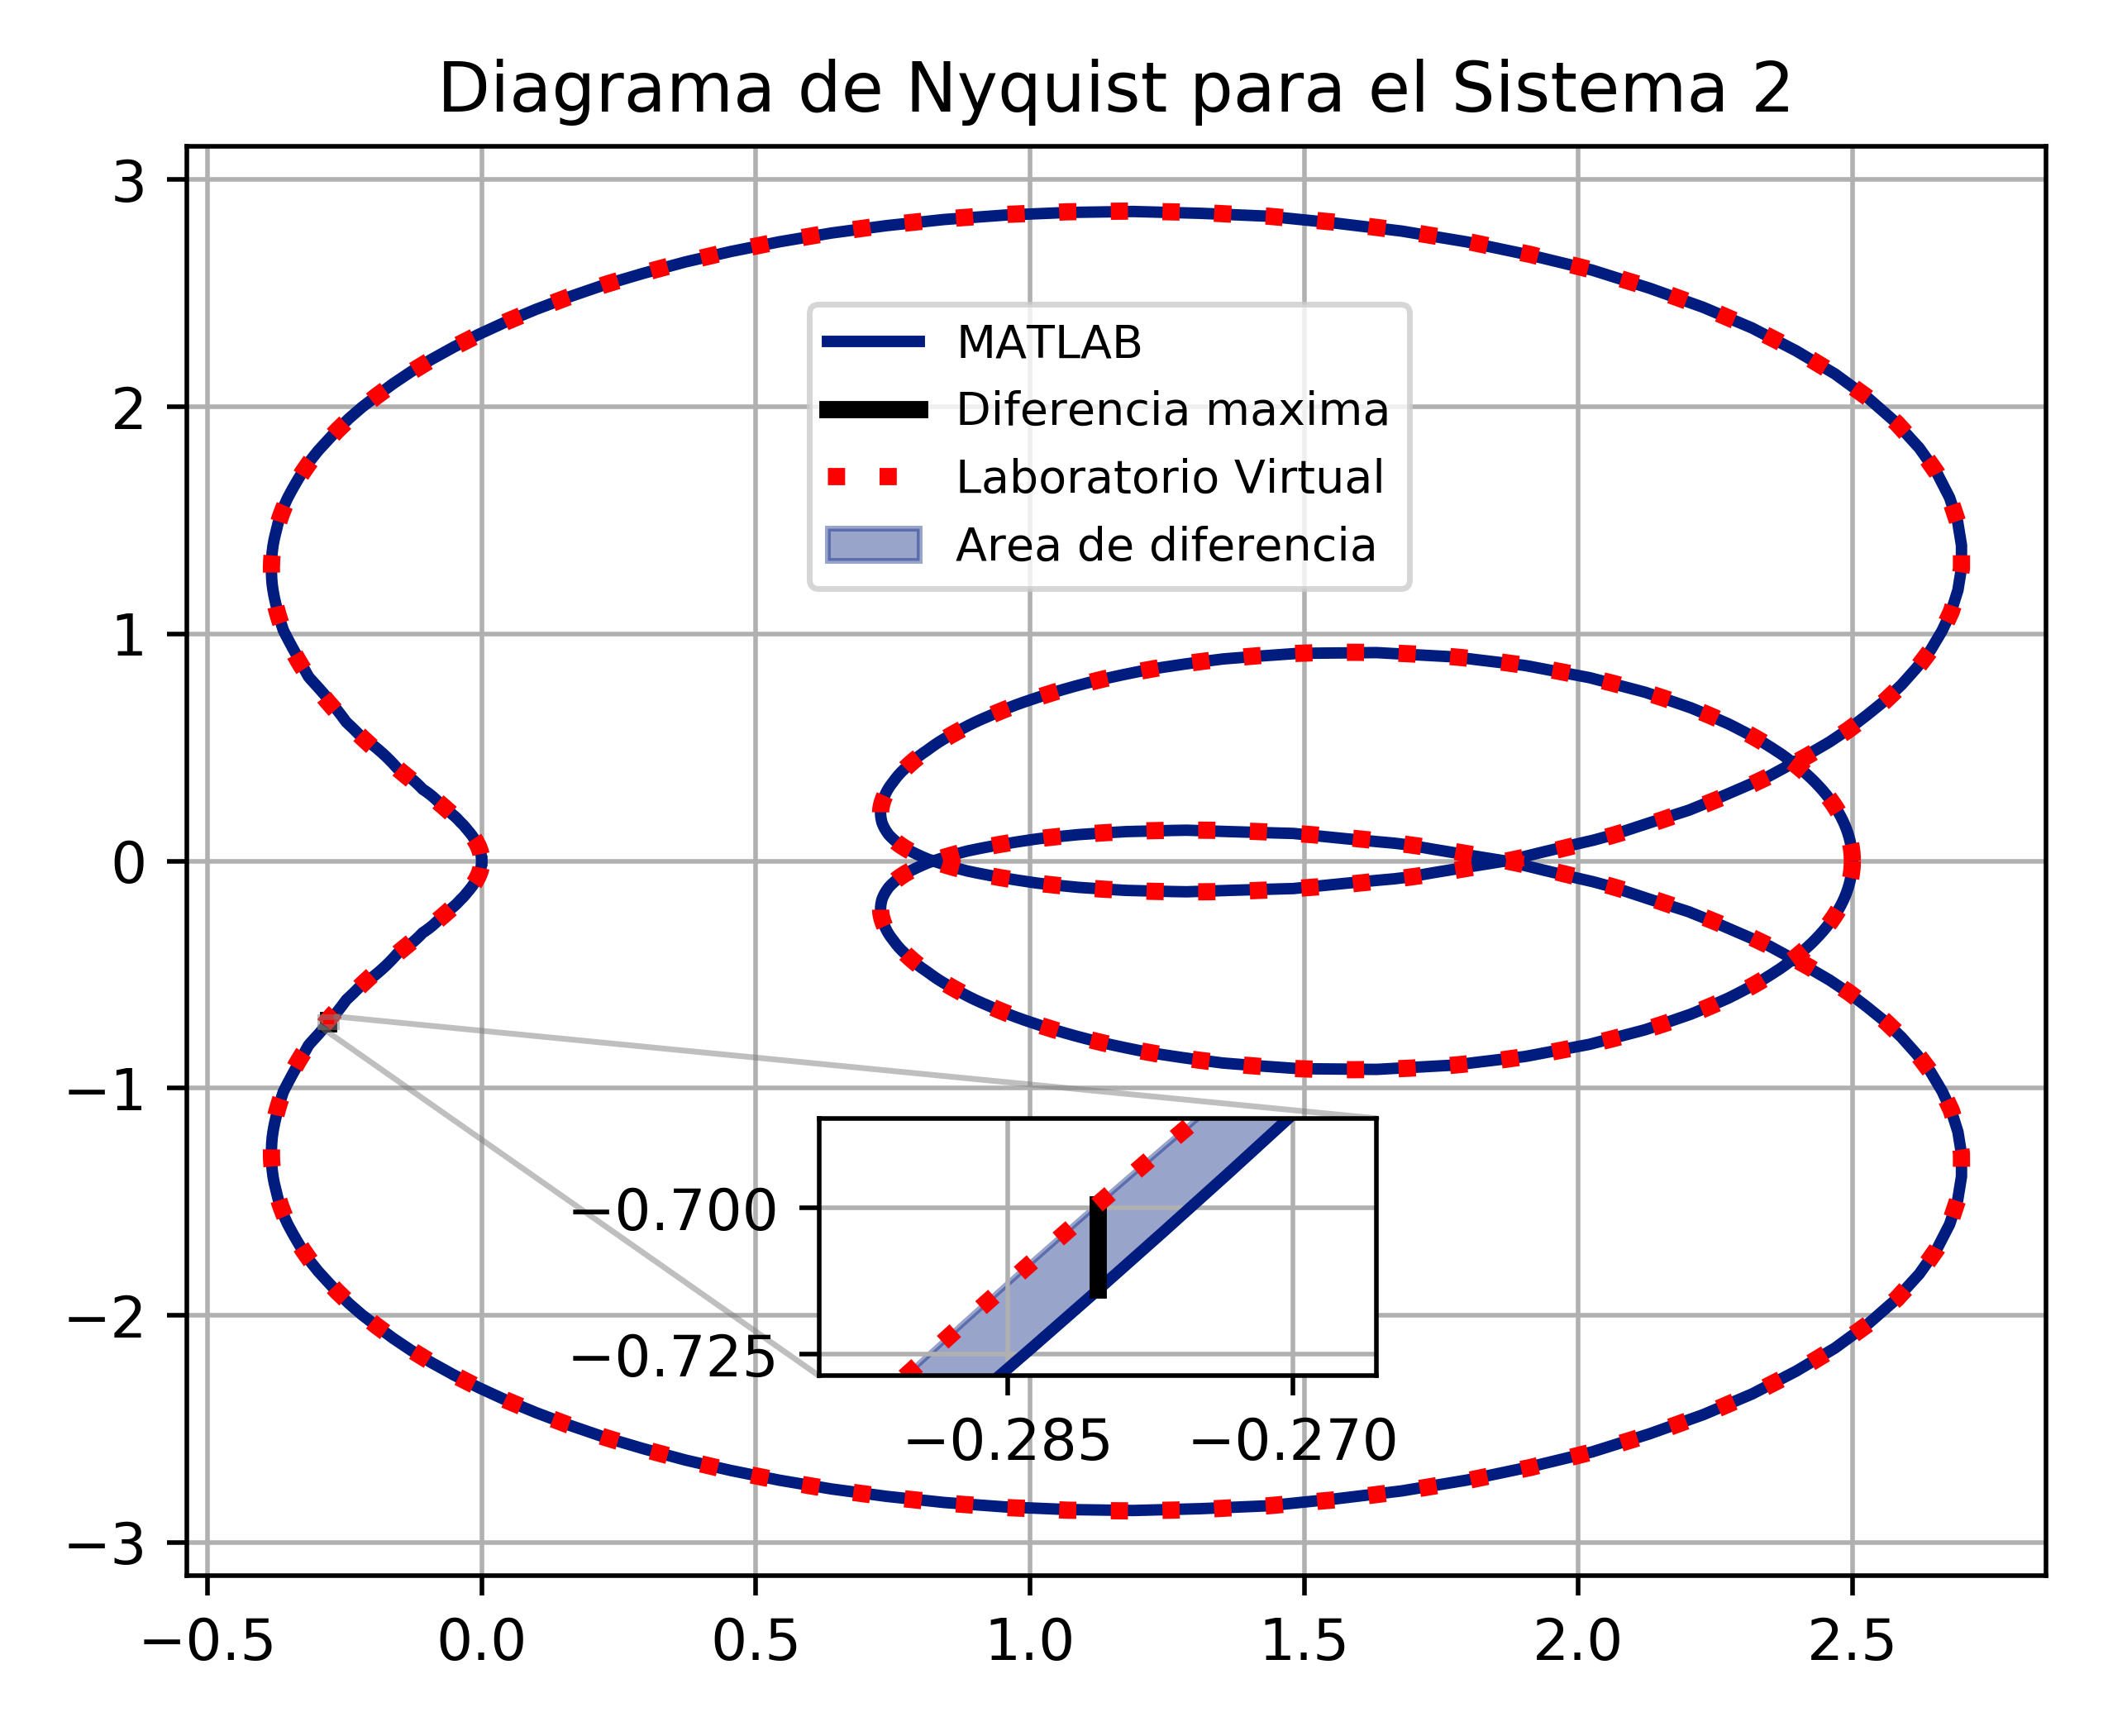
\includegraphics[width=0.43\textwidth,valign=c]{MATLAB/Set2Nyquist.png}
            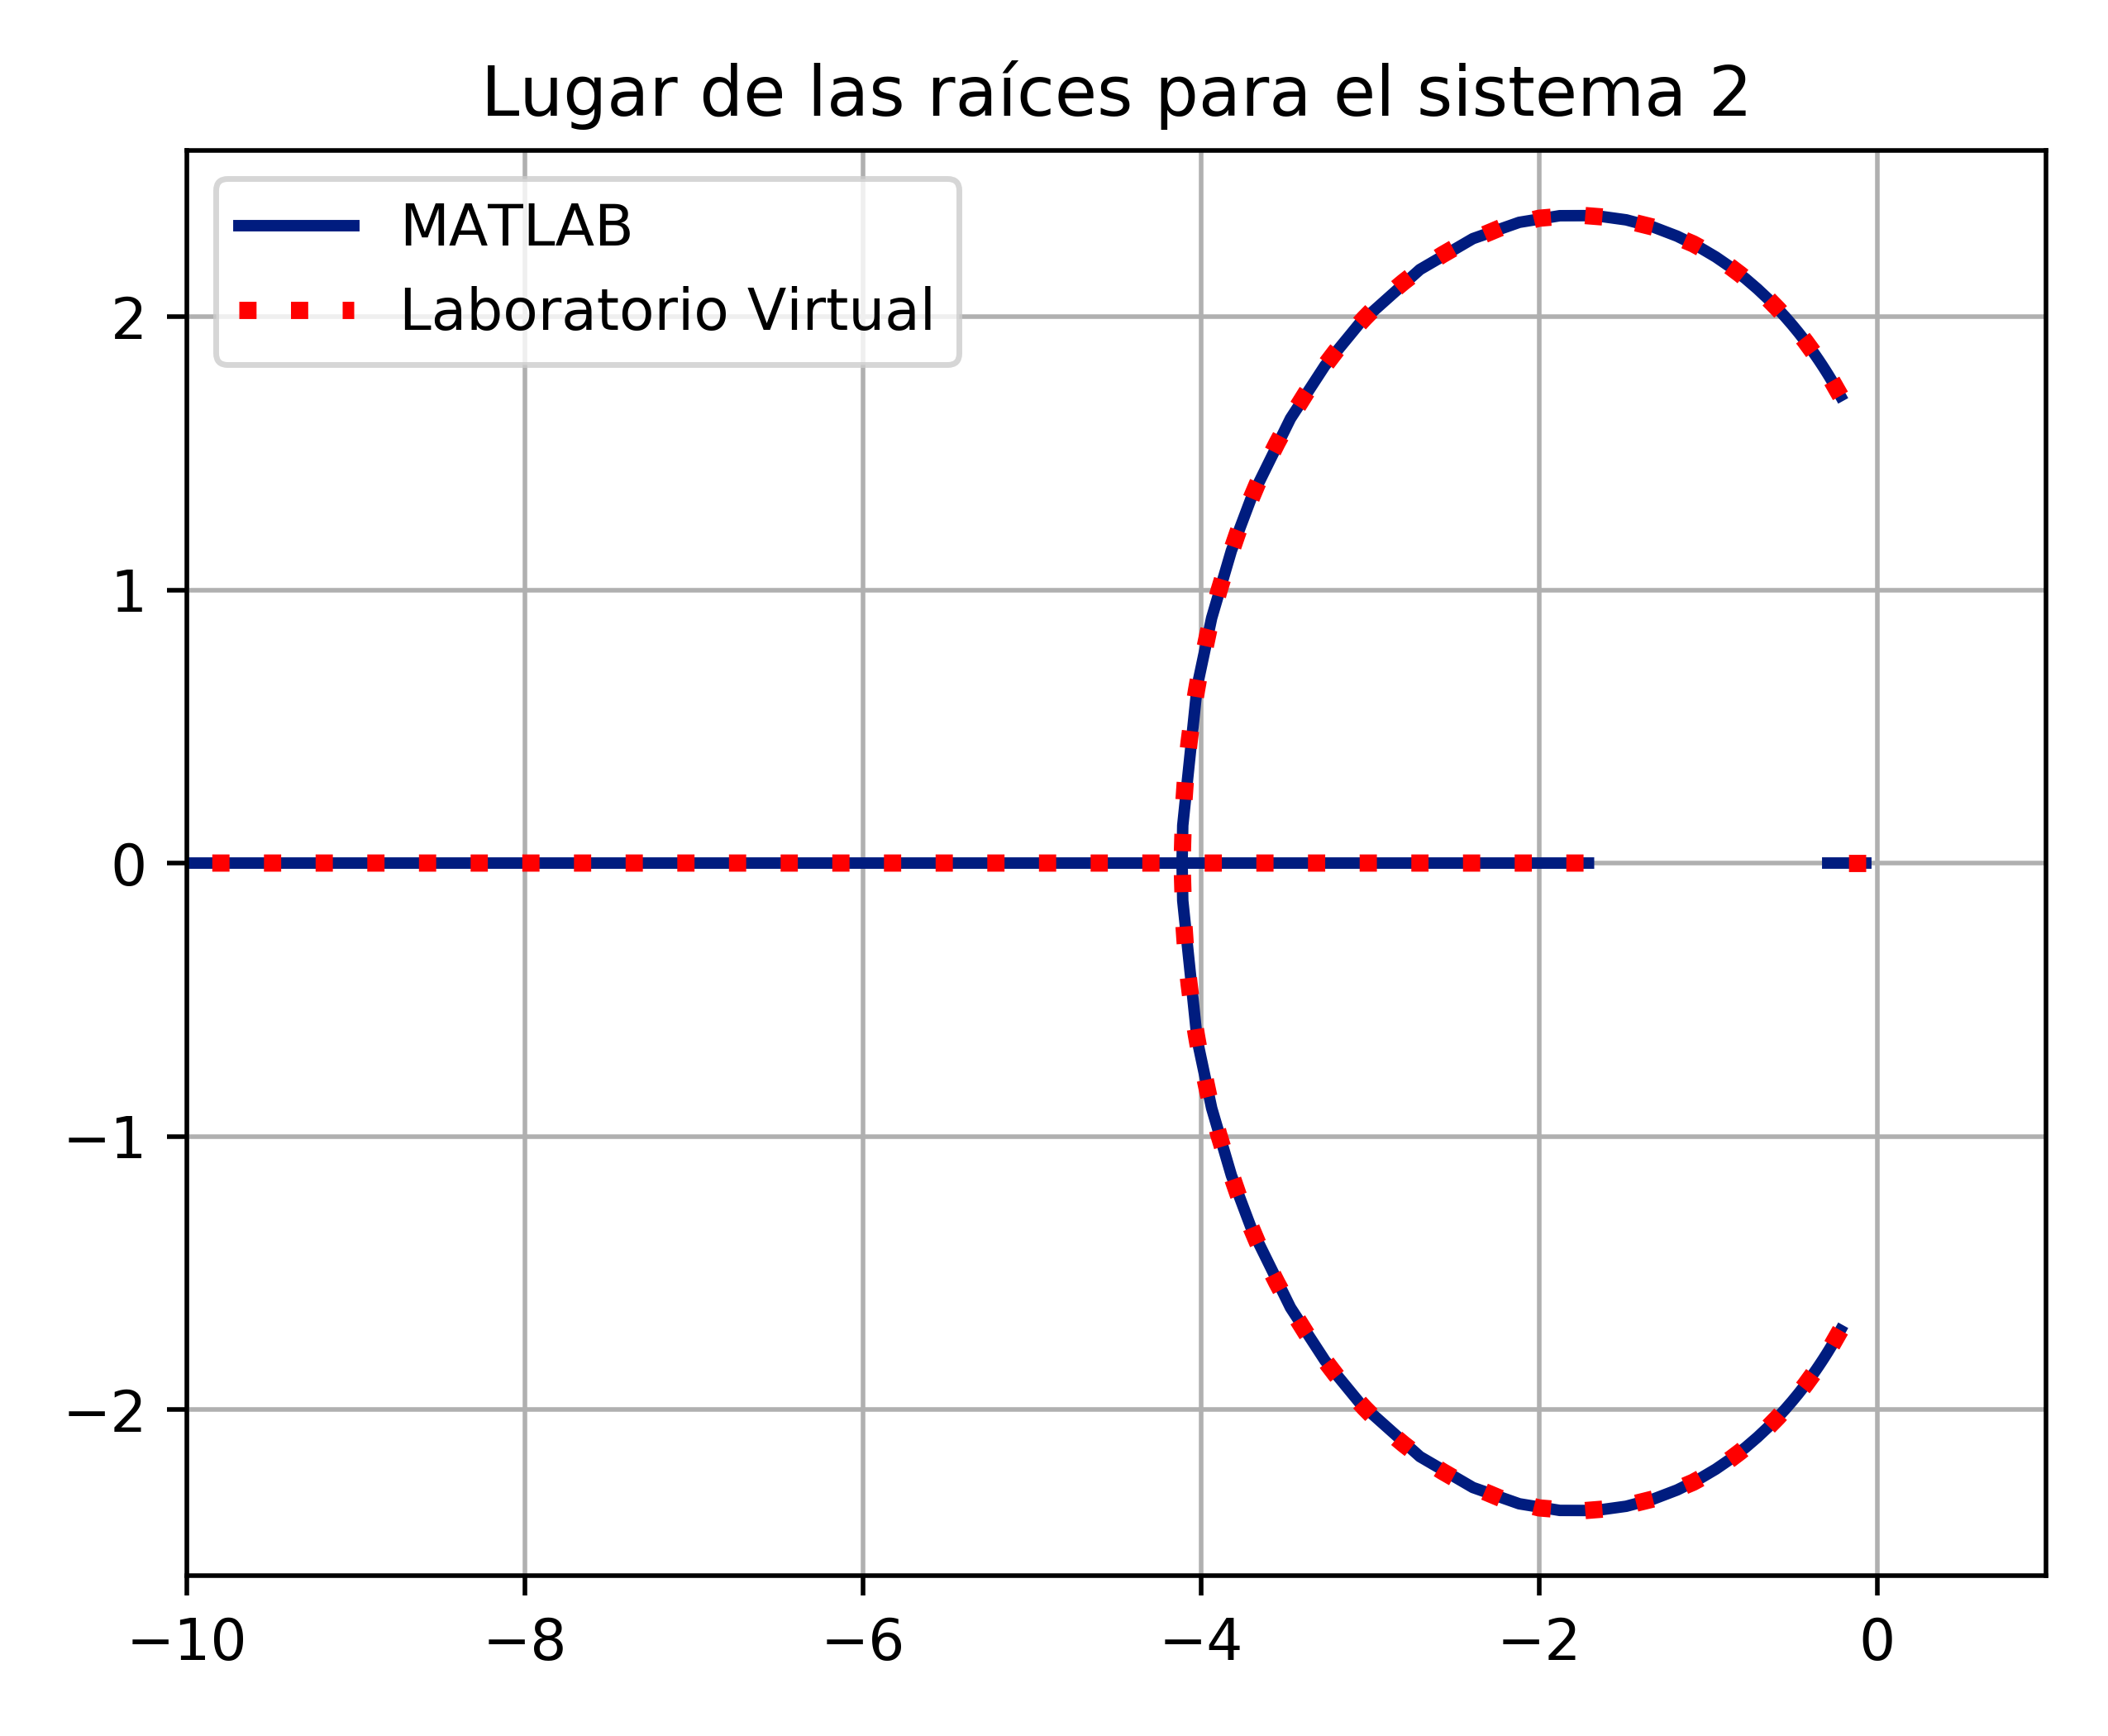
\includegraphics[width=0.43\textwidth,valign=c]{MATLAB/Set2Rlocus.png}
            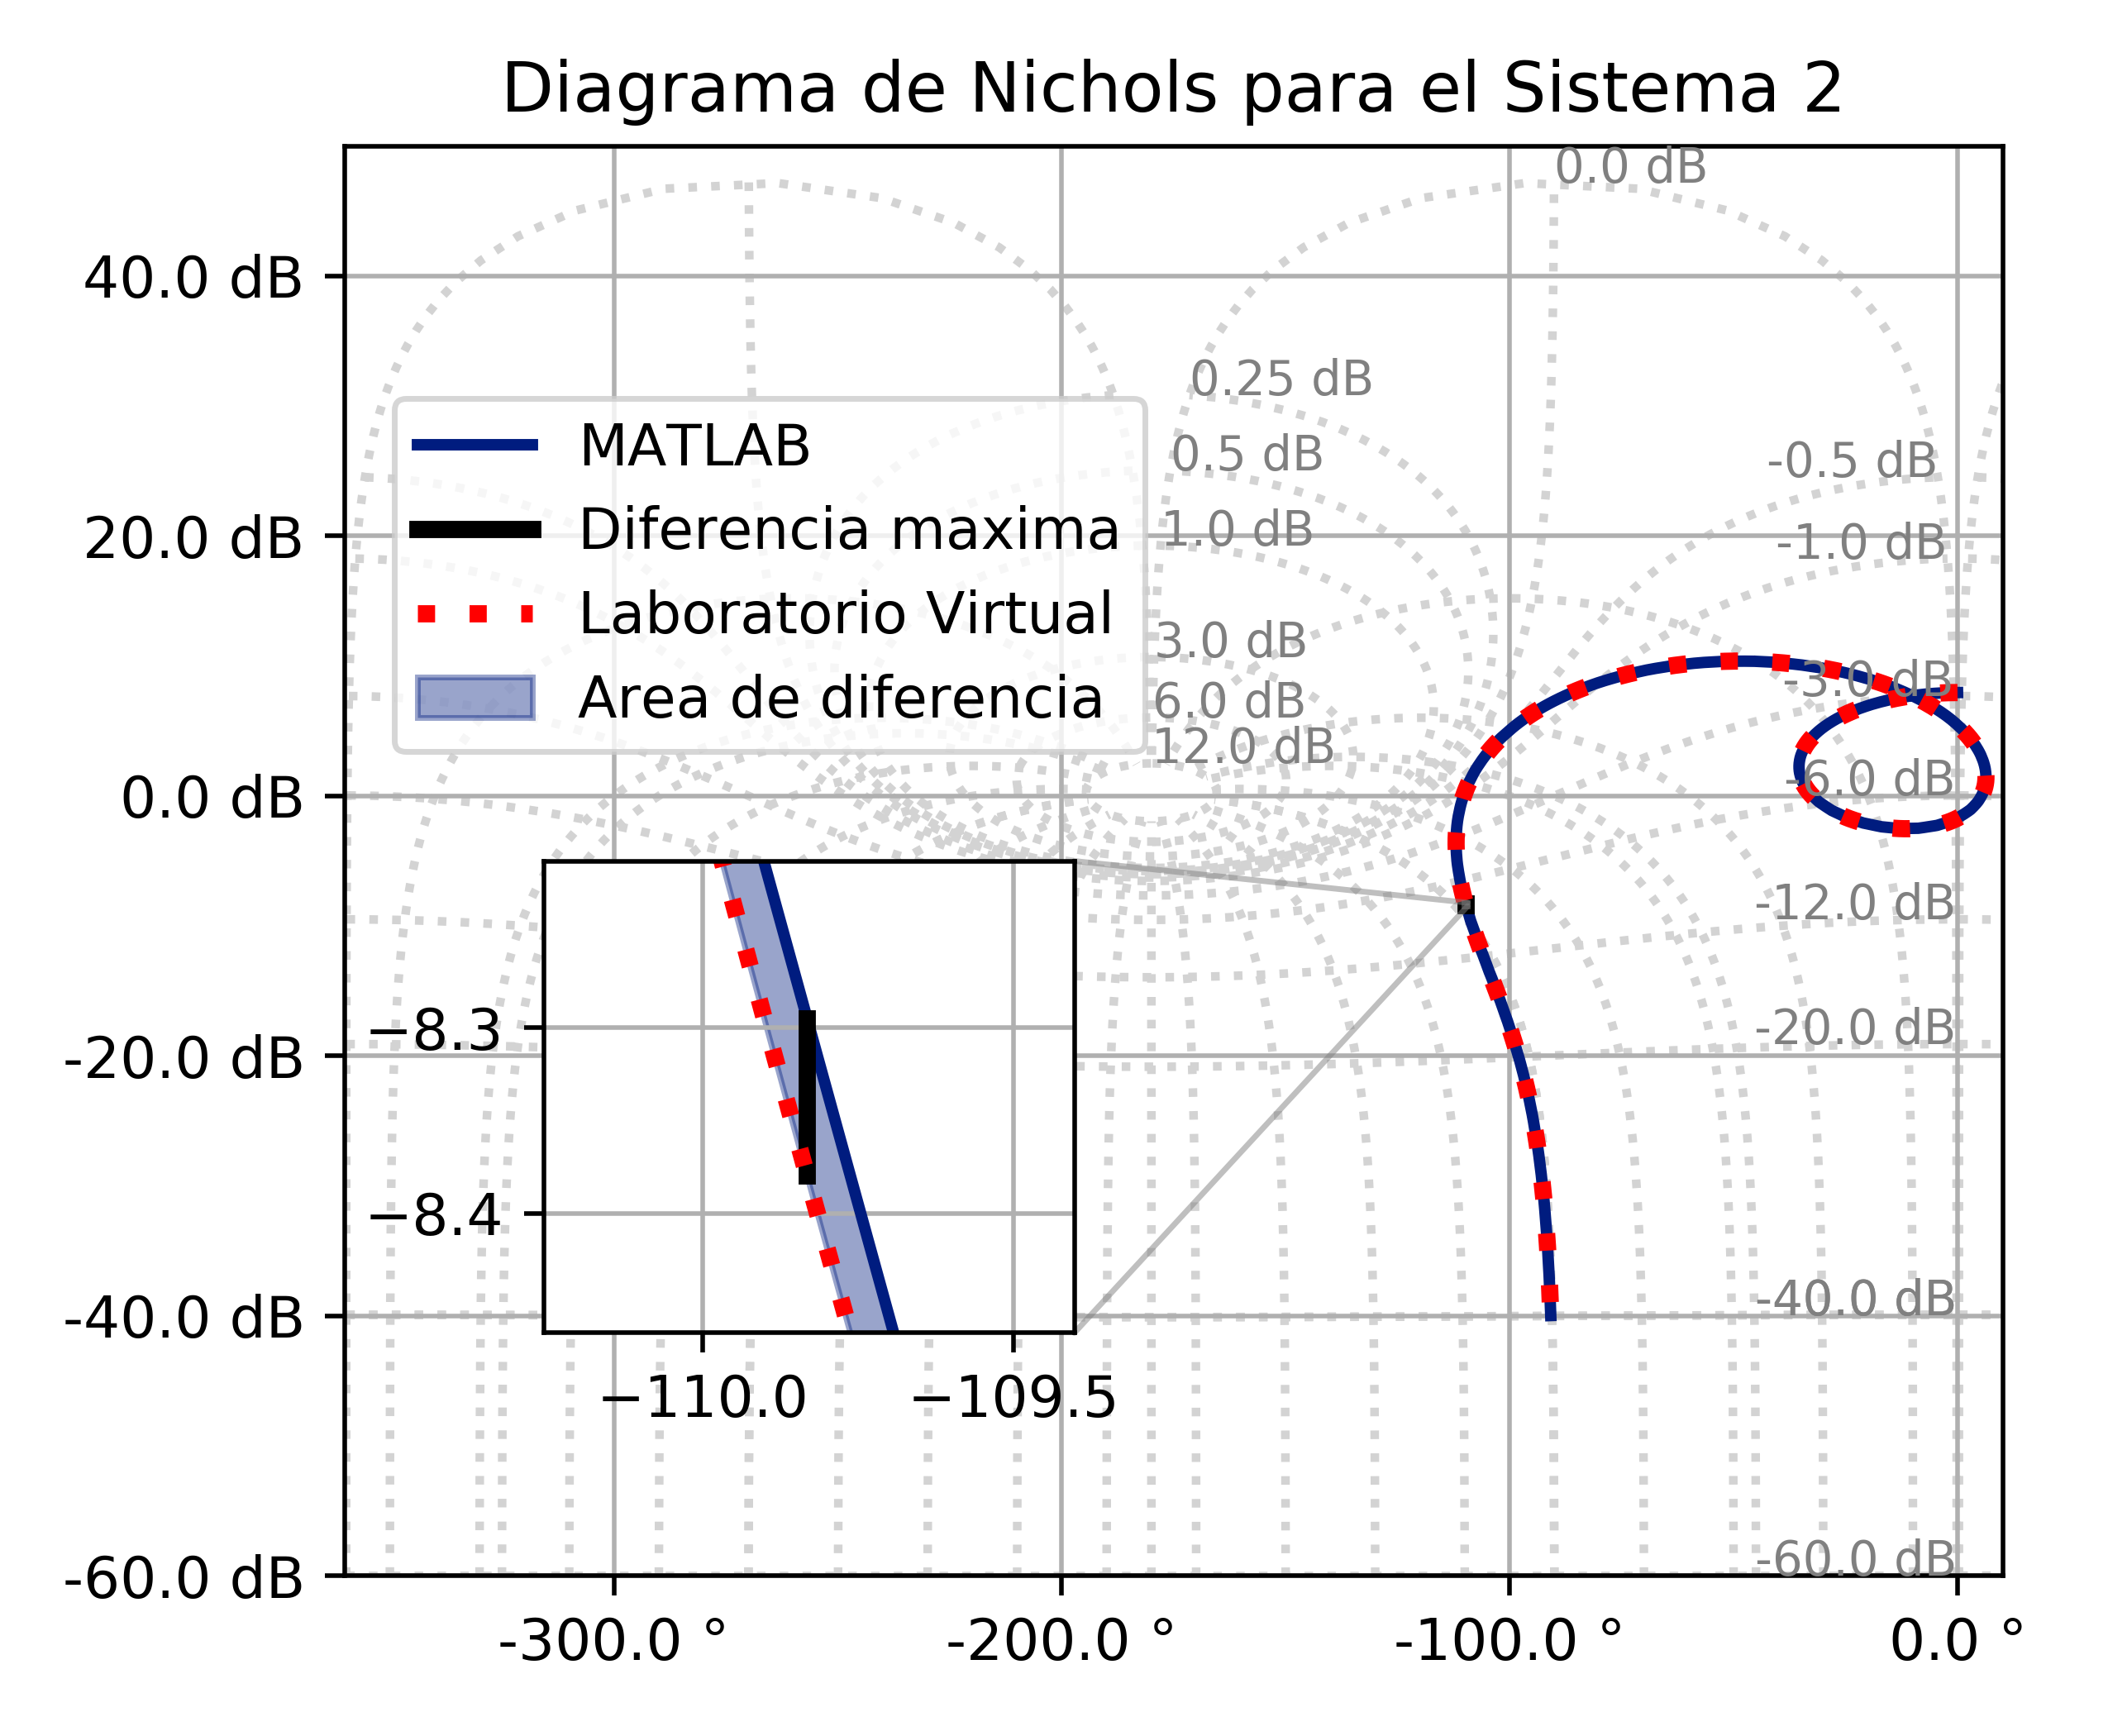
\includegraphics[width=0.43\textwidth,valign=c]{MATLAB/Set2Nichols.png}
            \label{fig:Set2sub}
        \end{subfigure}
        \caption[Comparación de análisis/MATLAB - sistema continuo 2]{\textbf{Comparación de análisis/MATLAB - sistema continuo 2}. Fuente: Elaboración propia. \label{fig:Set2}}
    \end{figure}

    \begin{figure}[htb]
        \centering
        \begin{subfigure}[t]{0.99\textwidth}
            \centering
            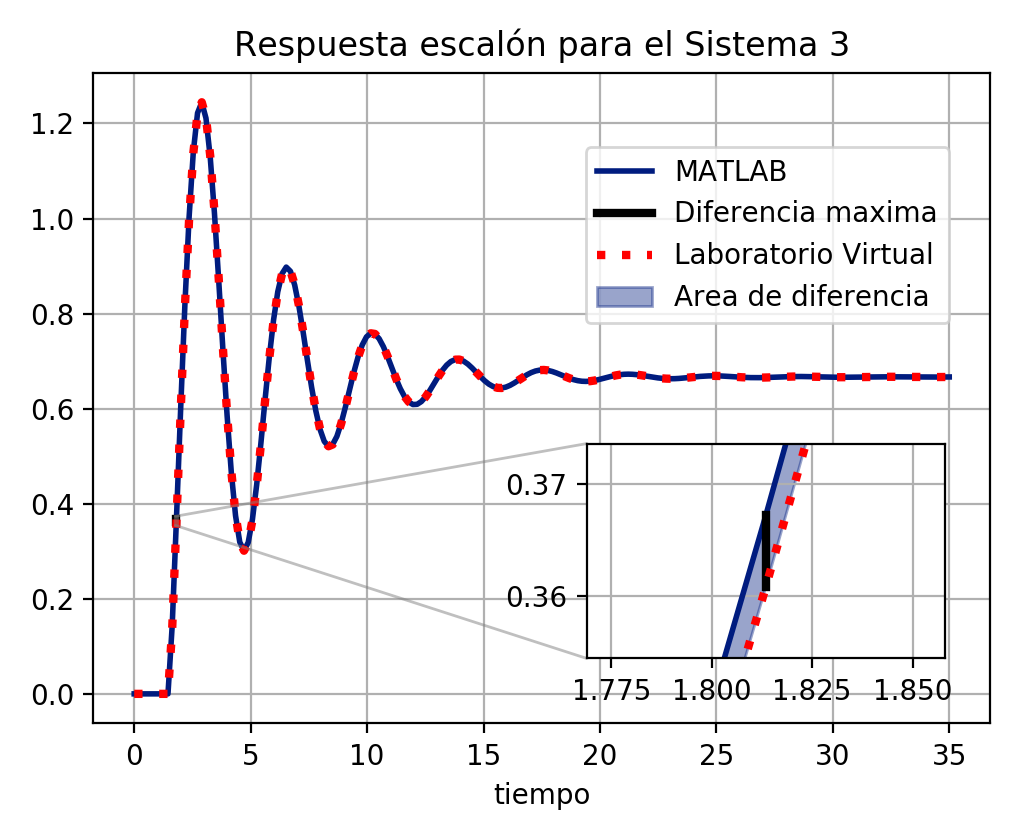
\includegraphics[width=0.49\textwidth,valign=c]{MATLAB/Set3Step.png}
            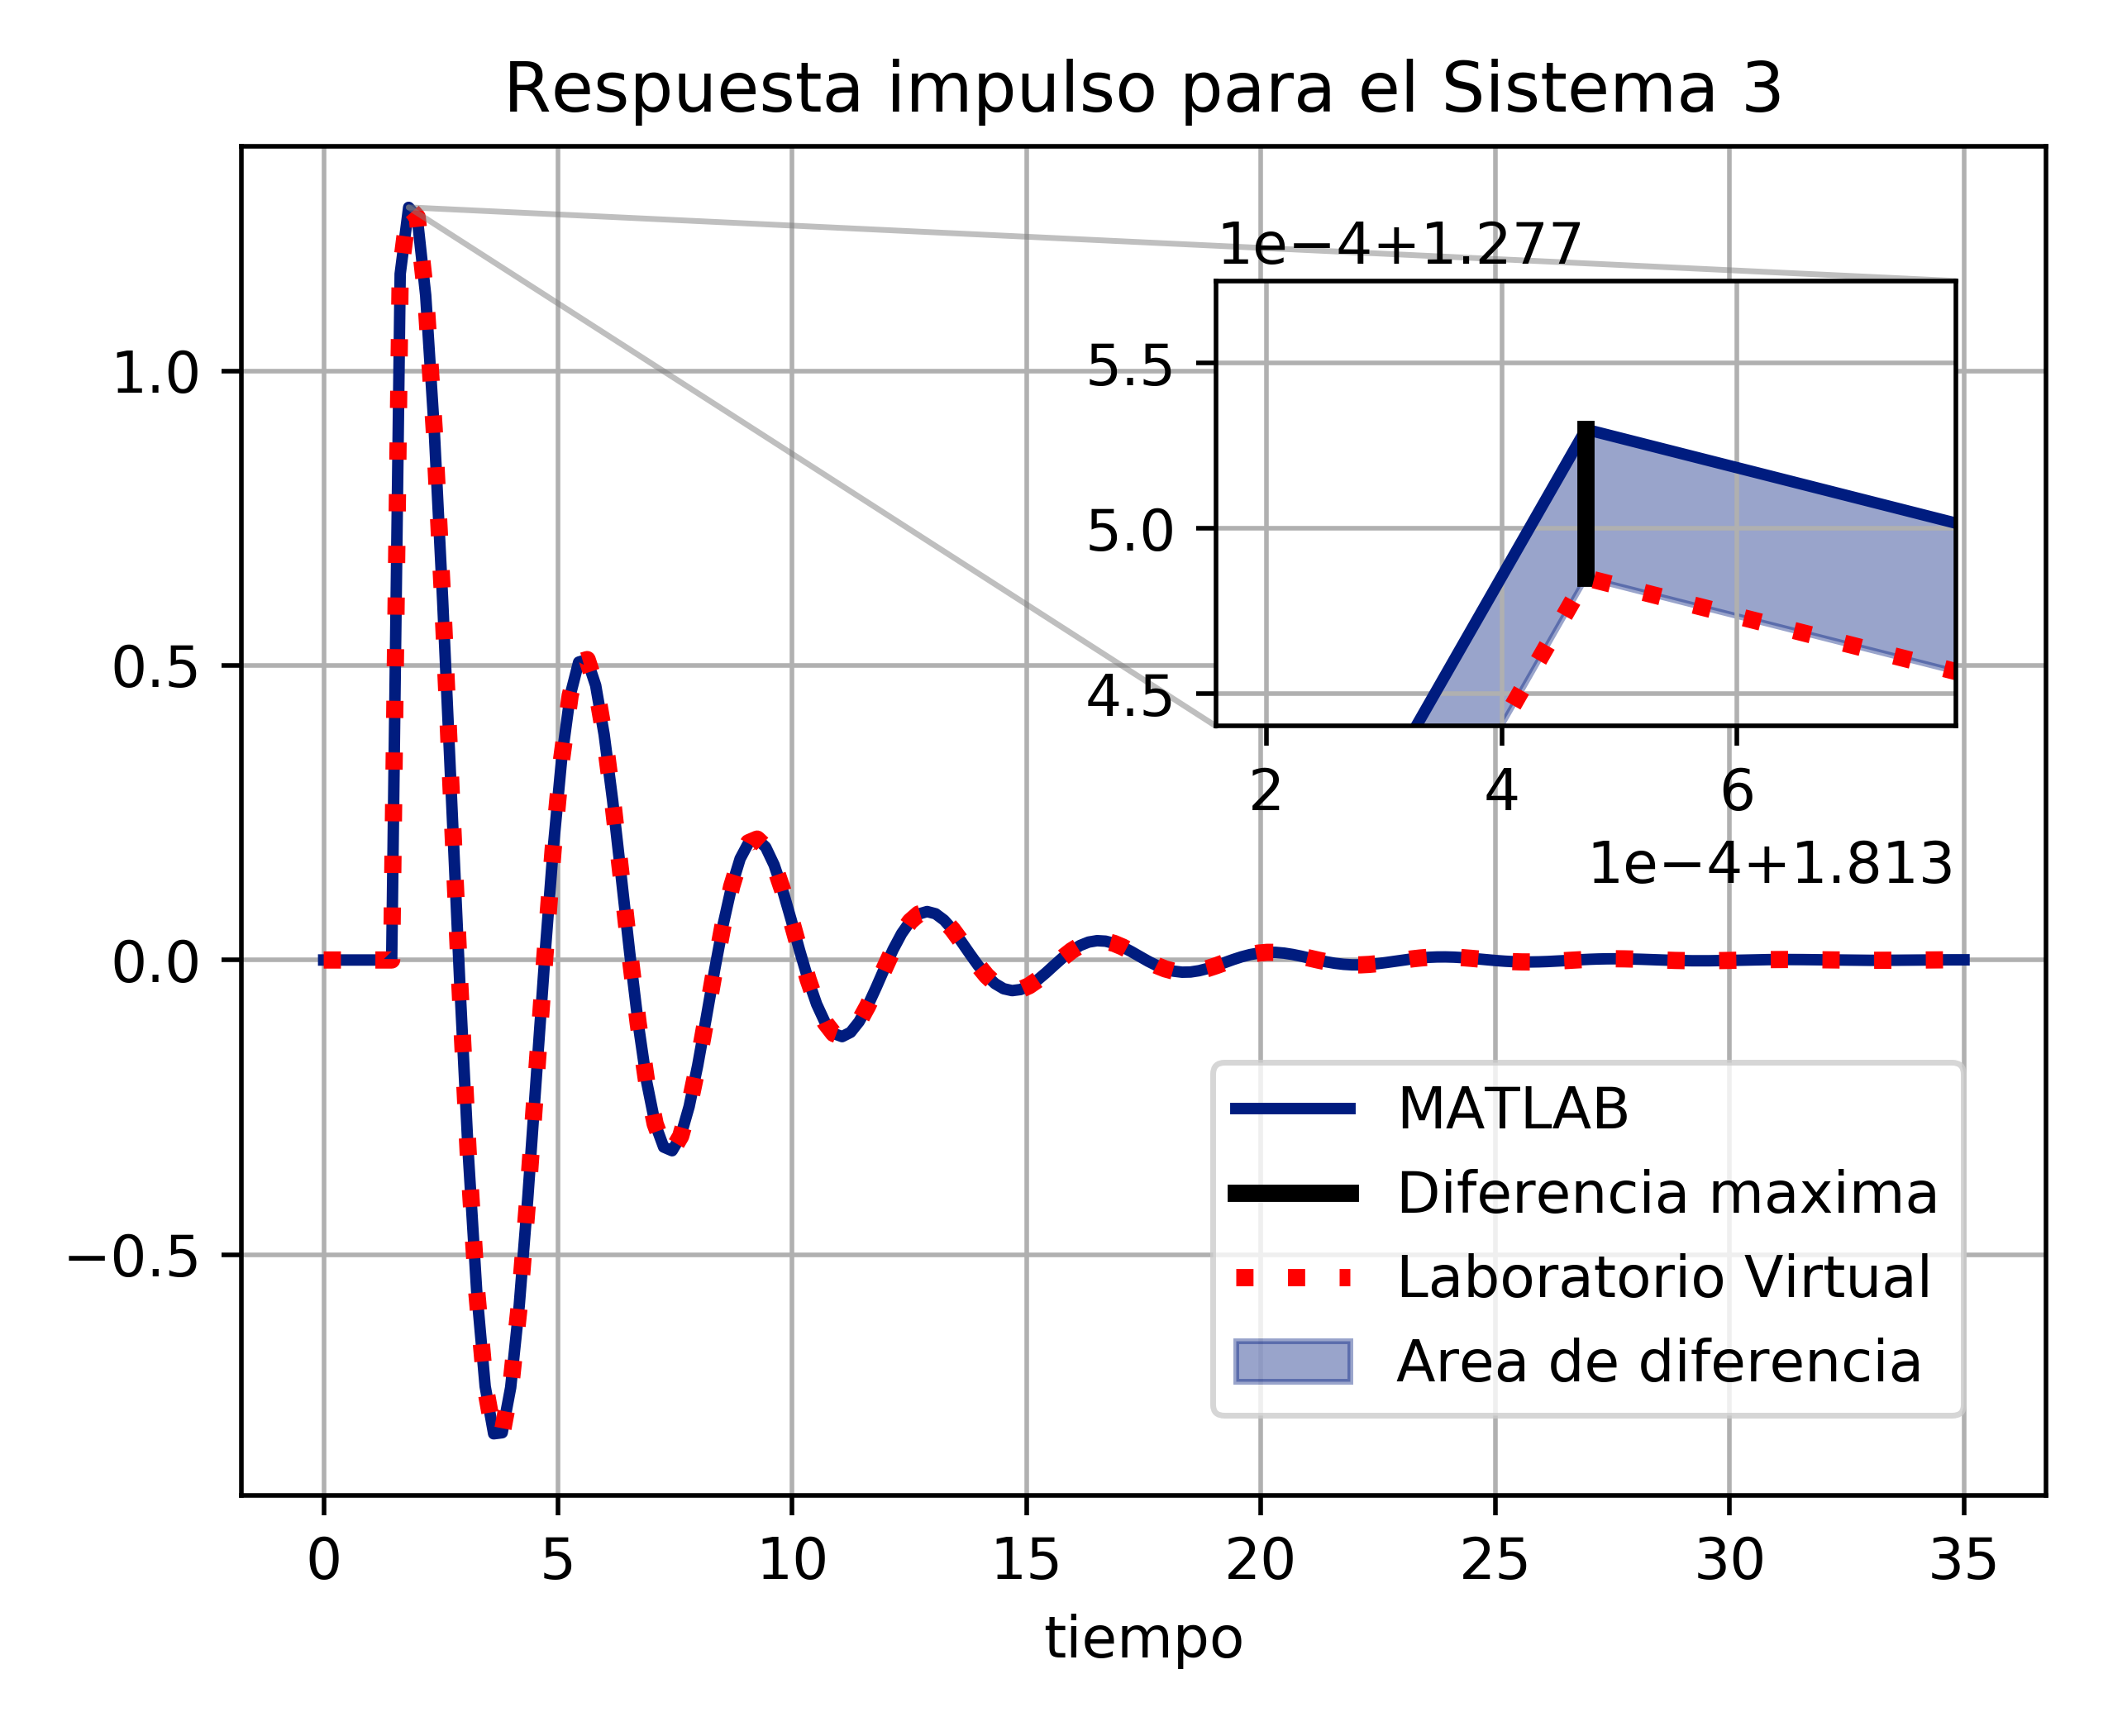
\includegraphics[width=0.49\textwidth,valign=c]{MATLAB/Set3Imp.png}
            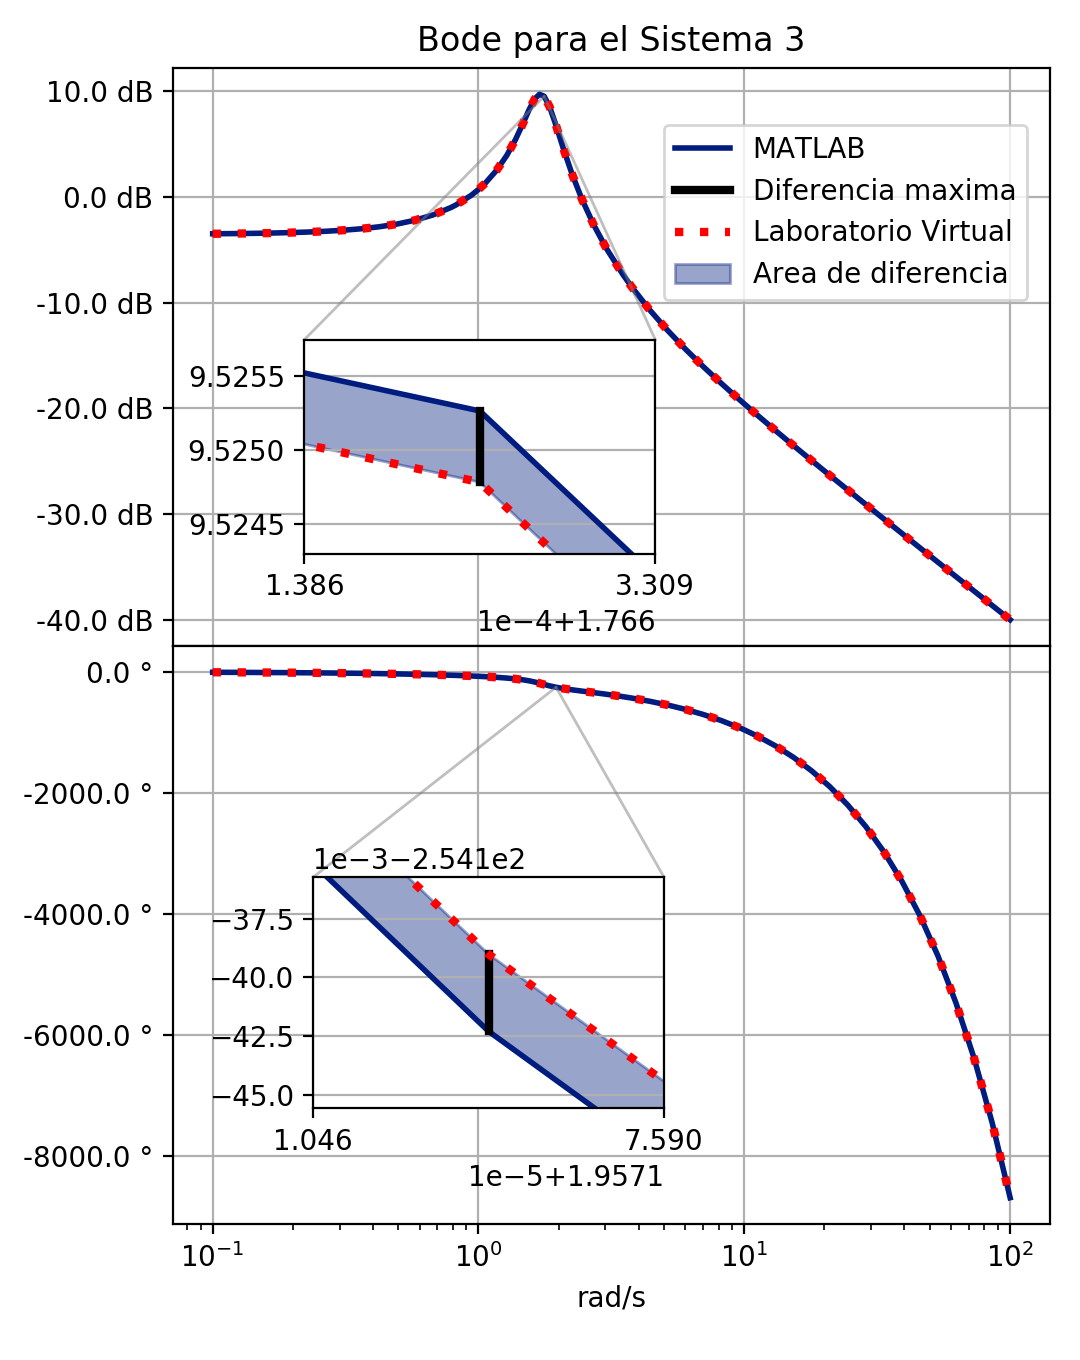
\includegraphics[width=0.49\textwidth,valign=c]{MATLAB/Set3Bode.png}
            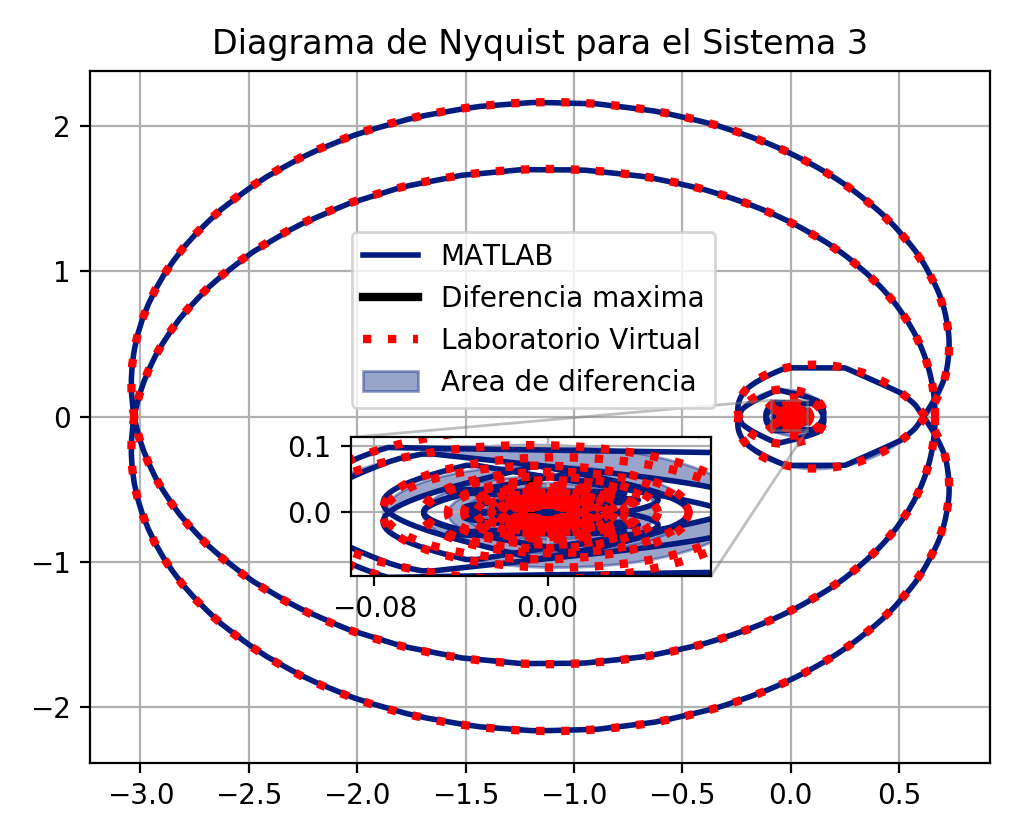
\includegraphics[width=0.49\textwidth,valign=c]{MATLAB/Set3Nyquist.png}
            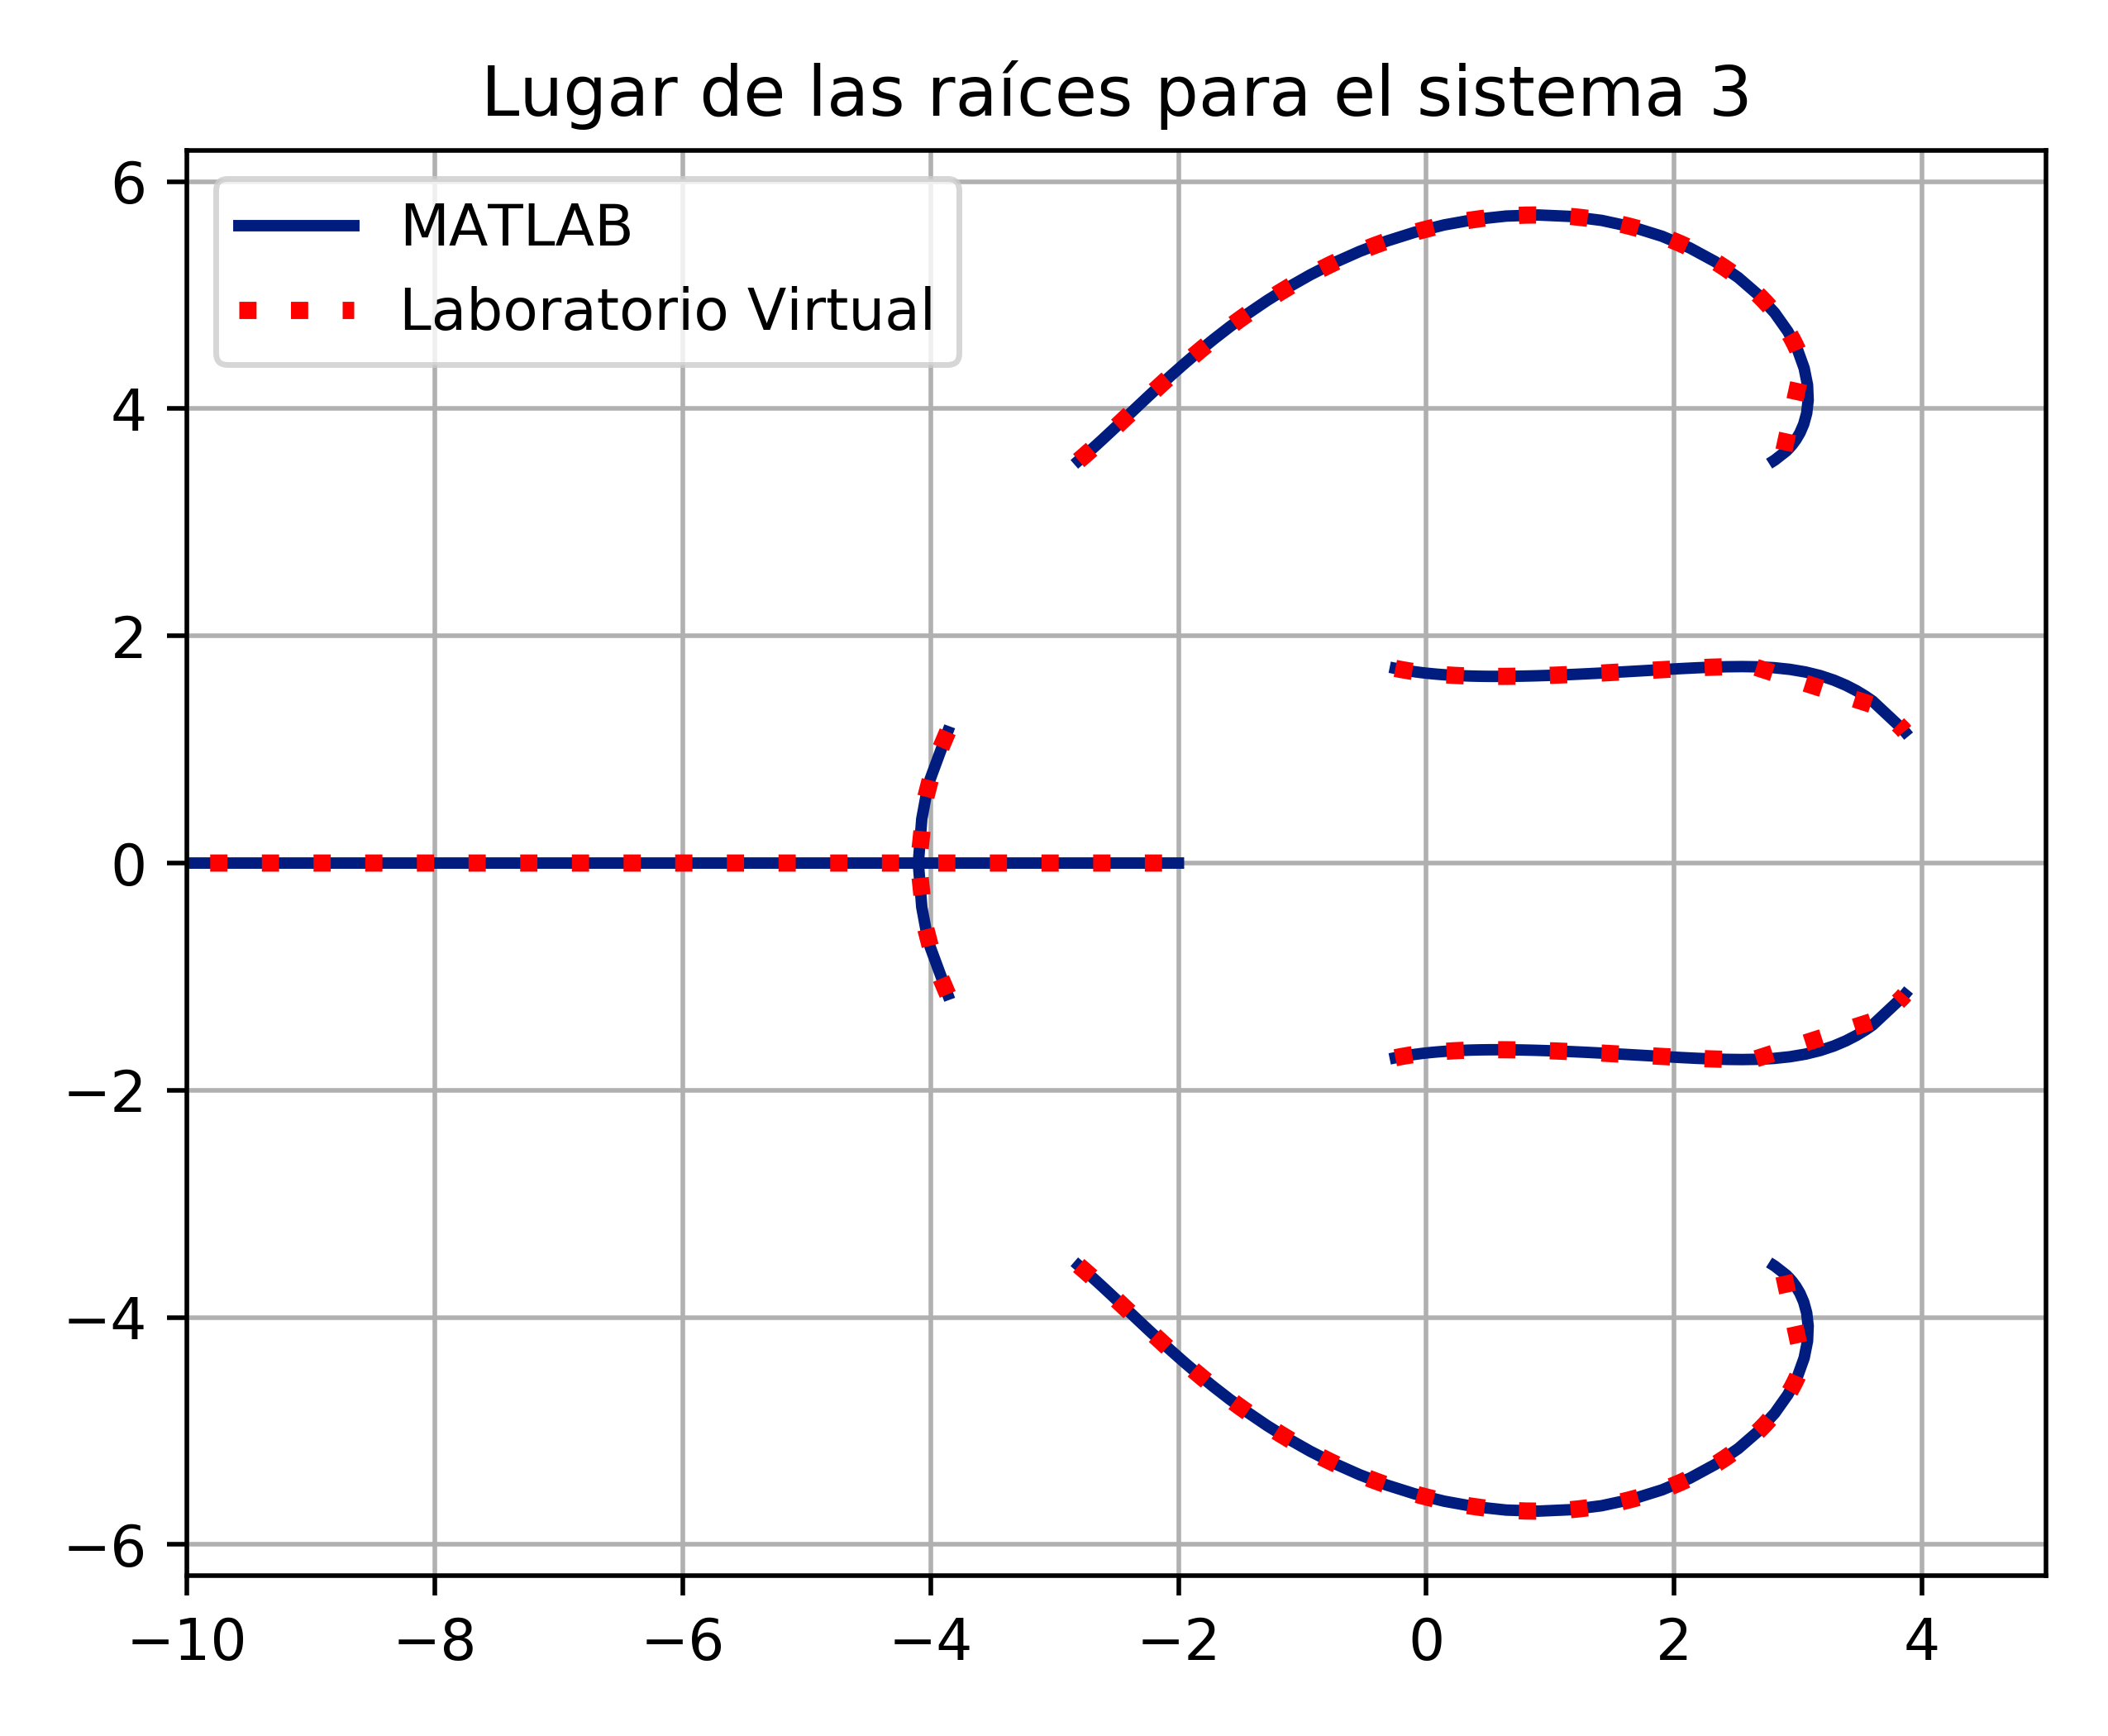
\includegraphics[width=0.49\textwidth,valign=c]{MATLAB/Set3Rlocus.png}
            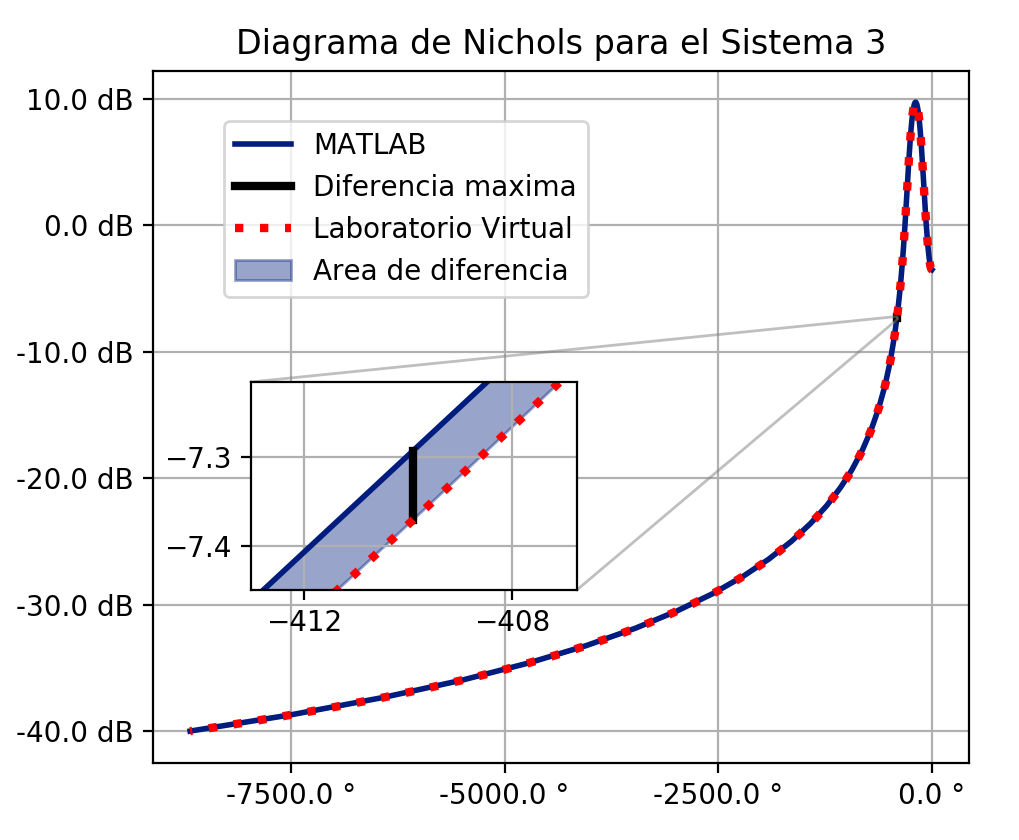
\includegraphics[width=0.49\textwidth,valign=c]{MATLAB/Set3Nichols.png}
            \label{fig:Set3sub}
        \end{subfigure}
        \caption[Comparación de análisis/MATLAB - sistema continuo 3]{\textbf{Comparación de análisis/MATLAB - sistema continuo 3}. Fuente: Elaboración propia. \label{fig:Set3}}
    \end{figure}

    \begin{figure}[htb]
        \centering
        \begin{subfigure}[t]{0.99\textwidth}
            \centering
            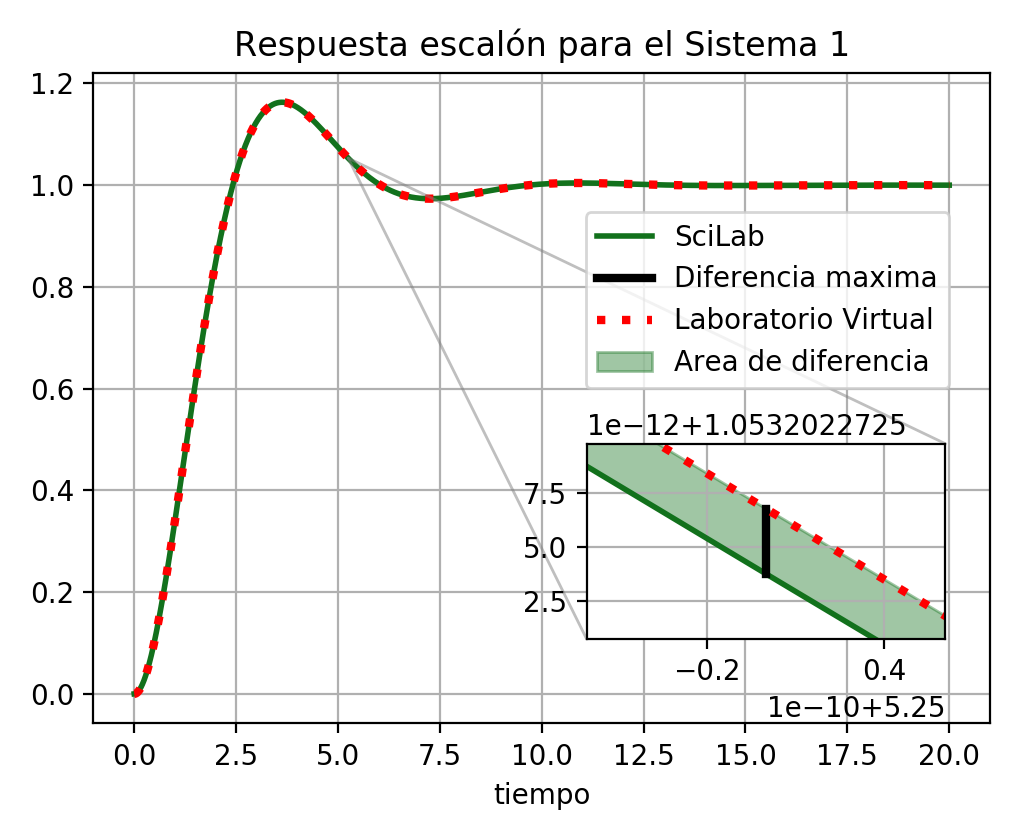
\includegraphics[width=0.49\textwidth,valign=c]{SciLab/ScSet1Step.png}
            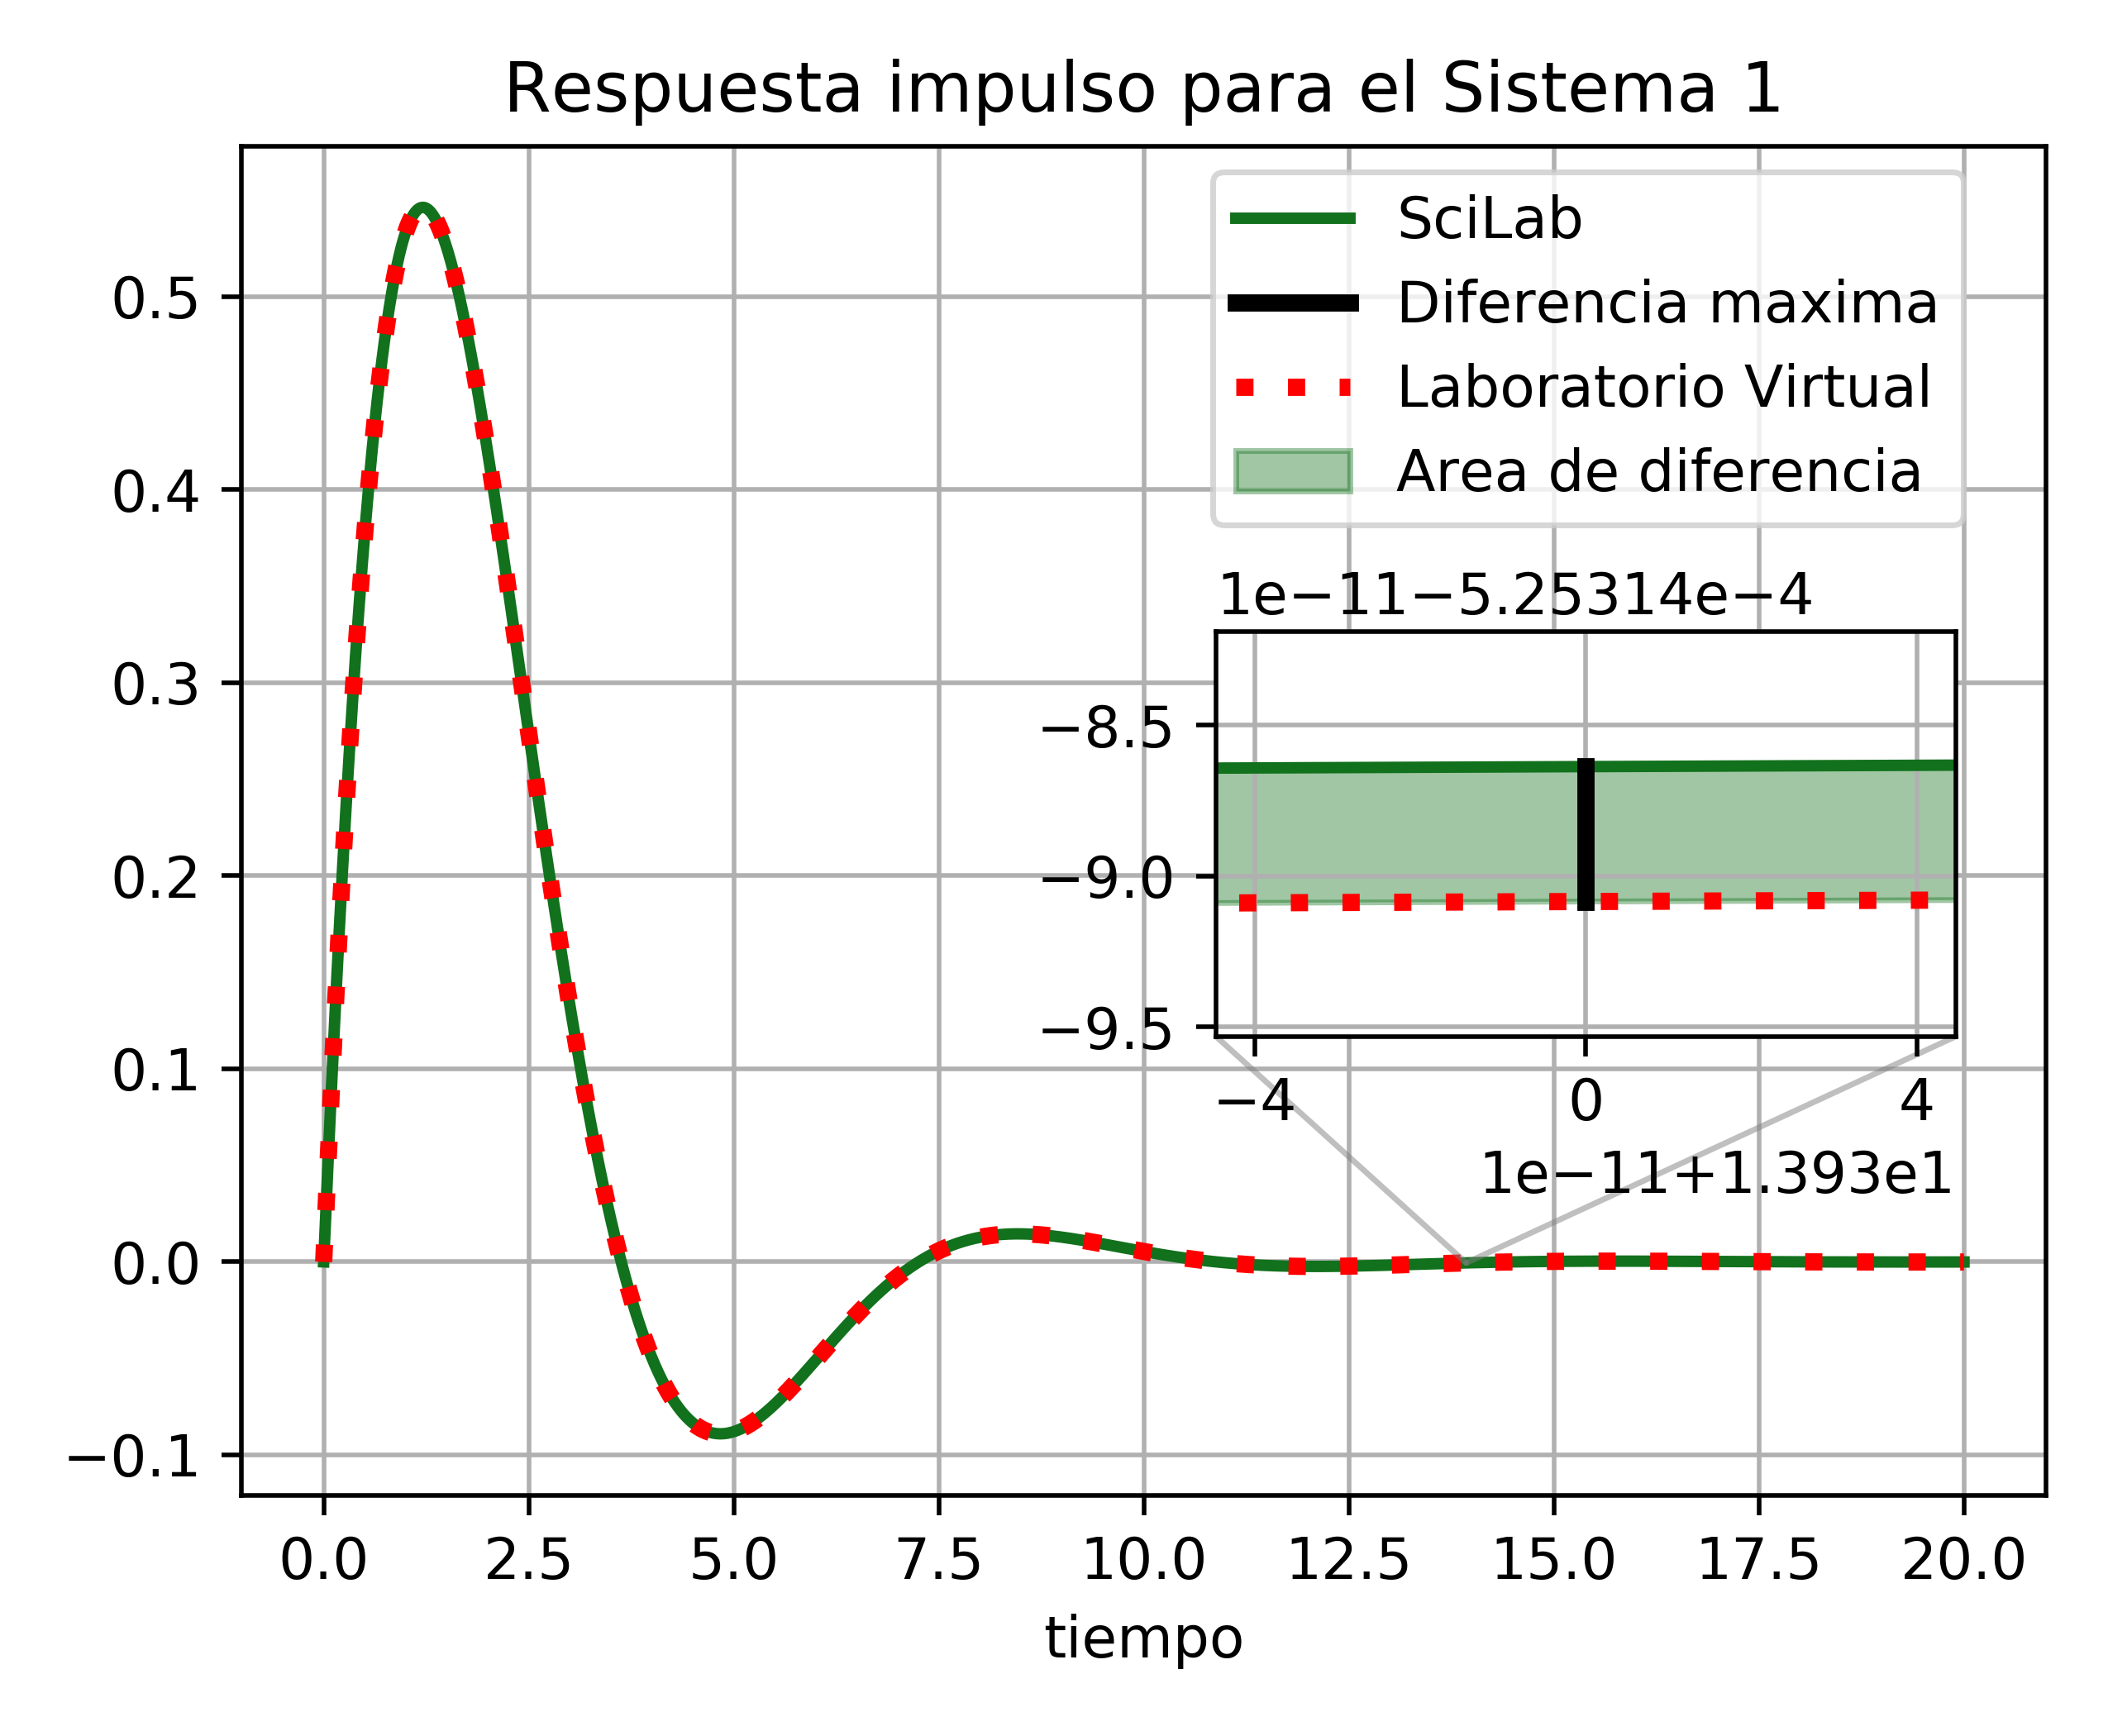
\includegraphics[width=0.49\textwidth,valign=c]{SciLab/ScSet1Imp.png}
            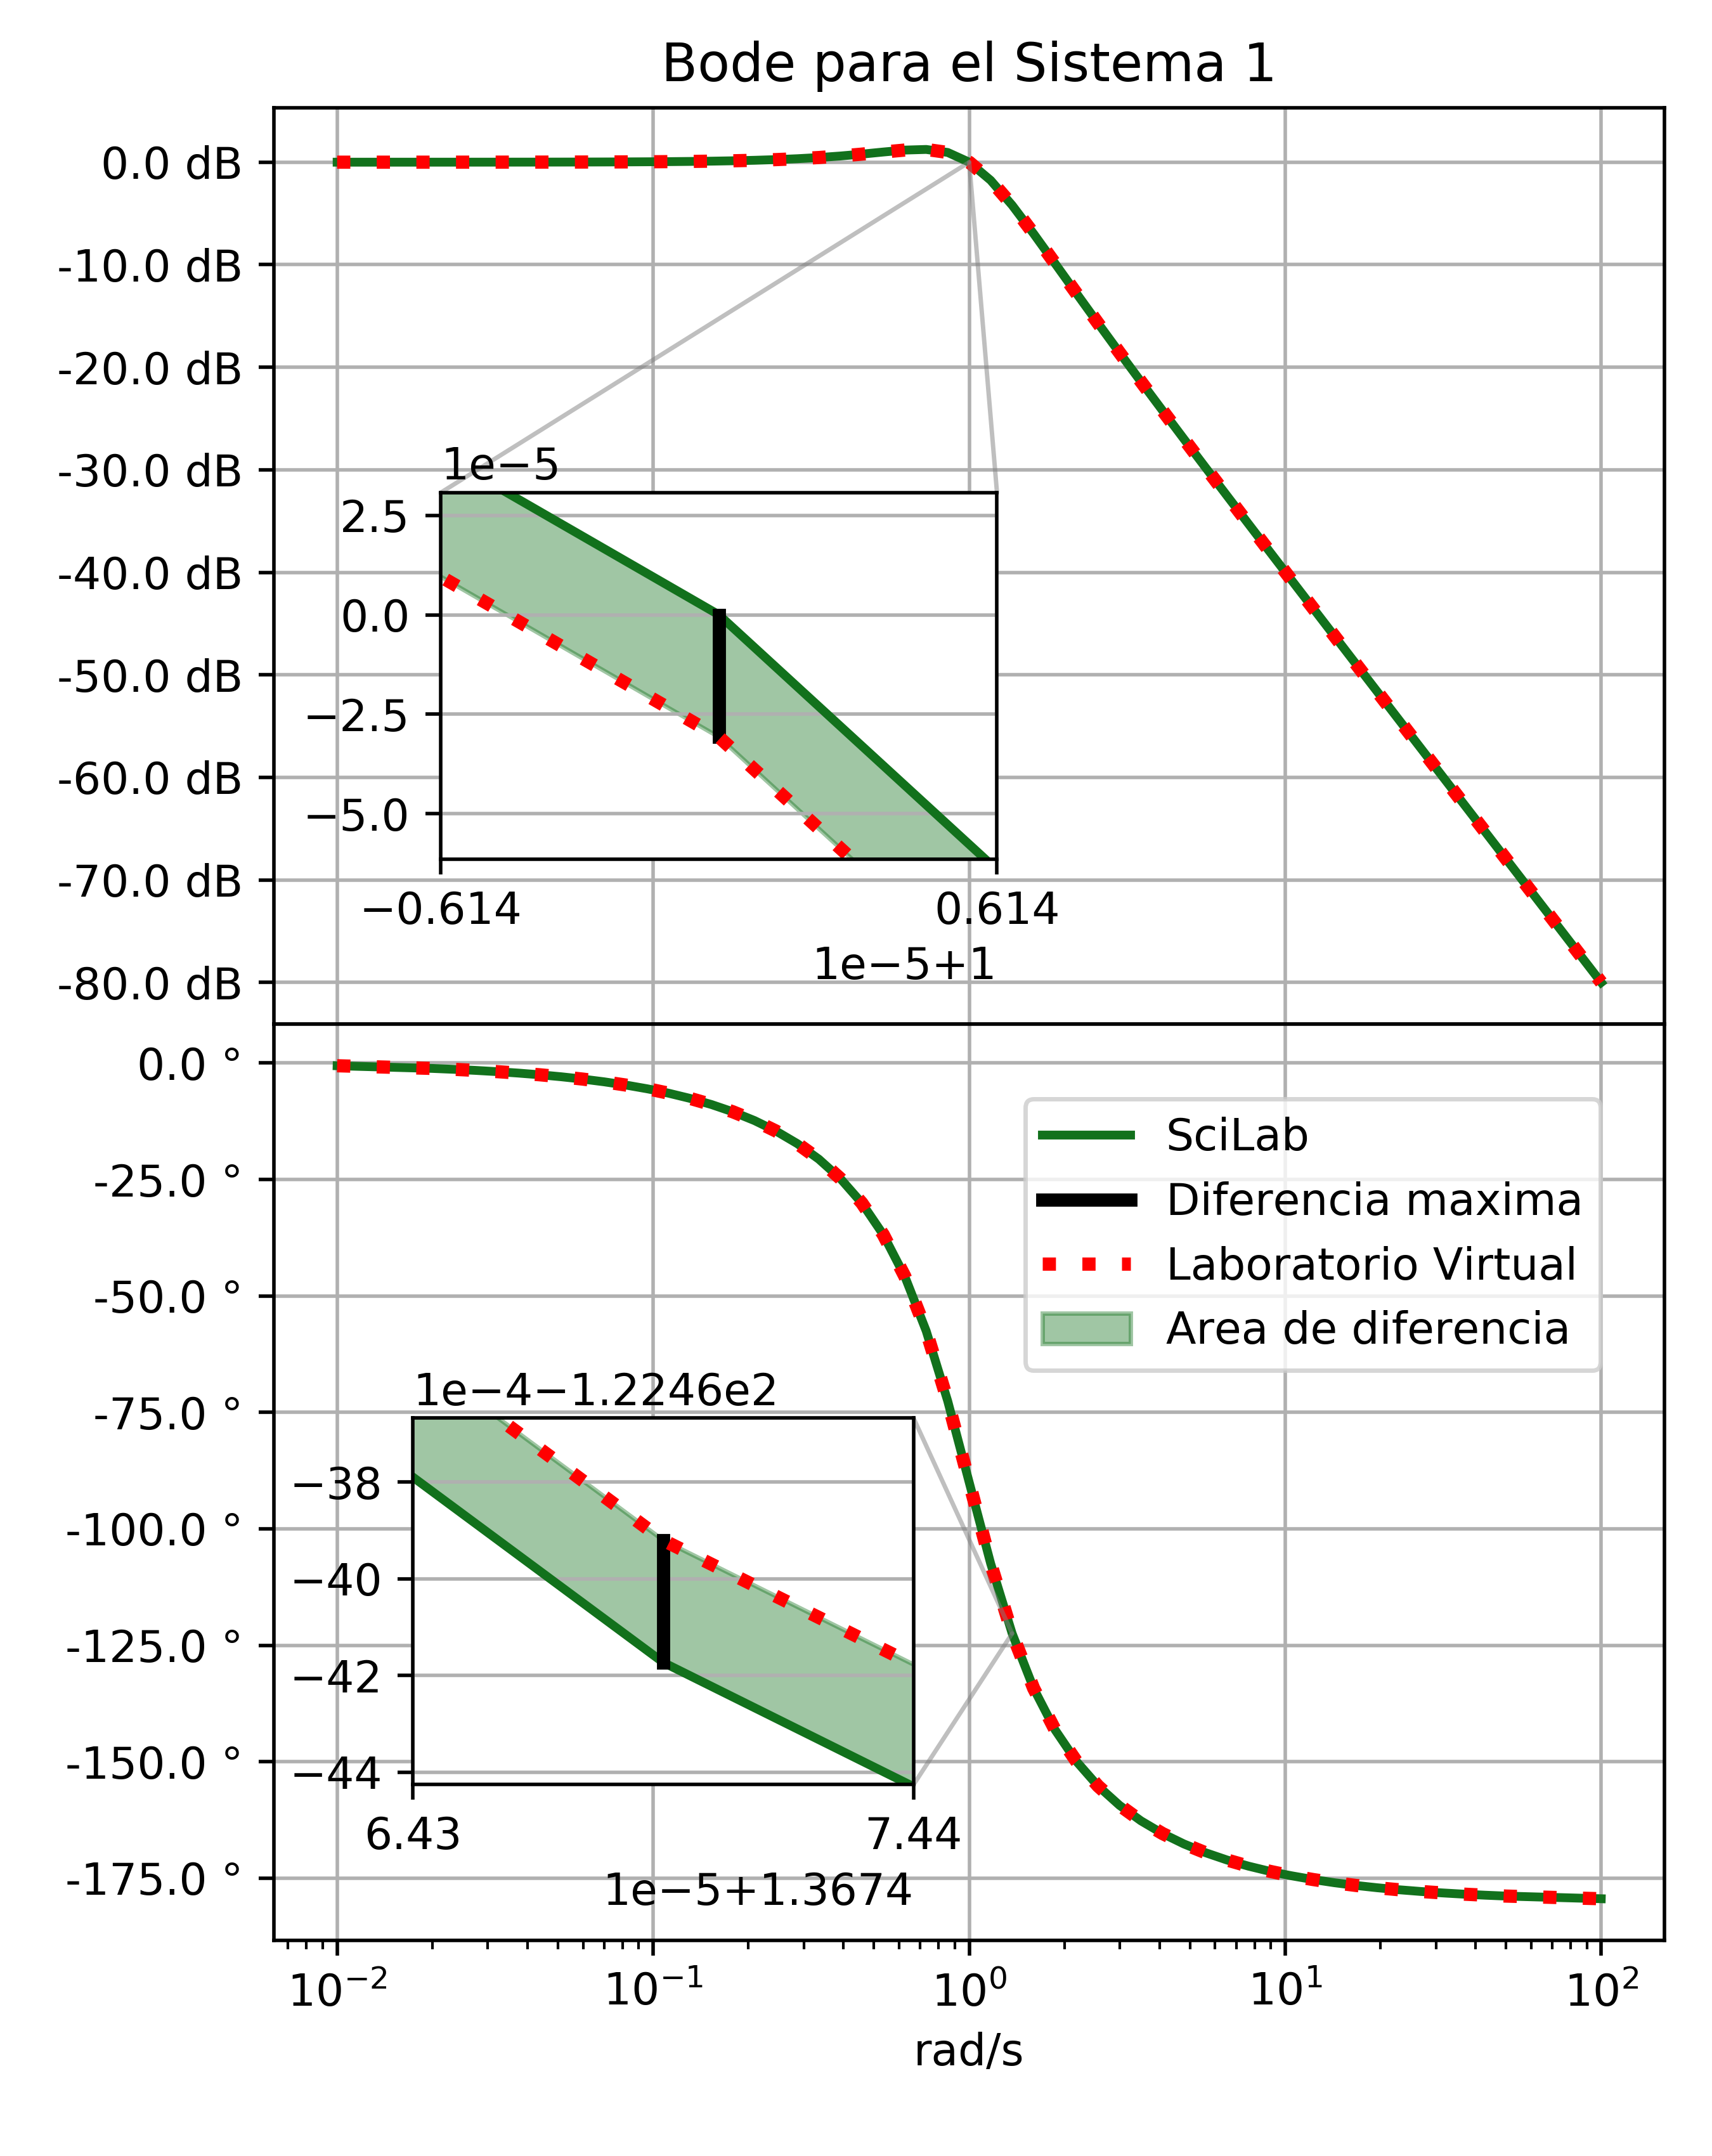
\includegraphics[width=0.49\textwidth,valign=c]{SciLab/ScSet1Bode.png}
            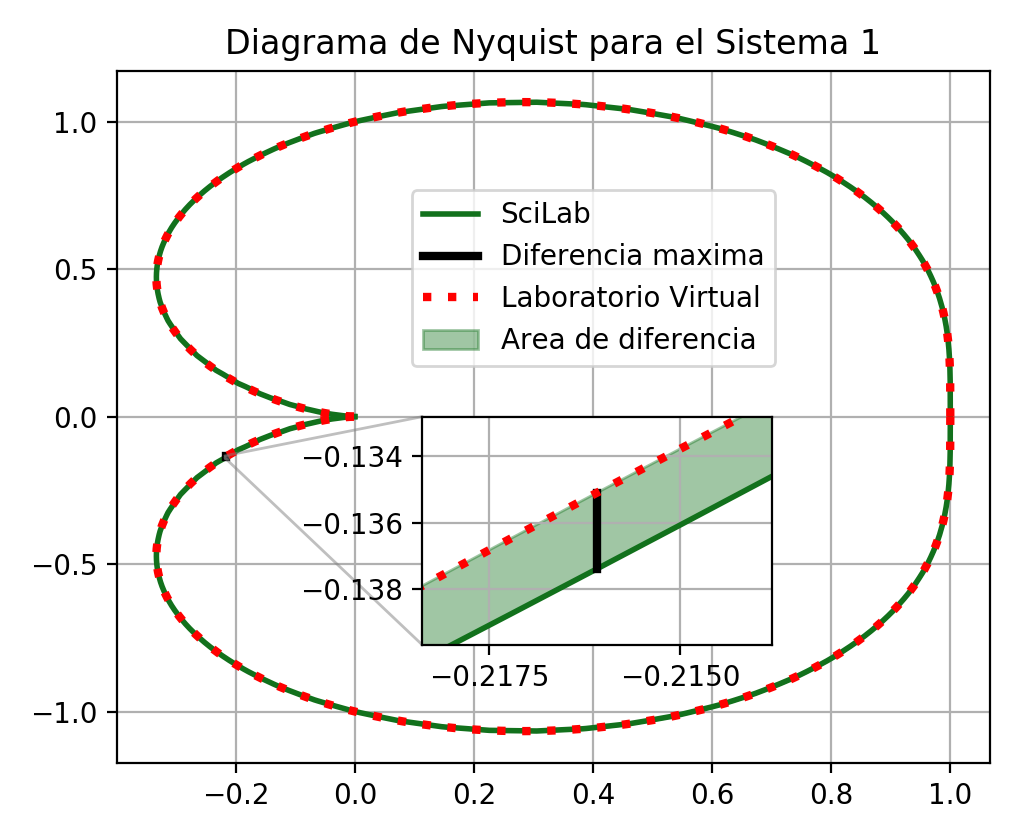
\includegraphics[width=0.49\textwidth,valign=c]{SciLab/ScSet1Nyquist.png}
            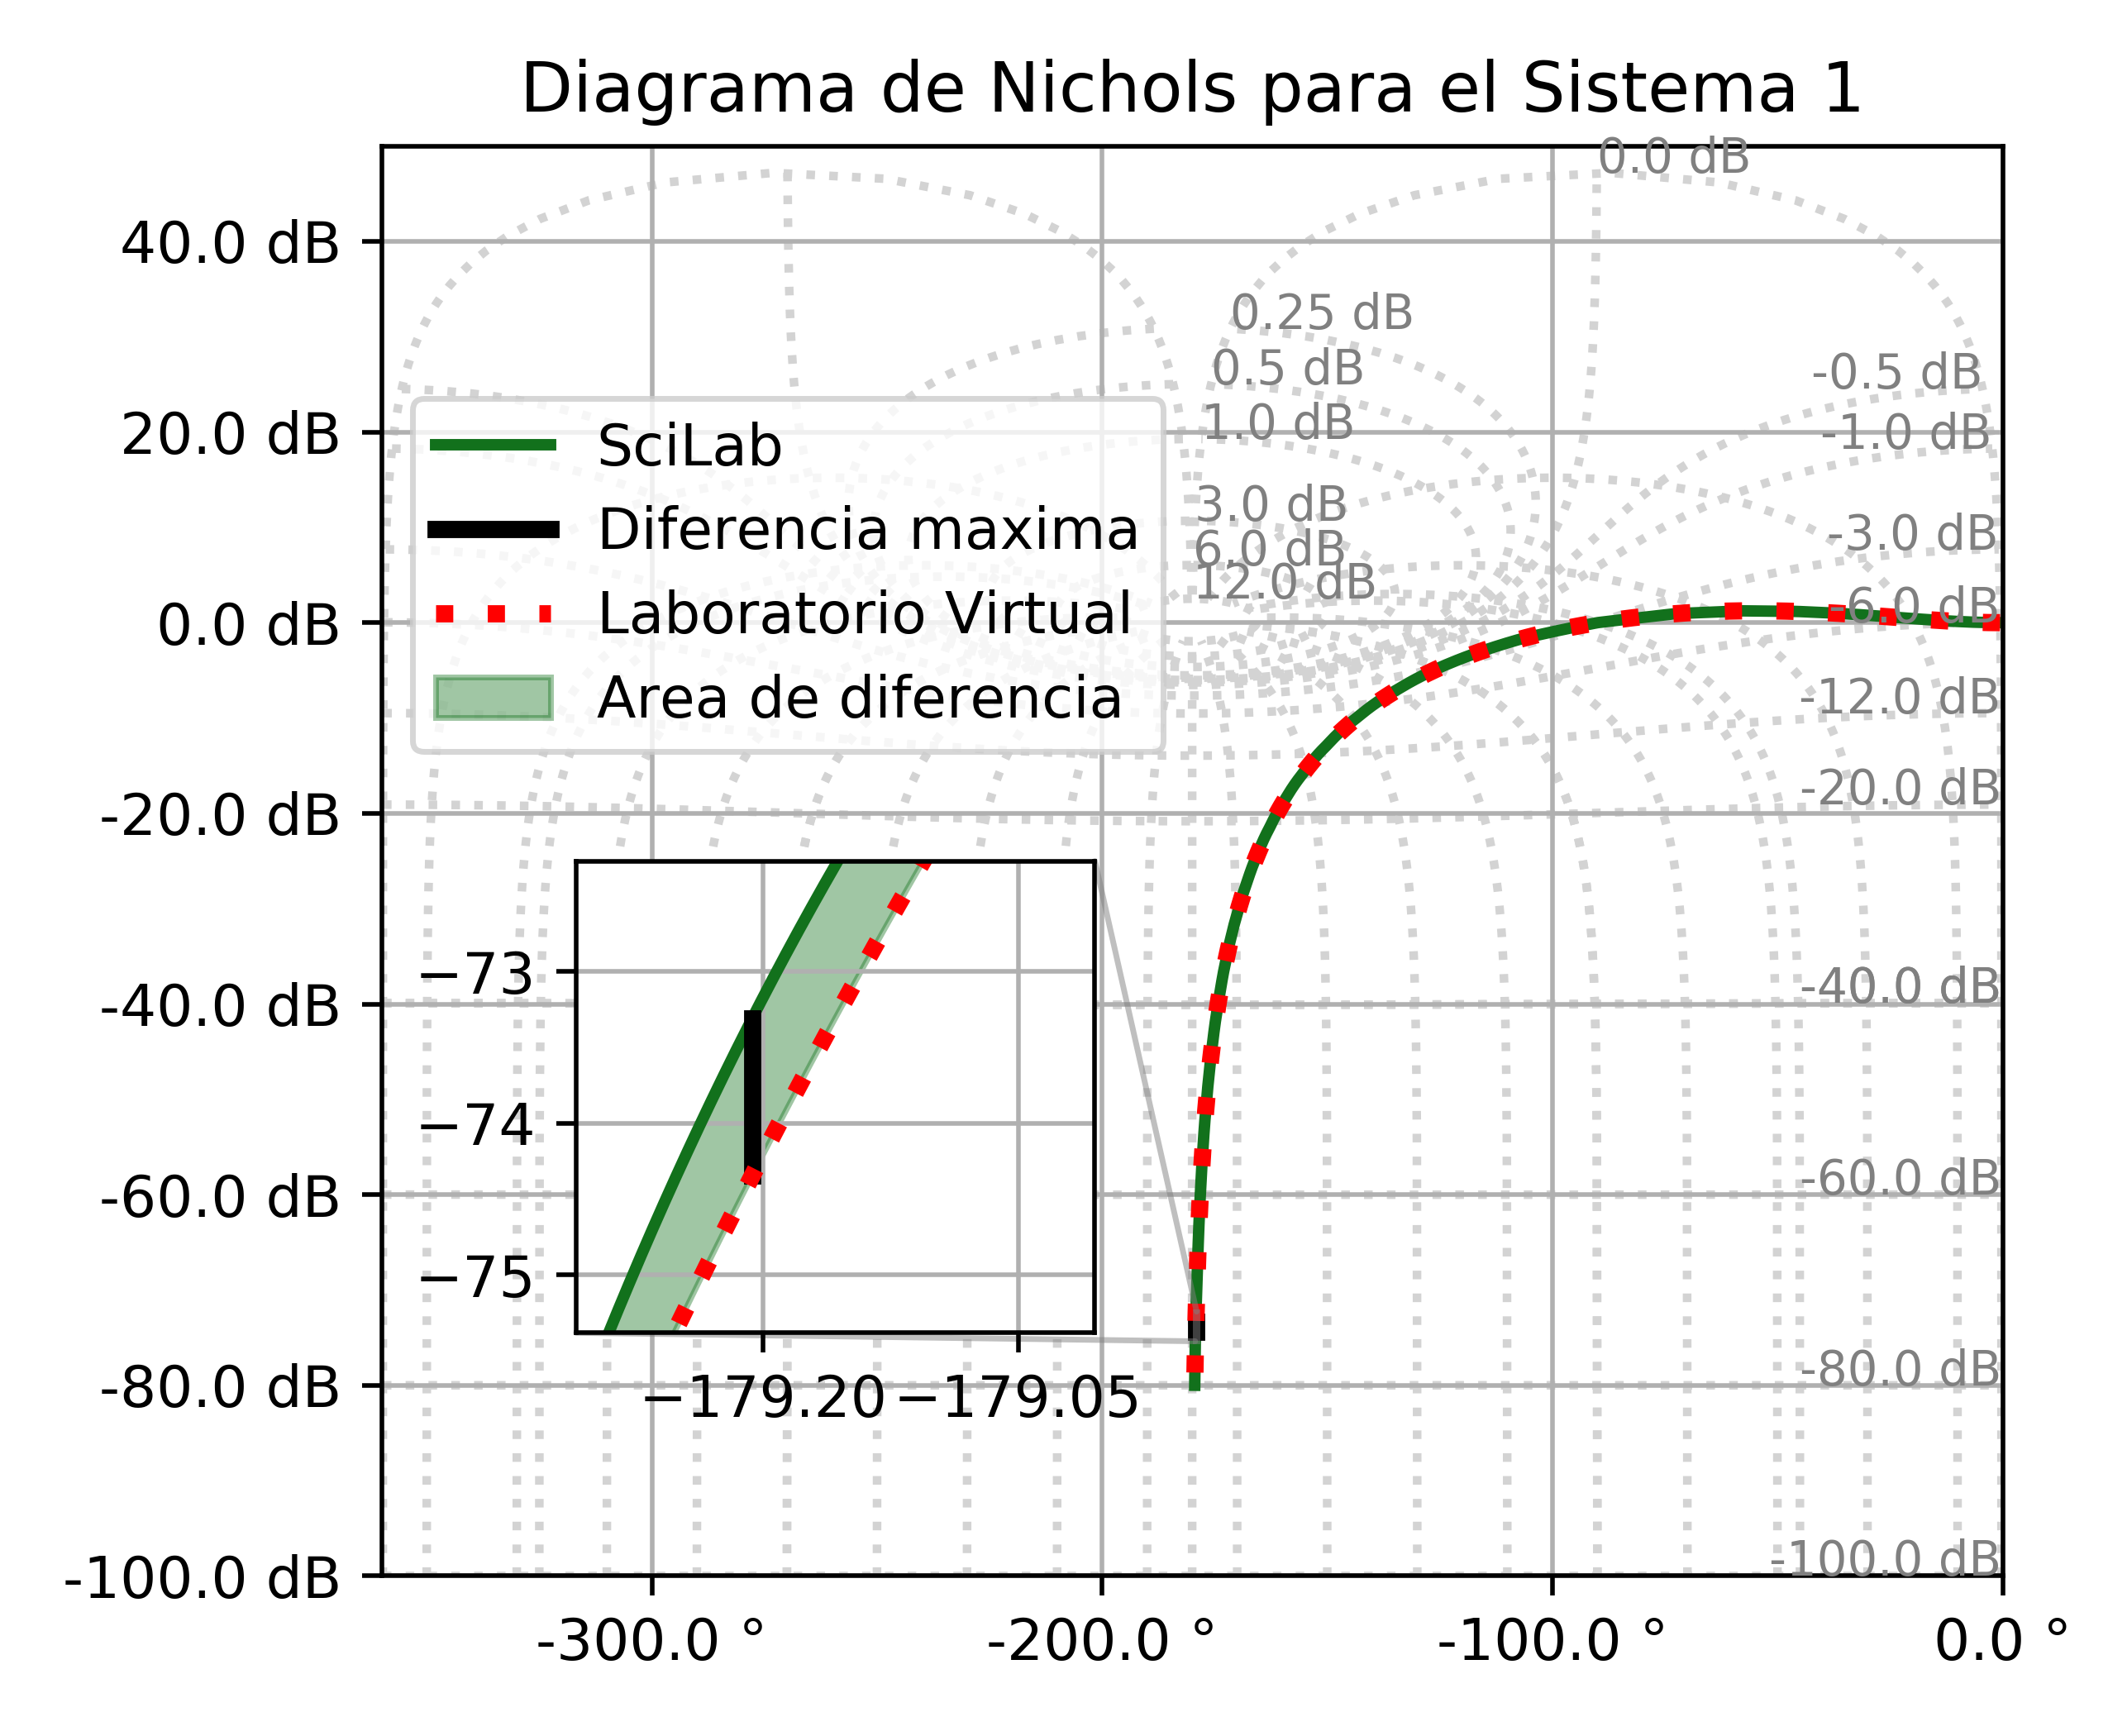
\includegraphics[width=0.49\textwidth,valign=c]{SciLab/ScSet1Nichols.png}
            \label{fig:ScSet1sub}
        \end{subfigure}
        \caption[Comparación de análisis/SciLab - sistema continuo 1]{\textbf{Comparación de análisis/SciLab - sistema continuo 1}. Fuente: Elaboración propia. \label{fig:ScSet1}}
    \end{figure}

    \begin{figure}[htb]
        \centering
        \begin{subfigure}[t]{0.99\textwidth}
            \centering
            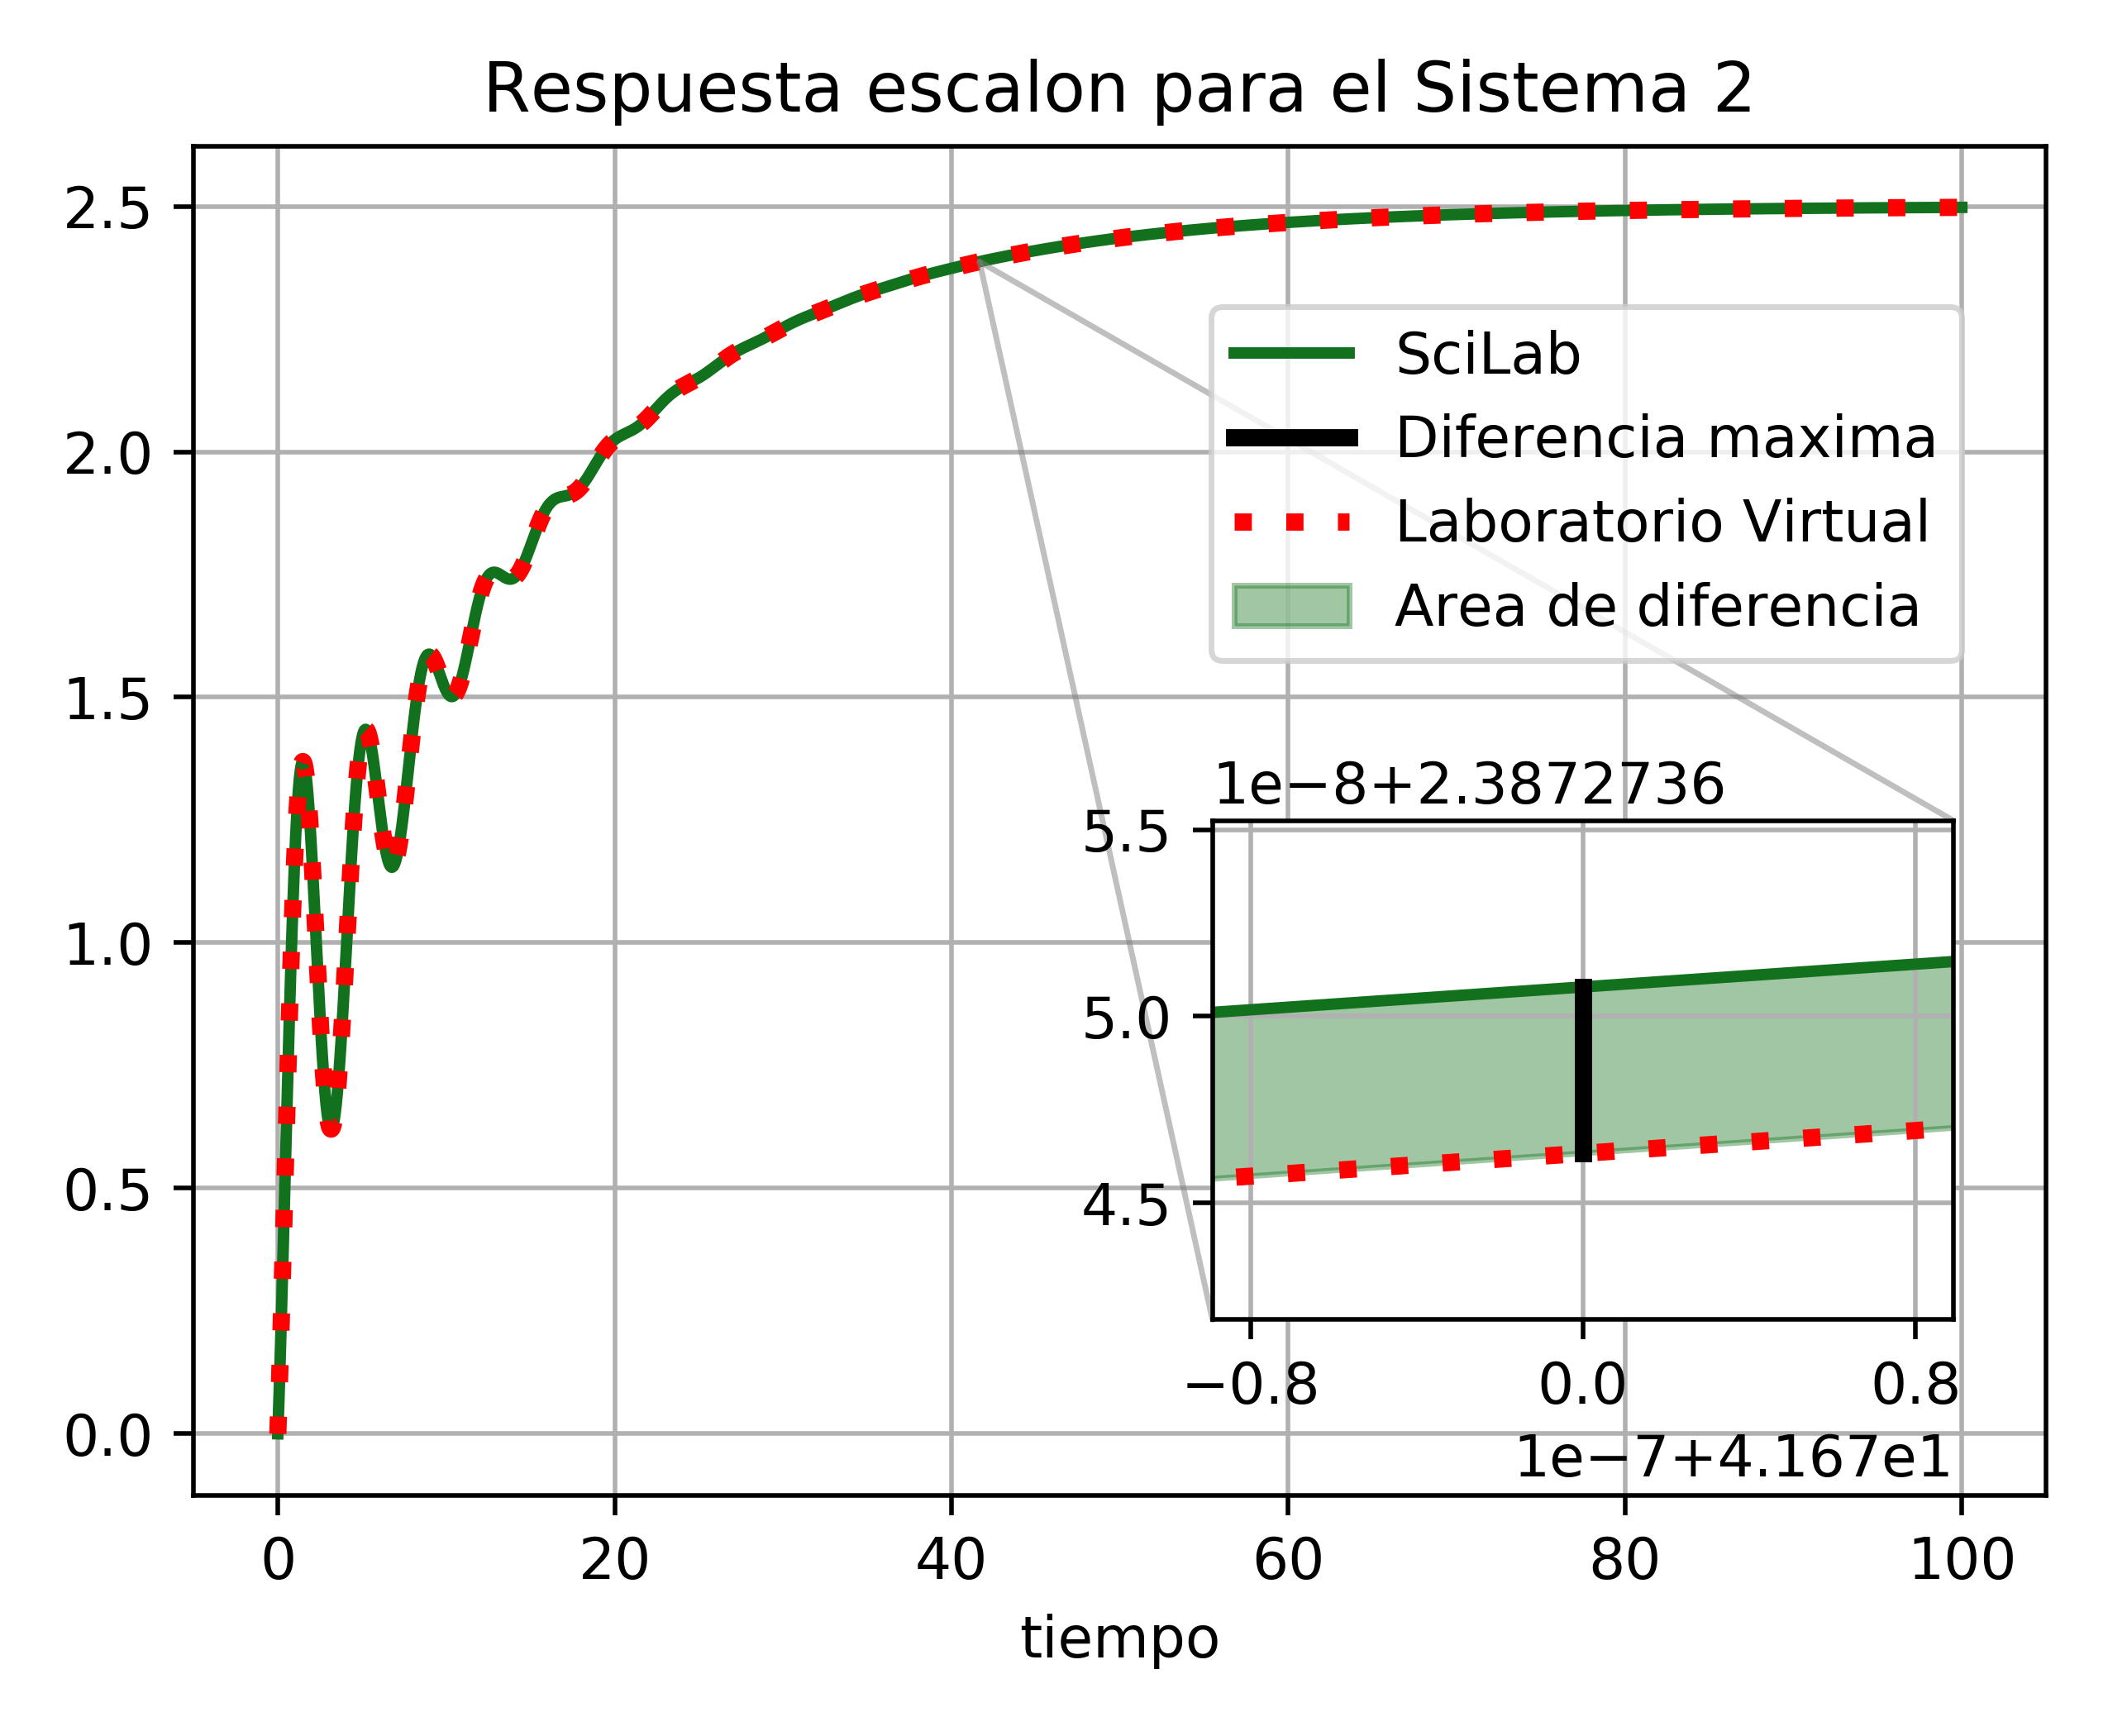
\includegraphics[width=0.49\textwidth,valign=c]{SciLab/ScSet2Step.png}
            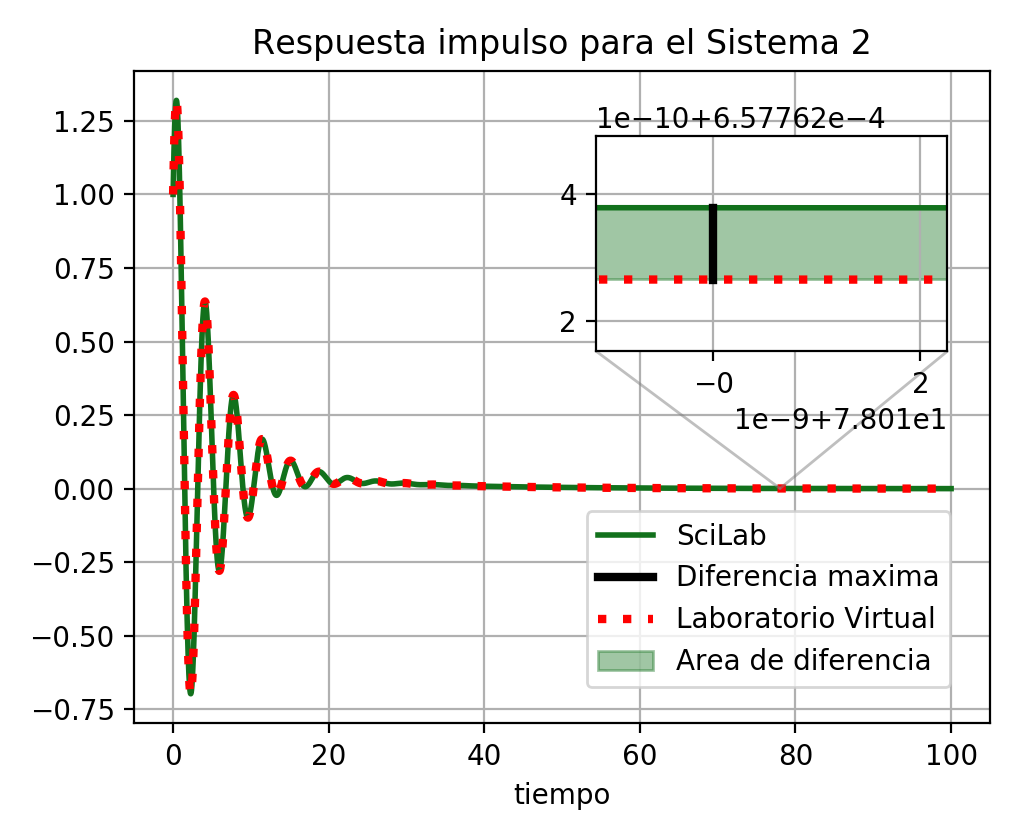
\includegraphics[width=0.49\textwidth,valign=c]{SciLab/ScSet2Imp.png}
            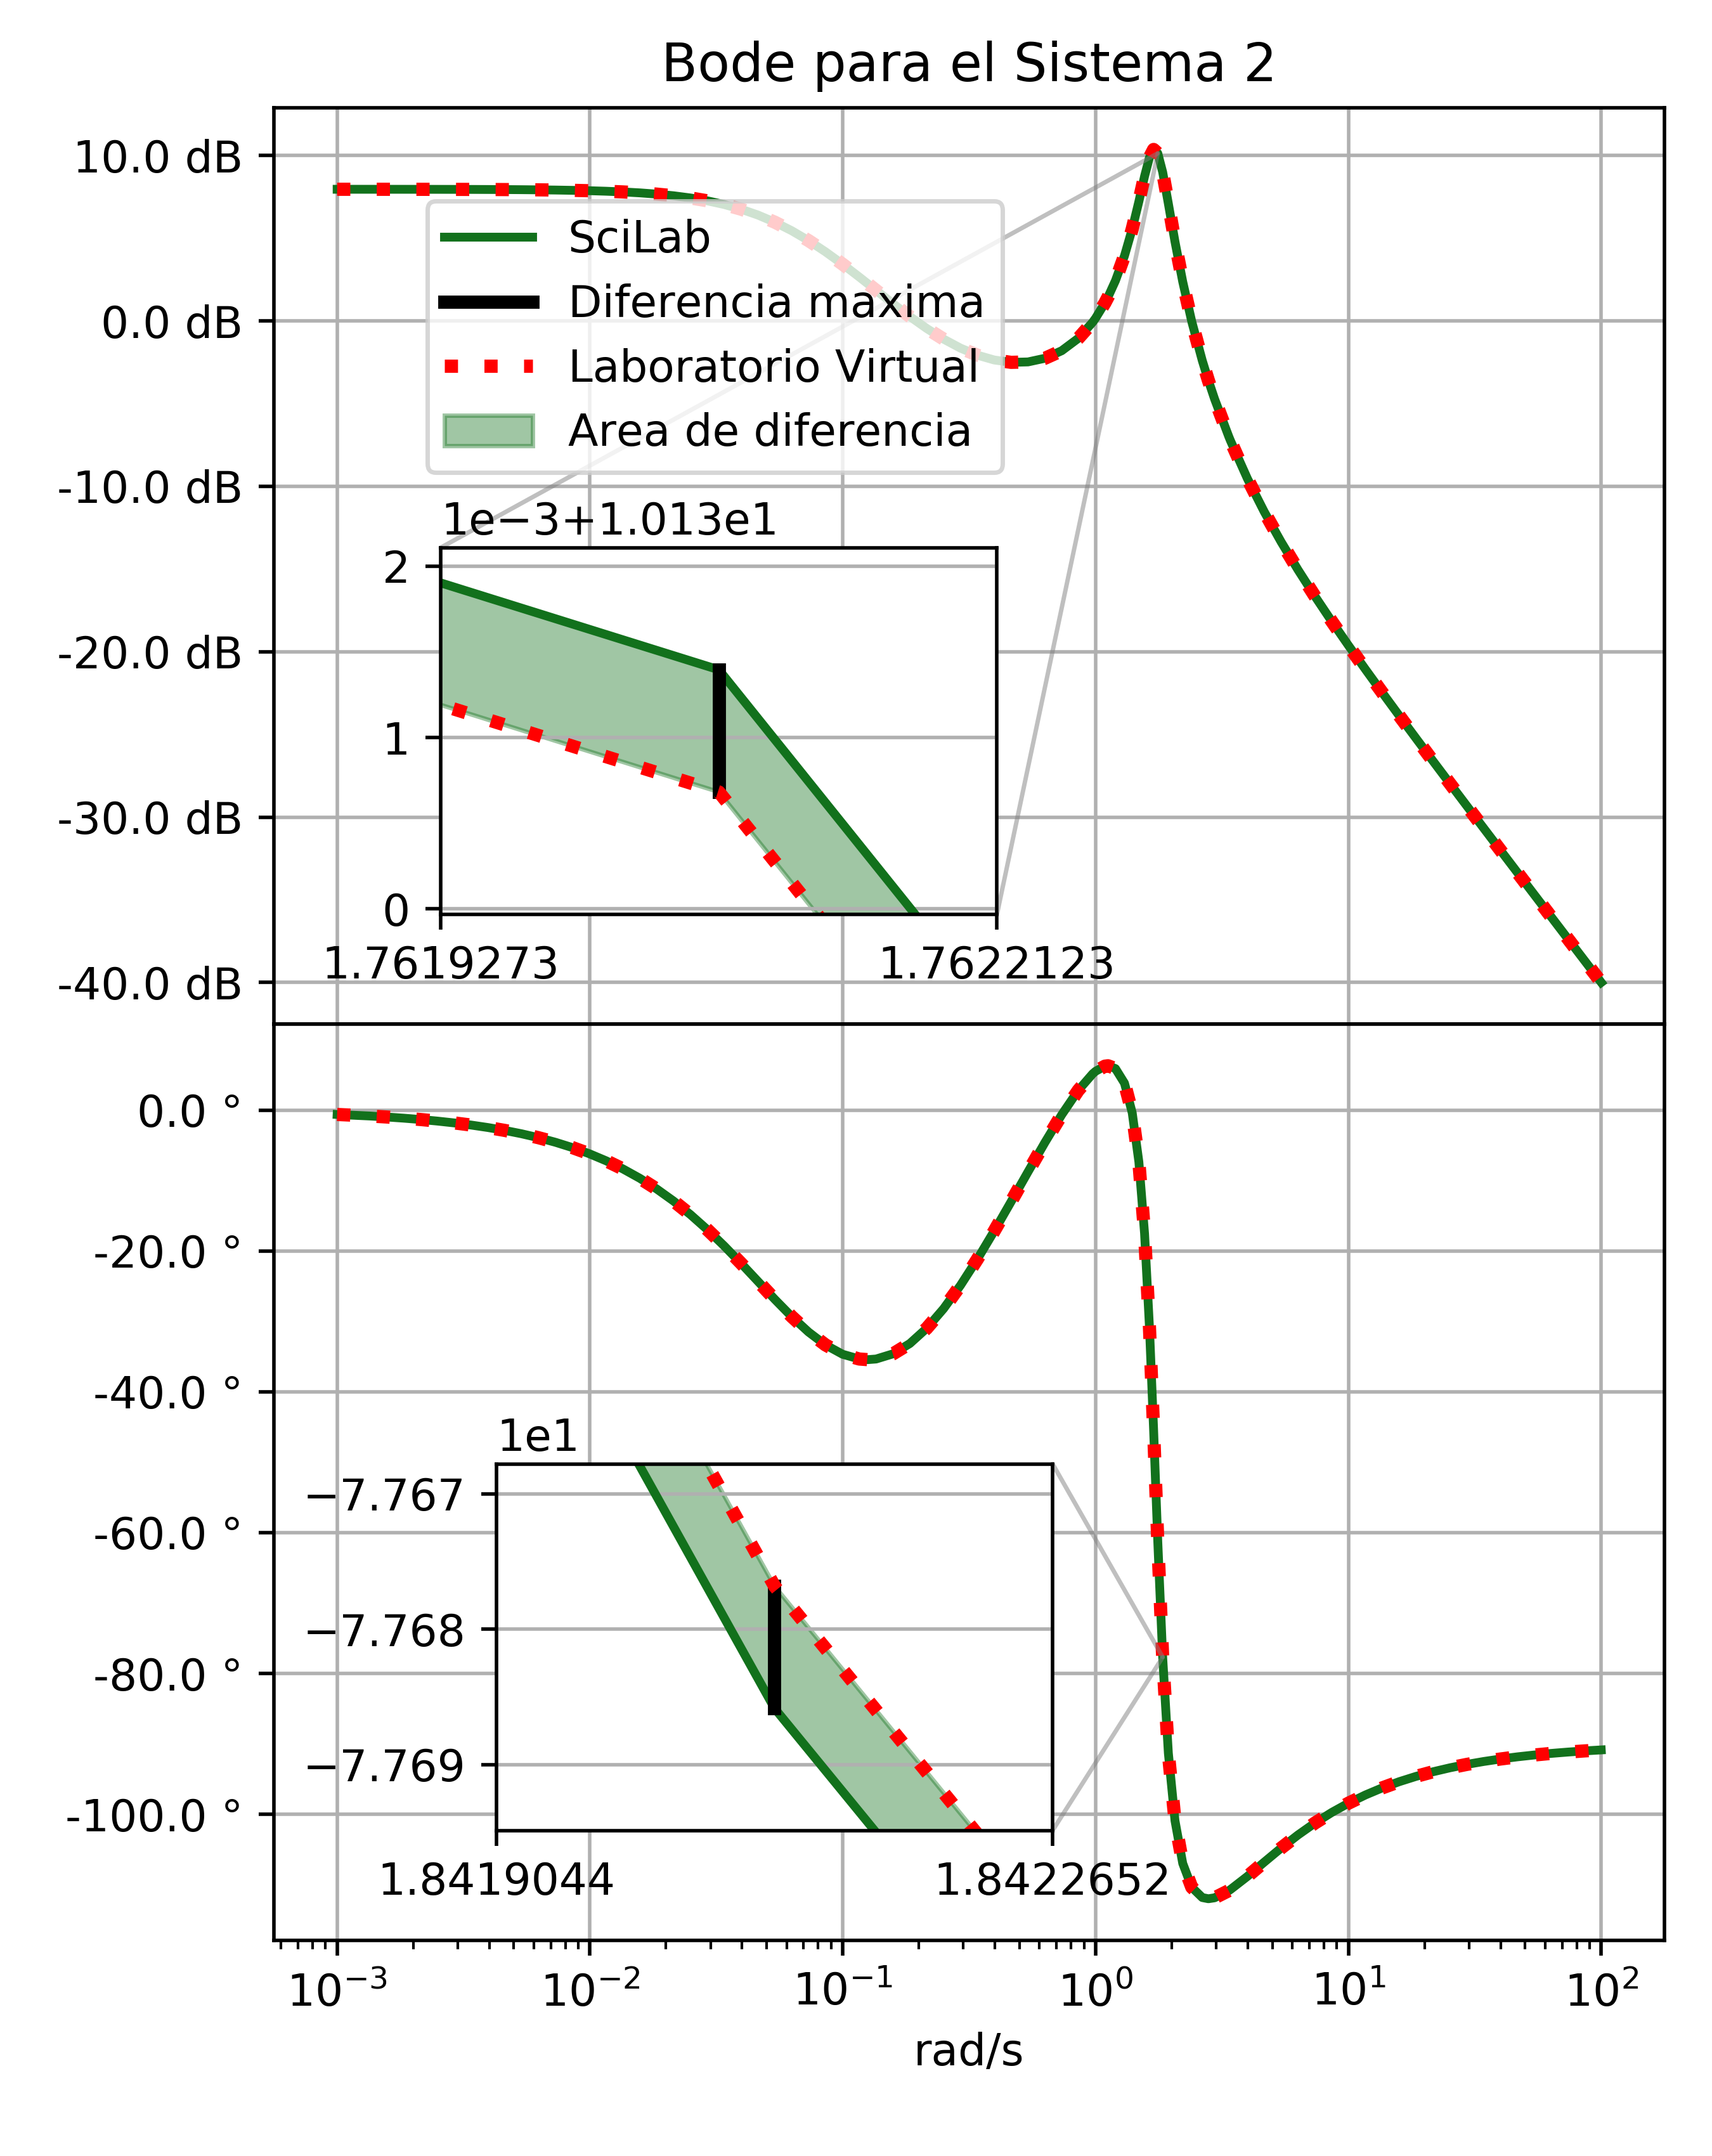
\includegraphics[width=0.49\textwidth,valign=c]{SciLab/ScSet2Bode.png}
            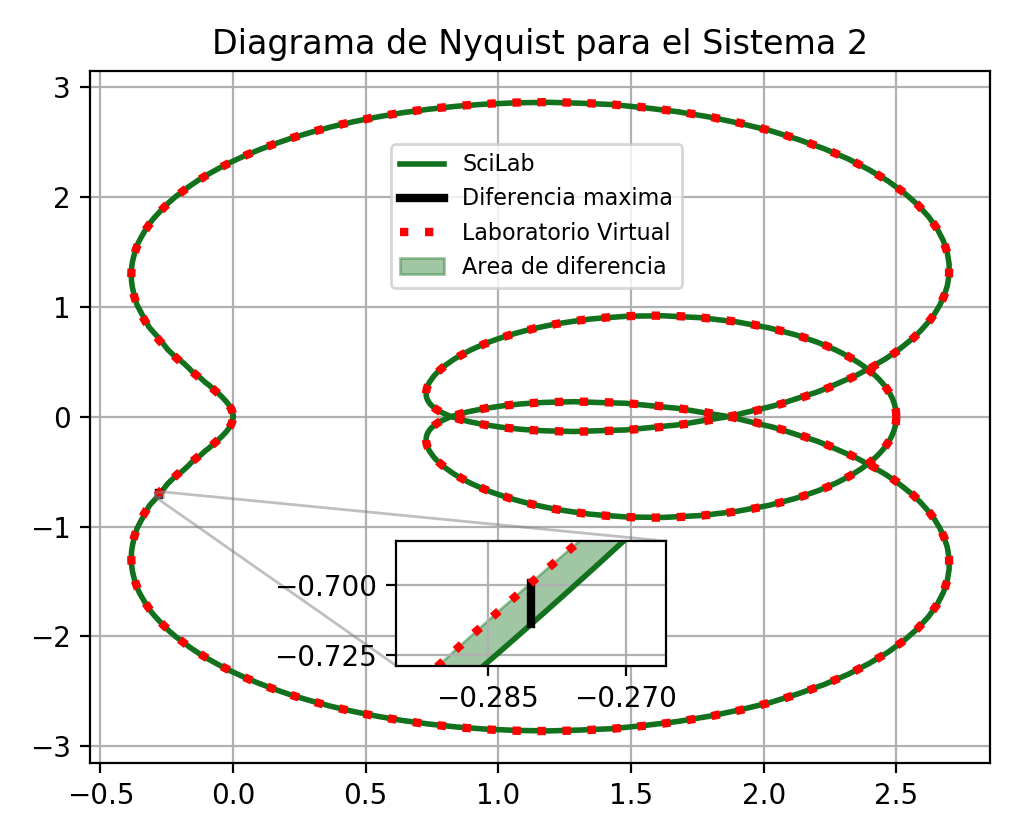
\includegraphics[width=0.49\textwidth,valign=c]{SciLab/ScSet2Nyquist.png}
            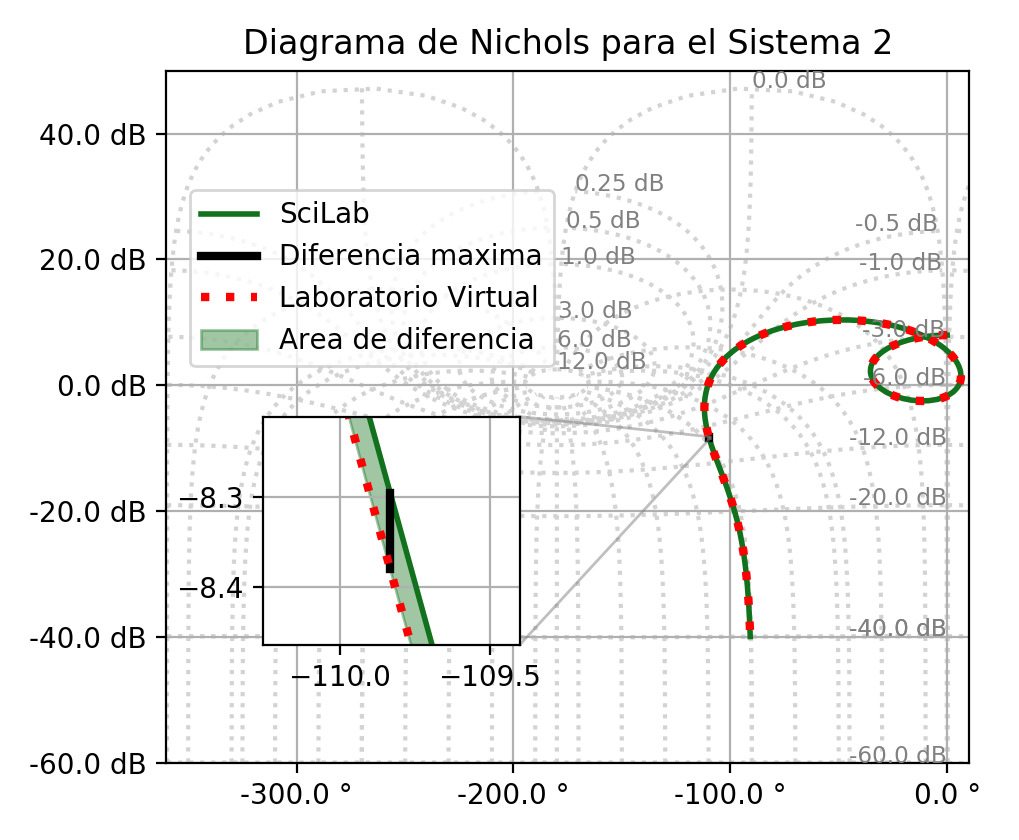
\includegraphics[width=0.49\textwidth,valign=c]{SciLab/ScSet2Nichols.png}
            \label{fig:ScSet2sub}
        \end{subfigure}
        \caption[Comparación de análisis/SciLab - sistema continuo 2]{\textbf{Comparación de análisis/SciLab - sistema continuo 2}. Fuente: Elaboración propia. \label{fig:ScSet2}}
    \end{figure}

    \begin{figure}[htb]
        \centering
        \begin{subfigure}[t]{0.99\textwidth}
            \centering
            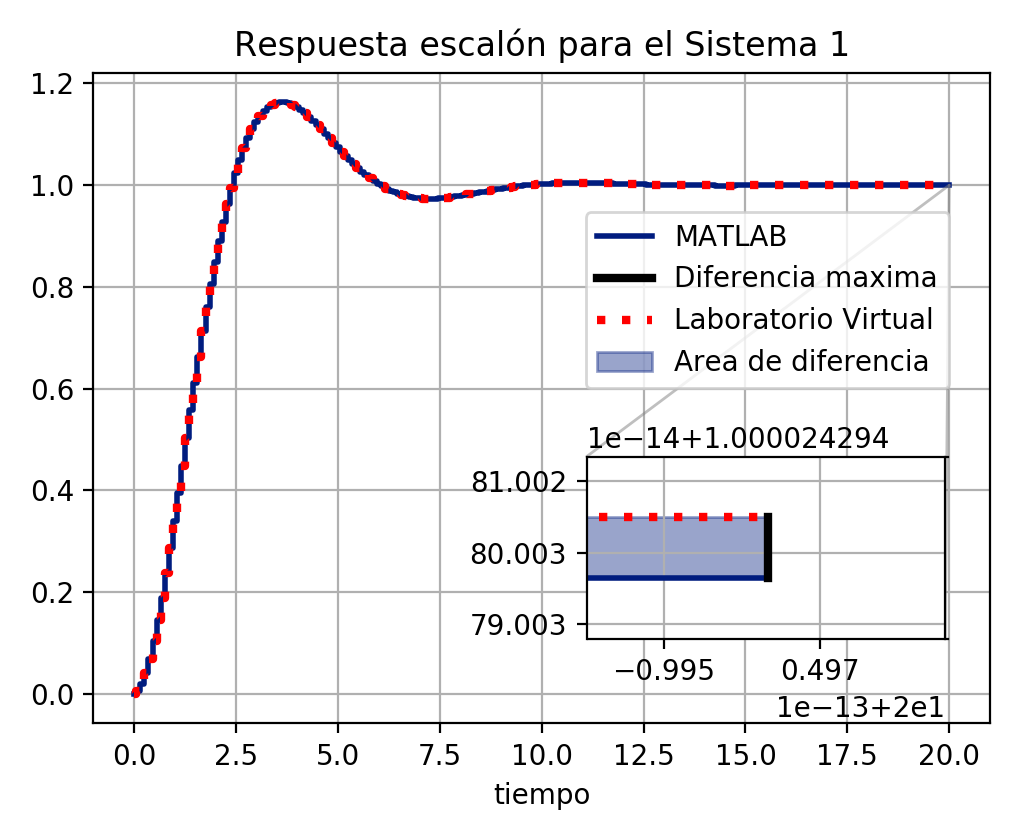
\includegraphics[width=0.49\textwidth,valign=c]{MATLAB/Set1DStep.png}
            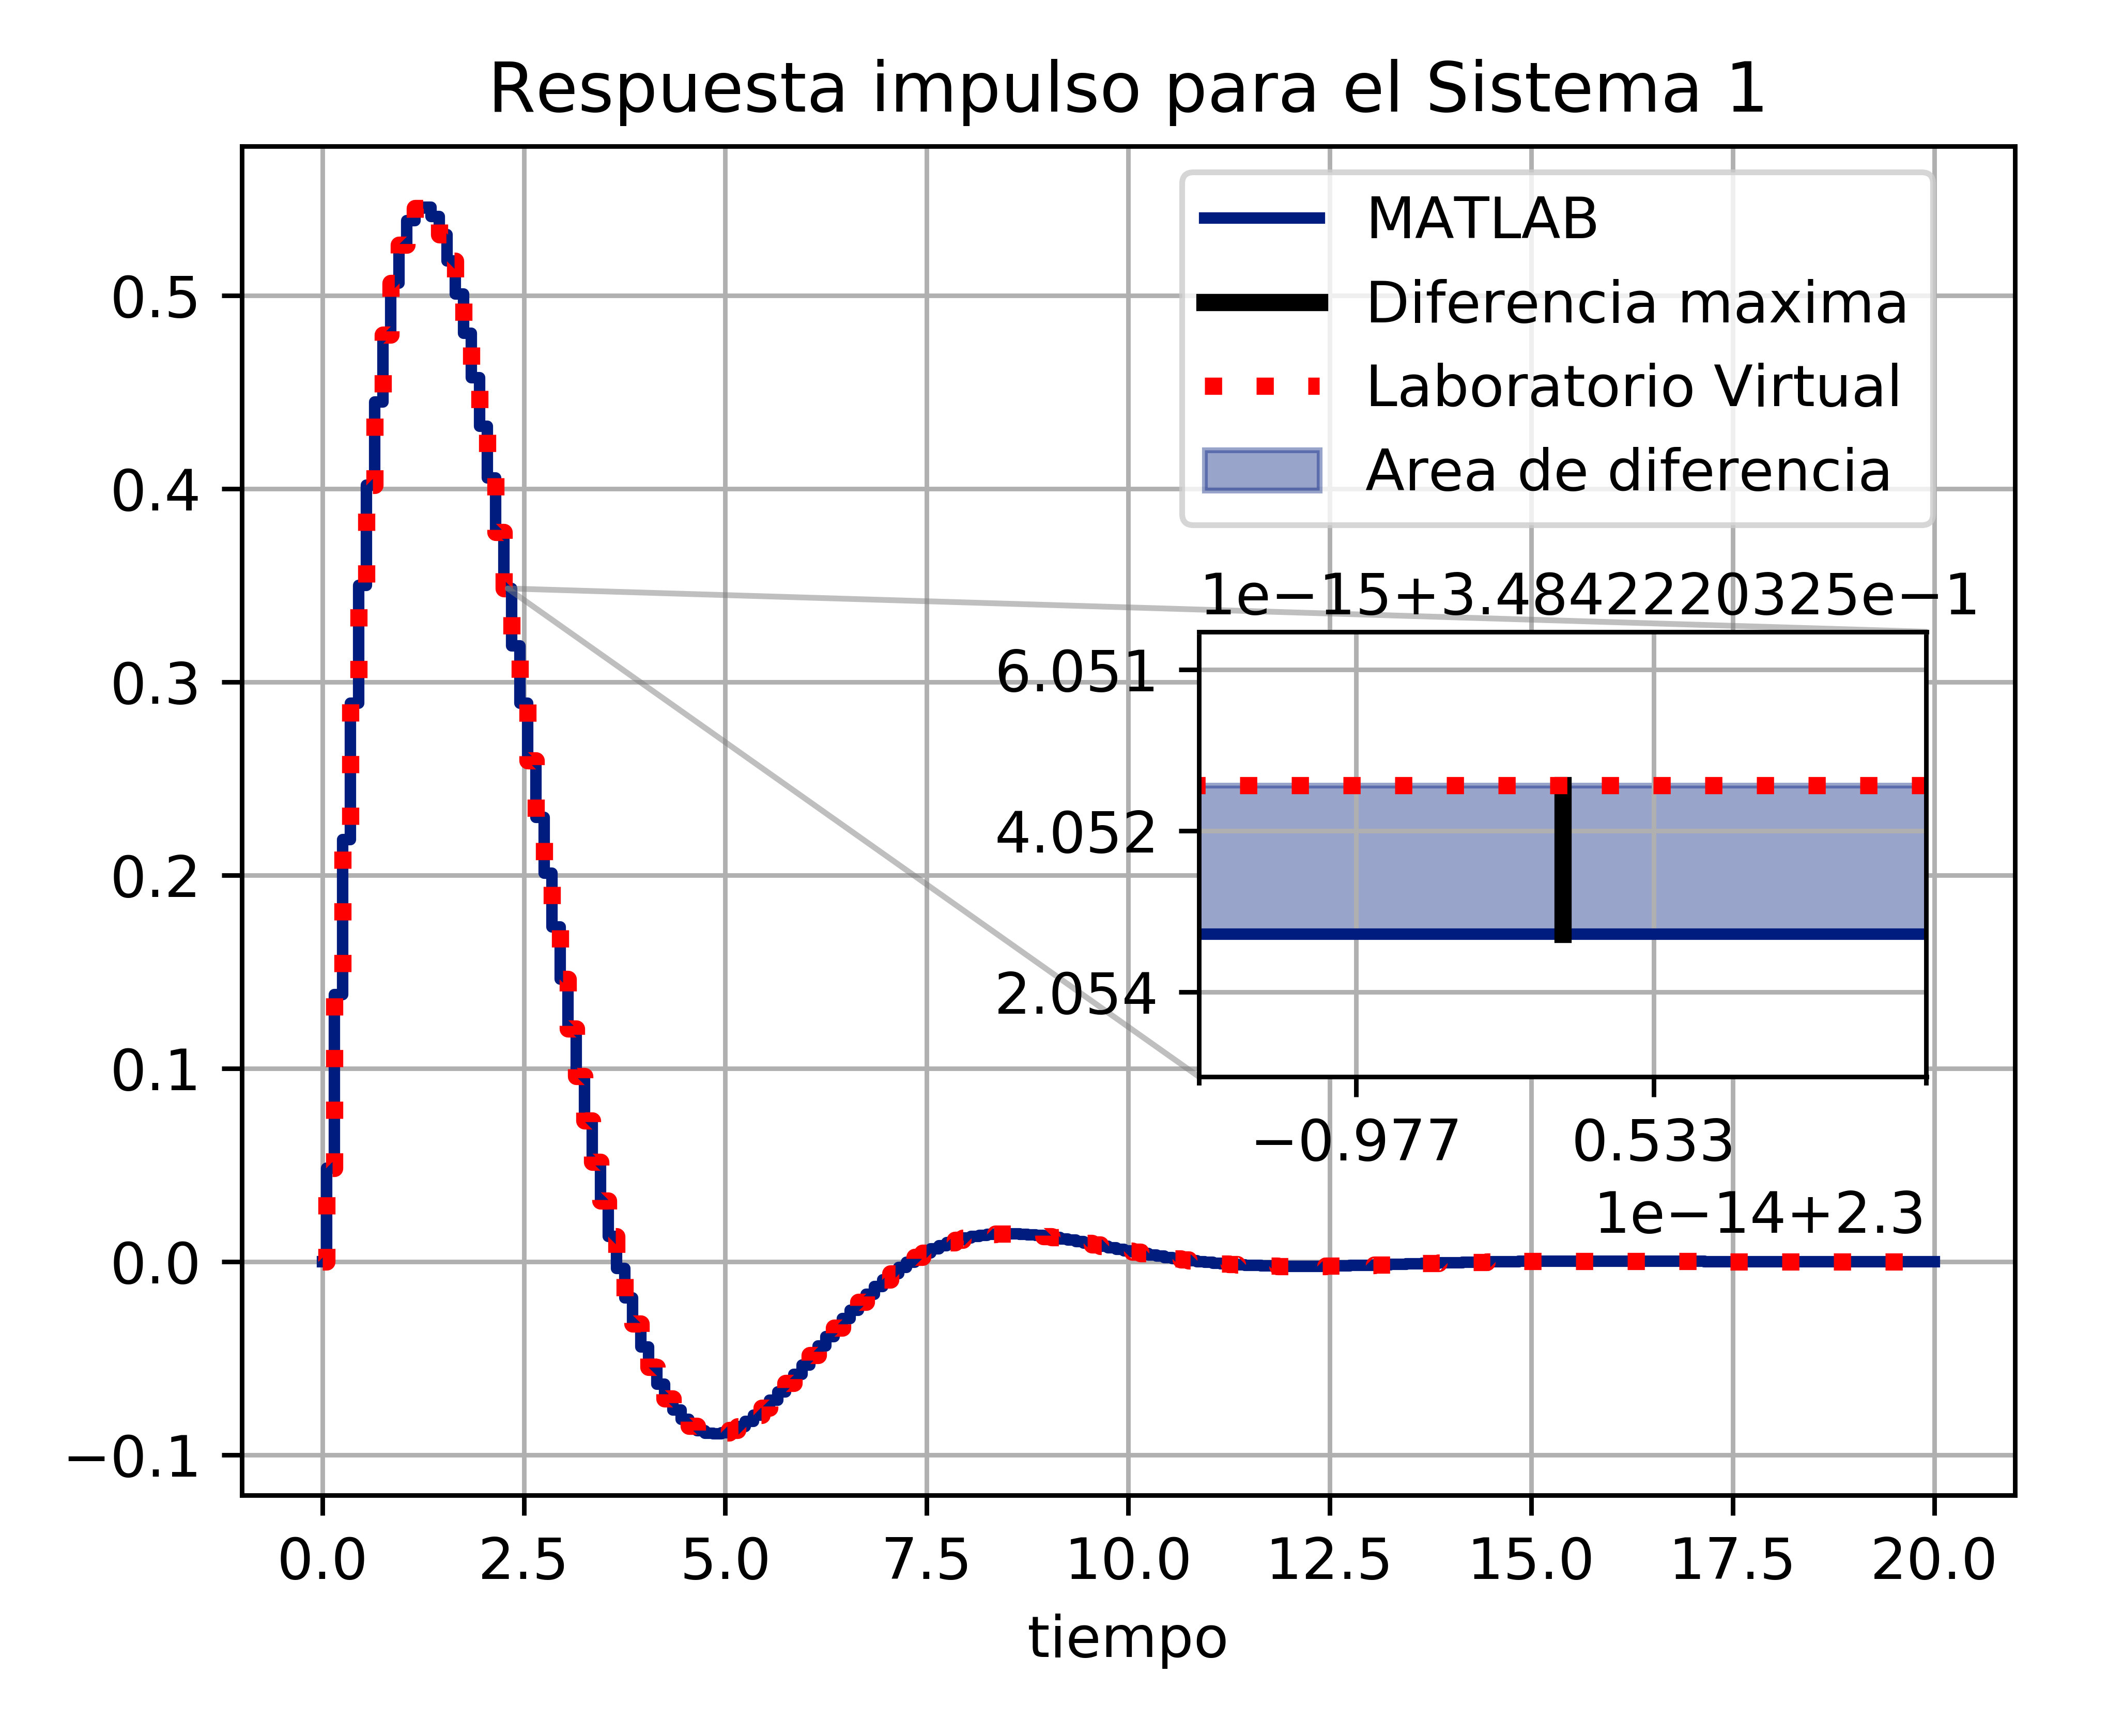
\includegraphics[width=0.49\textwidth,valign=c]{MATLAB/Set1DImp.png}
            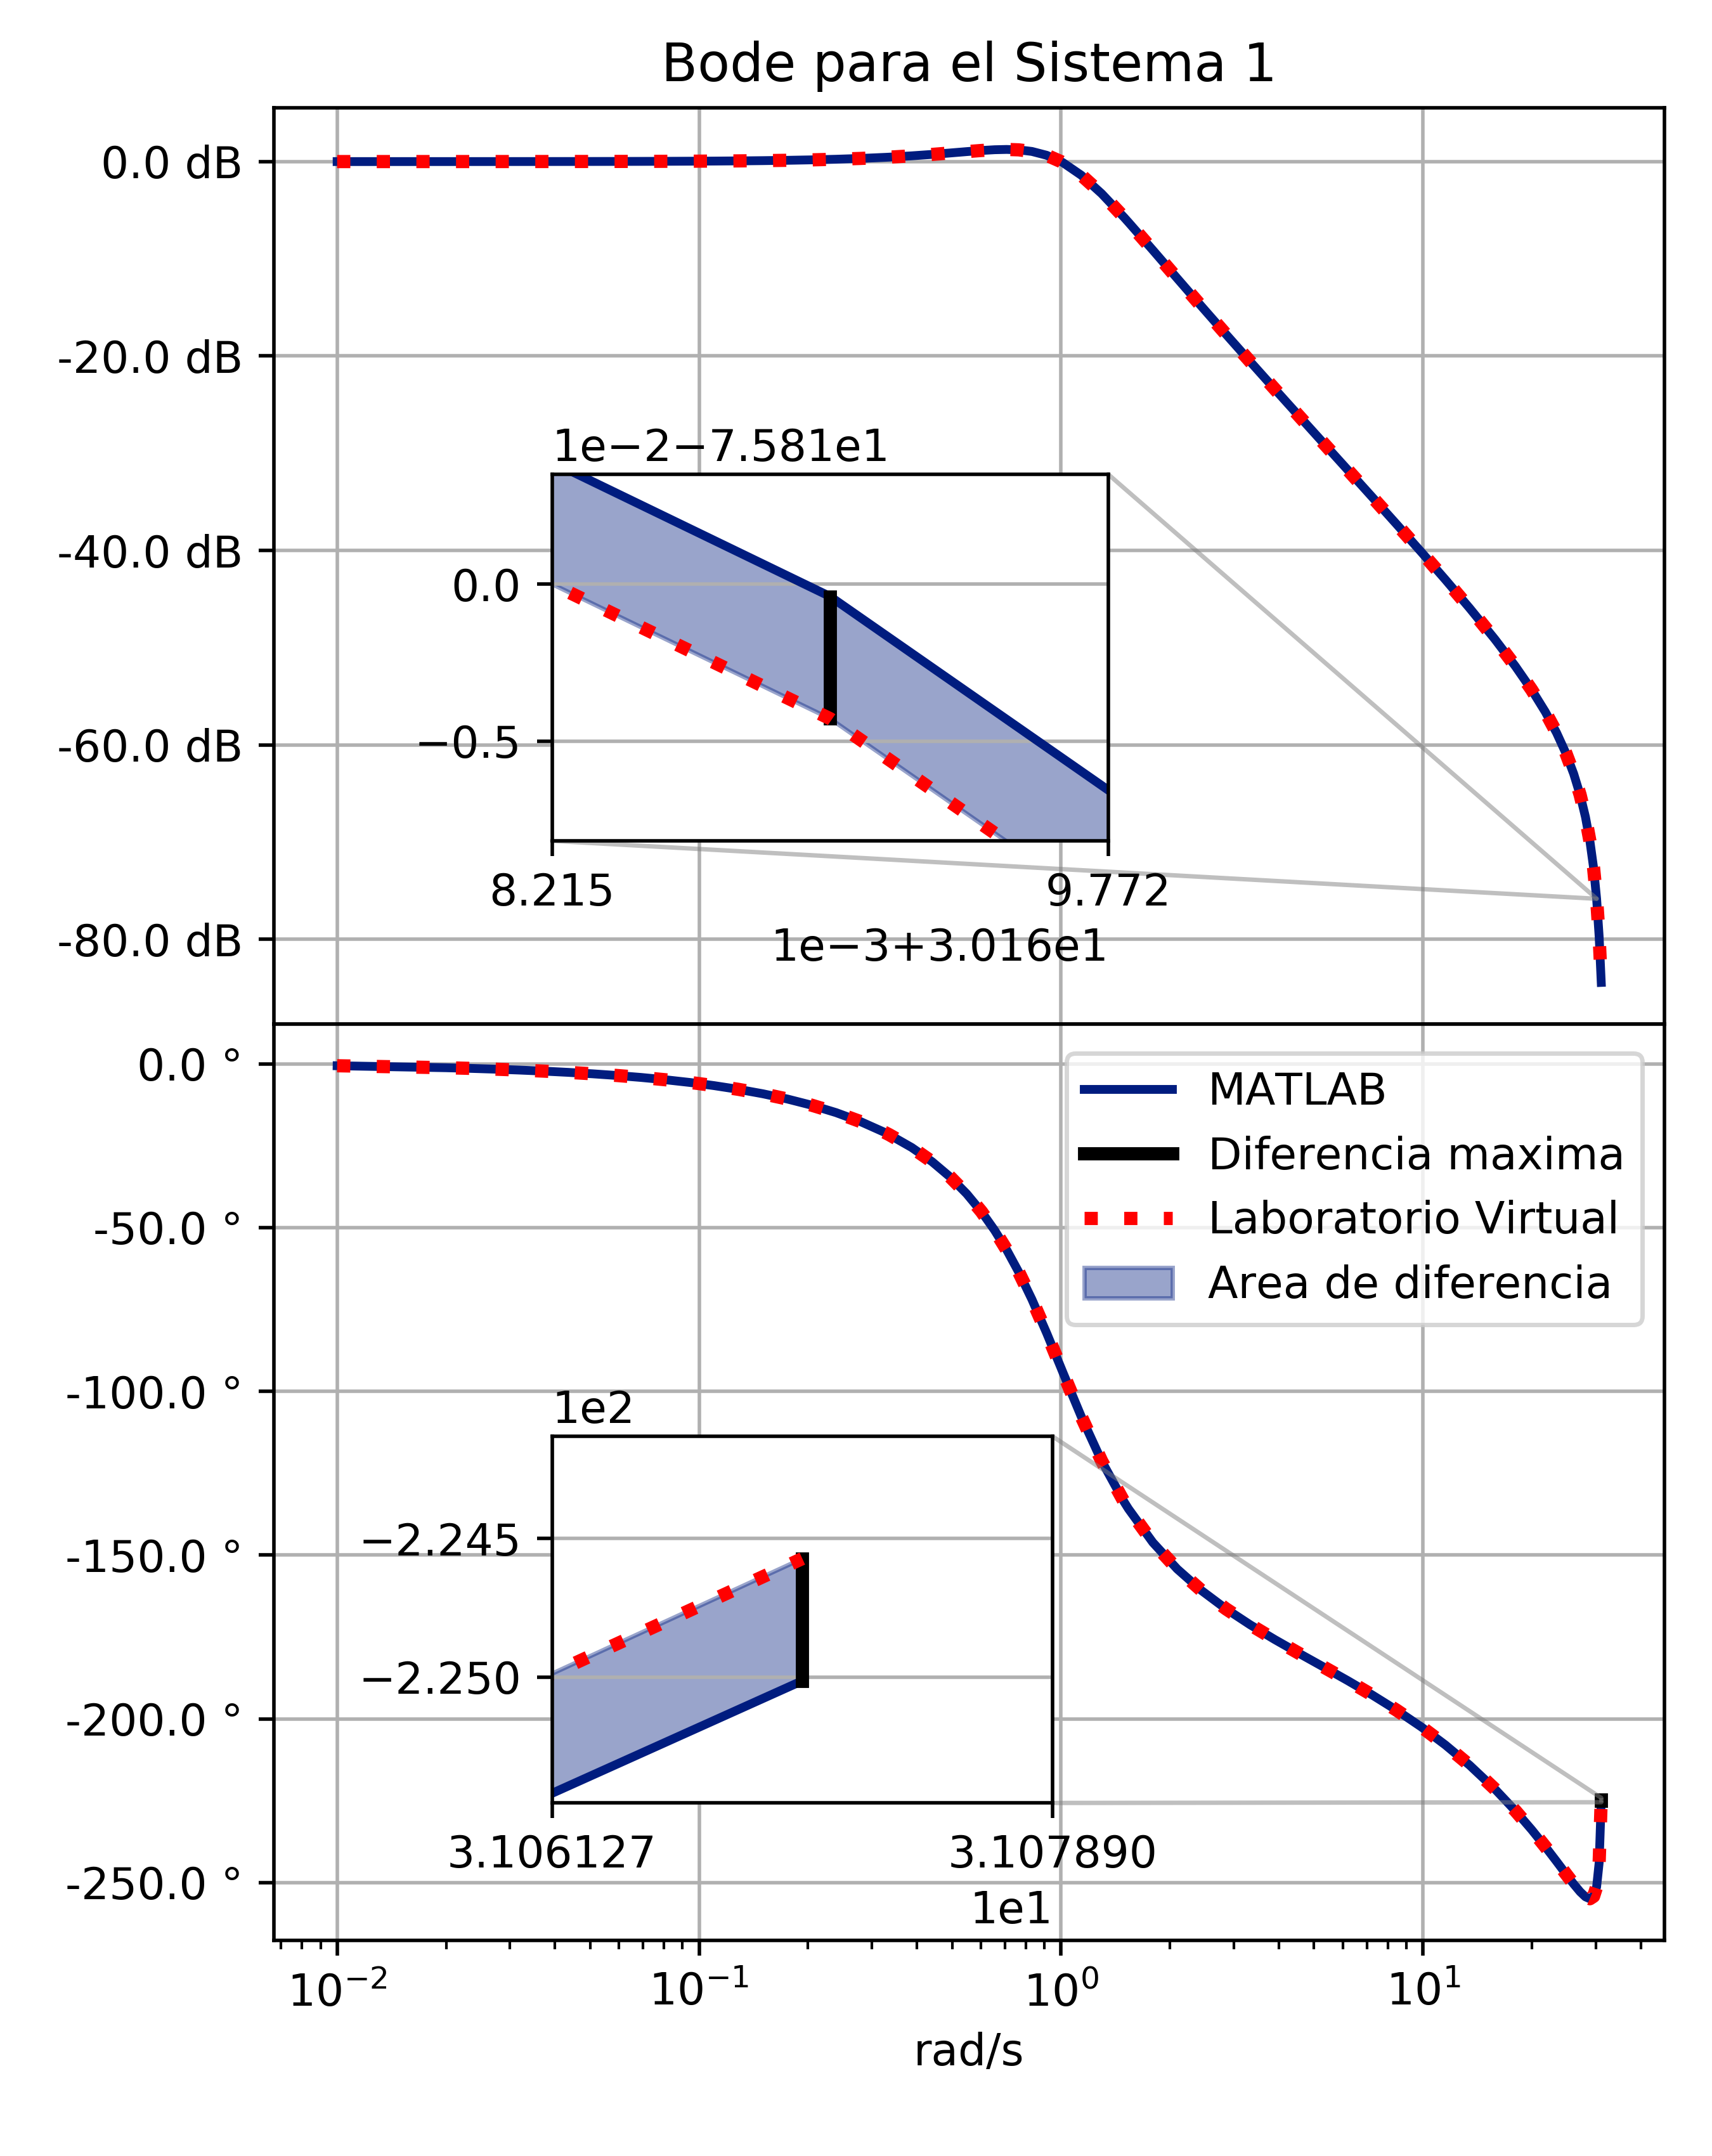
\includegraphics[width=0.49\textwidth,valign=c]{MATLAB/Set1DBode.png}
            \includegraphics[width=0.49\textwidth,valign=c]{MATLAB/Set1DNyquist.png}
            \includegraphics[width=0.49\textwidth,valign=c]{MATLAB/Set1DRlocus.png}
            \includegraphics[width=0.49\textwidth,valign=c]{MATLAB/Set1DNichols.png}
            \label{fig:Set1Dsub}
        \end{subfigure}
        \caption[Comparación de análisis/MATLAB - sistema discreto 1]{\textbf{Comparación de análisis/MATLAB - sistema discreto 1}. Fuente: Elaboración propia. \label{fig:Set1D}}
    \end{figure}

    \begin{figure}[htb]
        \centering
        \begin{subfigure}[t]{0.99\textwidth}
            \centering
            \includegraphics[width=0.49\textwidth,valign=c]{MATLAB/Set2DStep.png}
            \includegraphics[width=0.49\textwidth,valign=c]{MATLAB/Set2DImp.png}
            \includegraphics[width=0.49\textwidth,valign=c]{MATLAB/Set2DBode.png}
            \includegraphics[width=0.49\textwidth,valign=c]{MATLAB/Set2DNyquist.png}
            \includegraphics[width=0.49\textwidth,valign=c]{MATLAB/Set2DRlocus.png}
            \includegraphics[width=0.49\textwidth,valign=c]{MATLAB/Set2DNichols.png}
            \label{fig:Set2Dsub}
        \end{subfigure}
        \caption[Comparación de análisis/MATLAB - sistema discreto 2]{\textbf{Comparación de análisis/MATLAB - sistema discreto 2}. Fuente: Elaboración propia. \label{fig:Set2D}}
    \end{figure}

    \begin{figure}[htb]
        \centering
        \begin{subfigure}[t]{0.99\textwidth}
            \centering
            \includegraphics[width=0.49\textwidth,valign=c]{MATLAB/Set3DStep.png}
            \includegraphics[width=0.49\textwidth,valign=c]{MATLAB/Set3DImp.png}
            \includegraphics[width=0.49\textwidth,valign=c]{MATLAB/Set3DBode.png}
            \includegraphics[width=0.49\textwidth,valign=c]{MATLAB/Set3DNyquist.png}
            \includegraphics[width=0.49\textwidth,valign=c]{MATLAB/Set3DRlocus.png}
            \includegraphics[width=0.49\textwidth,valign=c]{MATLAB/Set3DNichols.png}
            \label{fig:Set3Dsub}
        \end{subfigure}
        \caption[Comparación de análisis/MATLAB - sistema discreto 3]{\textbf{Comparación de análisis/MATLAB - sistema discreto 3}. Fuente: Elaboración propia. \label{fig:Set3D}}
    \end{figure}

    \begin{figure}[htb]
        \centering
        \begin{subfigure}[t]{0.99\textwidth}
            \centering
            \includegraphics[width=0.49\textwidth,valign=c]{SciLab/ScSet1DStep.png}
            \includegraphics[width=0.49\textwidth,valign=c]{SciLab/ScSet1DImp.png}
            \includegraphics[width=0.49\textwidth,valign=c]{SciLab/ScSet1DBode.png}
            \includegraphics[width=0.49\textwidth,valign=c]{SciLab/ScSet1DNyquist.png}
            \includegraphics[width=0.49\textwidth,valign=c]{SciLab/ScSet1DNichols.png}
            \label{fig:ScSet1Dsub}
        \end{subfigure}
        \caption[Comparación de análisis/SciLab - sistema discreto 1]{\textbf{Comparación de análisis/SciLab - sistema discreto 1}. Fuente: Elaboración propia. \label{fig:ScSet1D}}
    \end{figure}

\AgregarAnexo{Estructura FIS para la comparación de diseño de controladores difusos}{anexo:ComparacionDifuso}
    
    Controlador 1:

    \begin{longlisting}				
        \begin{minted}[escapeinside=||,
            mathescape=true,
            autogobble=true,
            fontsize=\scriptsize,
            obeytabs=true,
            tabsize=4,
            baselinestretch=1,
            breaklines]{text}
            [System]
            Name='TomoC1'
            Type='mamdani'
            Version=2.0
            NumInputs=1
            NumOutputs=1
            NumRules=5
            AndMethod='min'
            OrMethod='max'
            ImpMethod='min'
            AggMethod='max'
            DefuzzMethod='centroid'

            [Input1]
            Name='entrada1'
            Range=[-10 10]
            NumMFs=5
            MF1='etiqueta1':'trimf',[-20.0 -10.0 0.0]
            MF2='etiqueta2':'trapmf',[-10.0 -7.5 -2.5 0.0]
            MF3='etiqueta3':'gaussmf',[2.5 0]
            MF4='etiqueta4':'dsigmf',[3 2.5 3 7.5]
            MF5='etiqueta5':'smf',[2.5 10]

            [Output1]
            Name='salida1'
            Range=[-10 10]
            NumMFs=3
            MF1='etiqueta1':'trimf',[-20.0 -10.0 0.0]
            MF2='etiqueta2':'trimf',[-10.0 0.0 10.0]
            MF3='etiqueta3':'trimf',[0.0 10.0 20.0]

            [Rules]
            1, 1 (1.0) : 1
            2, 2 (1.0) : 2
            -3, 3 (1.0) : 2
            4, 2 (1.0) : 1
            5, 1 (0.7999999999999998) : 1
        \end{minted}
    \end{longlisting}

    Controlador 2:

    \begin{longlisting}				
        \begin{minted}[escapeinside=||,
            mathescape=true,
            autogobble=true,
            fontsize=\scriptsize,
            obeytabs=true,
            tabsize=4,
            baselinestretch=1,
            breaklines]{text}
            [System]
            Name='TomoC2'
            Type='mamdani'
            Version=2.0
            NumInputs=2
            NumOutputs=2
            NumRules=9
            AndMethod='min'
            OrMethod='max'
            ImpMethod='min'
            AggMethod='max'
            DefuzzMethod='som'

            [Input1]
            Name='entrada1'
            Range=[-1 1]
            NumMFs=3
            MF1='etiqueta1':'trimf',[-2.0 -1.0 0.0]
            MF2='etiqueta2':'trimf',[-1.0 -0.0 1.0]
            MF3='etiqueta3':'trimf',[0.0 1.0 2.0]

            [Input2]
            Name='entrada2'
            Range=[-10 10]
            NumMFs=3
            MF1='etiqueta1':'trimf',[-20.0 -10.0 0.0]
            MF2='etiqueta2':'trimf',[-10.0 0.0 10.0]
            MF3='etiqueta3':'trimf',[0.0 10.0 20.0]

            [Output1]
            Name='salida1'
            Range=[-1 1]
            NumMFs=3
            MF1='etiqueta1':'trimf',[-2.0 -1.0 0.0]
            MF2='etiqueta2':'trimf',[-1.0 -0.0 1.0]
            MF3='etiqueta3':'trimf',[0.0 1.0 2.0]

            [Output2]
            Name='salida2'
            Range=[-100 100]
            NumMFs=3
            MF1='etiqueta1':'trimf',[-200.0 -100.0 0.0]
            MF2='etiqueta2':'trimf',[-100.0 0.0 100.0]
            MF3='etiqueta3':'trimf',[0.0 100.0 200.0]

            [Rules]
            1 1, 1 1 (1.0) : 1
            1 2, 2 1 (1.0) : 2
            1 -3, 3 1 (1.0) : 2
            -2 2, 3 2 (1.0) : 2
            -2 1, 3 3 (1.0) : 1
            2 -3, 3 1 (1.0) : 1
            3 1, 1 3 (0.8999999999999999) : 1
            3 2, 2 2 (0.7499999999999998) : 1
            -3 -3, 3 1 (0.7499999999999998) : 1
        \end{minted}
    \end{longlisting}

\AgregarAnexo{Estructura FIS para la comparación de simulación de sistemas de control}{anexo:ComparacionFISim}
    
    Controlador PID difuso:

    \begin{longlisting}				
        \begin{minted}[escapeinside=||,
            mathescape=true,
            autogobble=true,
            fontsize=\scriptsize,
            obeytabs=true,
            tabsize=4,
            baselinestretch=1,
            breaklines]{text}
            [System]
            Name='PIDdifuso'
            Type='mamdani'
            Version=2.0
            NumInputs=3
            NumOutputs=1
            NumRules=29
            AndMethod='min'
            OrMethod='max'
            ImpMethod='min'
            AggMethod='max'
            DefuzzMethod='centroid'

            [Input1]
            Name='error'
            Range=[-1 1]
            NumMFs=3
            MF1='negativo':'trimf',[-2.0 -1.0 0.0]
            MF2='cero':'trimf',[-1.0 0.0 1.0]
            MF3='positivo':'trimf',[0.0 1.0 2.0]

            [Input2]
            Name='d_error'
            Range=[-1 1]
            NumMFs=3
            MF1='negativo':'trimf',[-2.0 -1.0 0.0]
            MF2='cero':'trimf',[-1.0 0.0 1.0]
            MF3='positivo':'trimf',[0.0 1.0 2.0]

            [Input3]
            Name='d2_error'
            Range=[-1 1]
            NumMFs=3
            MF1='negativo':'trimf',[-2.0 -1.0 0.0]
            MF2='cero':'trimf',[-1.0 0.0 1.0]
            MF3='positivo':'trimf',[0.0 1.0 2.0]

            [Output1]
            Name='scontrol'
            Range=[-2 2]
            NumMFs=3
            MF1='negativa':'trimf',[-3.0 -2.0 0]
            MF2='cero':'trimf',[-2.0 0 2.0]
            MF3='positiva':'trimf',[0 2.0 3.0]

            [Rules]
            2 2 3, 2 (1.0) : 1
            2 2 2, 2 (1.0) : 1
            2 2 1, 2 (1.0) : 1
            2 3 1, 3 (1.0) : 1
            2 3 2, 2 (1.0) : 1
            2 3 3, 2 (1.0) : 1
            2 1 3, 1 (1.0) : 1
            2 1 2, 2 (1.0) : 1
            2 1 1, 2 (1.0) : 1
            3 1 1, 3 (1.0) : 1
            3 1 2, 3 (1.0) : 1
            3 1 3, 1 (1.0) : 1
            3 3 1, 2 (1.0) : 1
            3 3 2, 1 (1.0) : 1
            3 3 3, 2 (1.0) : 1
            3 2 1, 3 (1.0) : 1
            3 2 2, 3 (1.0) : 1
            3 2 3, 3 (1.0) : 1
            1 1 1, 1 (1.0) : 1
            1 1 2, 1 (1.0) : 1
            1 1 3, 2 (1.0) : 1
            1 3 1, 3 (1.0) : 1
            1 3 2, 3 (1.0) : 1
            1 3 3, 2 (1.0) : 1
            1 2 1, 1 (1.0) : 1
            1 2 2, 1 (1.0) : 1
            1 2 3, 1 (1.0) : 1
            -2 1 0, 3 (1.0) : 1
            -2 3 0, 1 (1.0) : 1
        \end{minted}
    \end{longlisting}

    Controlador PI difuso:

    \begin{longlisting}				
        \begin{minted}[escapeinside=||,
            mathescape=true,
            autogobble=true,
            fontsize=\scriptsize,
            obeytabs=true,
            tabsize=4,
            baselinestretch=1,
            breaklines]{text}
            [System]
            Name='PI'
            Type='mamdani'
            Version=2.0
            NumInputs=2
            NumOutputs=1
            NumRules=9
            AndMethod='min'
            OrMethod='max'
            ImpMethod='min'
            AggMethod='max'
            DefuzzMethod='centroid'

            [Input1]
            Name='error'
            Range=[-1 1]
            NumMFs=3
            MF1='negativo':'sigmf',[-12.0 -0.5]
            MF2='cero':'dsigmf',[12.0 -0.5 12.0 0.5]
            MF3='positivo':'sigmf',[12.0 0.5]

            [Input2]
            Name='d_error'
            Range=[-2 2]
            NumMFs=3
            MF1='negativo':'sigmf',[-6.0 -1]
            MF2='cero':'dsigmf',[6.0 -1 6.0 1]
            MF3='positivo':'sigmf',[6.0 1]

            [Output1]
            Name='s_control'
            Range=[-1 1]
            NumMFs=3
            MF1='negativa':'zmf',[-1 0]
            MF2='cero':'pimf',[-1 0 0 1]
            MF3='positiva':'smf',[0 1]

            [Rules]
            3 1, 3 (1.0) : 1
            1 3, 1 (1.0) : 1
            3 2, 3 (0.49999999999999956) : 1
            1 2, 1 (0.5) : 1
            2 1, 2 (0.2) : 1
            2 2, 2 (0.2) : 1
            2 3, 2 (0.2) : 1
            3 3, 1 (1.0) : 1
            1 1, 3 (1.0) : 1
        \end{minted}
    \end{longlisting}

    Controlador PD difuso:

    \begin{longlisting}				
        \begin{minted}[escapeinside=||,
            mathescape=true,
            autogobble=true,
            fontsize=\scriptsize,
            obeytabs=true,
            tabsize=4,
            baselinestretch=1,
            breaklines]{text}
            [System]
            Name='PD'
            Type='mamdani'
            Version=2.0
            NumInputs=2
            NumOutputs=1
            NumRules=9
            AndMethod='min'
            OrMethod='max'
            ImpMethod='min'
            AggMethod='max'
            DefuzzMethod='centroid'

            [Input1]
            Name='error'
            Range=[-1 1]
            NumMFs=3
            MF1='negativo':'gaussmf',[0.5 -1.0]
            MF2='cero':'gaussmf',[0.3 0.0]
            MF3='positivo':'gaussmf',[0.5 1.0]

            [Input2]
            Name='d_error'
            Range=[-1 1]
            NumMFs=3
            MF1='negativo':'gaussmf',[0.5 -1.0]
            MF2='cero':'gaussmf',[0.3 0.0]
            MF3='positivo':'gaussmf',[0.5 1.0]

            [Output1]
            Name='s_control'
            Range=[-1 1]
            NumMFs=3
            MF1='negativa':'trapmf',[-2.0 -1.5 -0.85 0.0]
            MF2='cero':'trapmf',[-1.0 -0.1 0.1 1.0]
            MF3='positiva':'trapmf',[0.0 0.85 1.5 2.0]

            [Rules]
            2 1, 2 (0.5) : 1
            2 2, 2 (1.0) : 1
            2 3, 2 (0.5) : 1
            3 3, 3 (1.0) : 1
            3 2, 3 (1.0) : 1
            3 1, 2 (0.25) : 1
            1 1, 1 (1.0) : 1
            1 2, 1 (1.0) : 1
            1 3, 2 (0.25) : 1
        \end{minted}
    \end{longlisting}

    Controlador programador de ganancias (PDG) difuso:

    \begin{longlisting}				
        \begin{minted}[escapeinside=||,
            mathescape=true,
            autogobble=true,
            fontsize=\scriptsize,
            obeytabs=true,
            tabsize=4,
            baselinestretch=1,
            breaklines]{text}
            [System]
            Name='PDG'
            Type='mamdani'
            Version=2.0
            NumInputs=2
            NumOutputs=3
            NumRules=9
            AndMethod='min'
            OrMethod='max'
            ImpMethod='min'
            AggMethod='max'
            DefuzzMethod='centroid'

            [Input1]
            Name='Error'
            Range=[-1 1]
            NumMFs=3
            MF1='negativo':'trimf',[-2.0 -1.0 0.0]
            MF2='cero':'trimf',[-1.0 0.0 1.0]
            MF3='positivo':'trimf',[0.0 1.0 2.0]

            [Input2]
            Name='Derivada del Error'
            Range=[-1 1]
            NumMFs=3
            MF1='negativa':'trimf',[-2.0 -1.0 0.0]
            MF2='cero':'trimf',[-1.0 0.0 1.0]
            MF3='positiva':'trimf',[0.0 1.0 2.0]

            [Output1]
            Name='Kp'
            Range=[0 2]
            NumMFs=3
            MF1='Cero':'trimf',[-1 0 1]
            MF2='alto':'trimf',[0 1 2]
            MF3='muy alto':'trimf',[1 2 3]

            [Output2]
            Name='Ki'
            Range=[0 2]
            NumMFs=3
            MF1='Cero':'trimf',[-1 0 1]
            MF2='alto':'trimf',[0 1 2]
            MF3='muy alto':'trimf',[1 2 3]

            [Output3]
            Name='Kd'
            Range=[0 1]
            NumMFs=3
            MF1='Cero':'trimf',[-1.0 0 0.5]
            MF2='alto':'trimf',[0 0.5 1]
            MF3='muy alto':'trimf',[0.5 1 2]

            [Rules]
            1 1, 1 1 2 (1.0) : 1
            1 2, 2 2 2 (1.0) : 1
            1 3, 3 3 2 (1.0) : 1
            2 1, 1 1 1 (1.0) : 1
            2 2, 2 2 1 (1.0) : 1
            2 3, 2 2 1 (1.0) : 1
            3 1, 3 3 3 (1.0) : 1
            3 2, 3 3 2 (1.0) : 1
            3 3, 1 1 2 (1.0) : 1
        \end{minted}
    \end{longlisting}

    Controlador difuso simple:

    \begin{longlisting}				
        \begin{minted}[escapeinside=||,
            mathescape=true,
            autogobble=true,
            fontsize=\scriptsize,
            obeytabs=true,
            tabsize=4,
            baselinestretch=1,
            breaklines]{text}
            [System]
            Name='simpleF'
            Type='mamdani'
            Version=2.0
            NumInputs=1
            NumOutputs=1
            NumRules=5
            AndMethod='min'
            OrMethod='max'
            ImpMethod='min'
            AggMethod='max'
            DefuzzMethod='centroid'

            [Input1]
            Name='error'
            Range=[-1 1]
            NumMFs=5
            MF1='negativo grande':'trimf',[-2 -1 -0.5]
            MF2='negativo':'trimf',[-1 -0.5 0]
            MF3='cero':'trimf',[-0.5 0 0.5]
            MF4='positivo':'trimf',[0 0.5 1.0]
            MF5='positivo grande':'trimf',[0.5 1.0 2]

            [Output1]
            Name='s_fuzzy'
            Range=[-1 1]
            NumMFs=5
            MF1='negativa grande':'trimf',[-2 -1 -0.5]
            MF2='negativa':'trimf',[-1 -0.5 0]
            MF3='cero':'trimf',[-0.5 0.0 0.5]
            MF4='positiva':'trimf',[0 0.5 1.0]
            MF5='positiva grande':'trimf',[0.5 1.0 1.667]

            [Rules]
            5, 5 (1.0) : 1
            4, 4 (0.49999999999999956) : 1
            3, 3 (0.09999999999999924) : 1
            2, 2 (0.49999999999999956) : 1
            1, 1 (1.0) : 1
        \end{minted}
    \end{longlisting}

\AgregarAnexo{Comparación de simulación de sistemas de control}{anexo:ComparacionSimC}
    
    \addtocontents{lof}{\protect\hfill\par\bigskip}
    \addtocontents{lof}{\protect\hspace{-1.5cm}FIGURA~\hfill Pág.\par}
    \addtocontents{lof}{\protect~\hfill\par}

    \begin{figure}[!h]
        \centering
        \begin{subfigure}[t]{0.99\textwidth}
            \centering
            \includegraphics[width=0.49\textwidth,valign=c]{LV/Pc.pdf}
            \includegraphics[width=0.49\textwidth,valign=c]{LV/PIc.pdf}
            \includegraphics[width=0.49\textwidth,valign=c]{LV/PIDc.pdf}
            \includegraphics[width=0.49\textwidth,valign=c]{LV/PImasDc.pdf}
            \includegraphics[width=0.49\textwidth,valign=c]{LV/PDmasIc.pdf}
            \includegraphics[width=0.49\textwidth,valign=c]{LV/PDGc1.pdf}
            \label{fig:simC1}
        \end{subfigure}
        \caption[Comparación de simulación de sistemas de control continuos - 1]{\textbf{Comparación de simulación de sistemas de control en tiempo continuo - 1}. Controladores: P, PI, PID, PI difuso + D, PD difuso + I y PDG. Fuente: Elaboración propia. \label{fig:simC1f}}
    \end{figure}

    \begin{figure}[htb]
        \centering
        \begin{subfigure}[t]{0.99\textwidth}
            \centering
            \includegraphics[width=0.49\textwidth,valign=c]{LV/PDGc2.pdf}
            \includegraphics[width=0.49\textwidth,valign=c]{LV/PIDmasfc.pdf}
            \label{fig:simC2}
        \end{subfigure}
        \caption[Comparación de simulación de sistemas de control continuos - 2]{\textbf{Comparación de simulación de sistemas de control en tiempo continuo - 2}. Controladores: PDG con saturador y PID + difuso simple. Fuente: Elaboración propia. \label{fig:simC2f}}
    \end{figure}

    \begin{figure}[htb]
        \centering
        \begin{subfigure}[t]{0.99\textwidth}
            \centering
            \includegraphics[width=0.49\textwidth,valign=c]{LV/Pd.pdf}
            \includegraphics[width=0.49\textwidth,valign=c]{LV/PId.pdf}
            \includegraphics[width=0.49\textwidth,valign=c]{LV/PIDd.pdf}
            \includegraphics[width=0.49\textwidth,valign=c]{LV/PIDdf.pdf}
            \label{fig:simD1}
        \end{subfigure}
        \caption[Comparación de simulación de sistemas de control discretos - 1]{\textbf{Comparación de simulación de sistemas de control en tiempo discreto - 1}. Controladores: P, PI, PID y PID difuso. Fuente: Elaboración propia. \label{fig:simD1f}}
    \end{figure}

    \begin{figure}[htb]
        \centering
        \begin{subfigure}[t]{0.99\textwidth}
            \centering
            \includegraphics[width=0.49\textwidth,valign=c]{LV/PImasDd.pdf}
            \includegraphics[width=0.49\textwidth,valign=c]{LV/PDmasId.pdf}
            \includegraphics[width=0.49\textwidth,valign=c]{LV/PIDmasfd.pdf}
            \label{fig:simD2}
        \end{subfigure}
        \caption[Comparación de simulación de sistemas de control discretos - 2]{\textbf{Comparación de simulación de sistemas de control en tiempo discreto - 2}. Controladores: PI difuso + D, PD difuso + I y PID + difuso simple. Fuente: Elaboración propia. \label{fig:simD2f}}
    \end{figure}